%!TEX root = ../../PhD_thesis__Edouard_Leurent.tex

\graphicspath{{2-Chapters/7-Chapter/}}

\chapter{Preparing for the Worst}
\label{chapter:7}

\begin{flushright}
	\begin{tabular}{@{}l@{}}
		\emph{Two roads diverged in a wood, and I--}\\
		\emph{I took the one less traveled by,}\\
		\emph{And that has made all the difference.}\\
	\end{tabular}
	
	Robert Frost, \href{https://eleurent.github.io/sisyphe/texts/the-road-not-taken.html}{\emph{The Road Not Taken}}.
\end{flushright}

\abstractStartChapter{}%
This chapter\dots
\minitocStartChapter{}


Despite the recent successes of Reinforcement Learning in cracking many hard problems \citep[e.g.][]{mnih2015humanlevel,Silver1140}, this tool has hardly been applied in real industrial issues. This could be attributed to two undesirable properties which limit its practical applications. First, it depends on a tremendous amount of interaction data that cannot always be simulated. This issue is alleviated by model-based methods -- which we consider in this work -- that benefit from better sample efficiencies by exploiting a richer data stream than their model-free counterparts. Second, it relies on trial-and-error and random exploration. In this paper, we consider the problem of controlling an unknown linear system $x(t)$ so as to maximise an \emph{arbitrary} bounded reward function $R$, in a critical setting where mistakes are costly and must be avoided at all time. 
This choice of rich reward space is crucial to have sufficient flexibility to model non-convex and non-smooth functions that naturally arise in many practical problems involving combinatorial optimisation, branching decisions, etc., while quadratic costs are mostly suited for tracking a reference trajectory already known a priori \citep[e.g.][]{Kumar2013}.

Since experiencing failures is out of question, the only way to prevent them from the outset, when the system is first deployed, is to rely on some sort of prior knowledge. In this work, we assume that the system dynamics are partially known, in the form of a parametrized dynamical system with unknown parameters. We argue that this assumption is realistic given that most industrial applications to date have been relying on physical models to describe their processes and well-engineered controllers to operate them, rather than machine learning. Our framework relaxes this modelling effort by allowing some \emph{structured uncertainty} around the nominal model. We adopt a data-driven scheme where we wish to estimate the parameters more accurately as we interact with the true system. Most model-based reinforcement learning algorithms rely on the estimated dynamics to derive the corresponding optimal controls \citep[e.g.][]{Lenz2015,Levine2015}, but suffer from \emph{model bias}: they ignore the error that exists between the learned and true dynamics, which can dramatically degrade the control performances \citep{Schneider1997}. It is particularly likely when maximising an objective under constraints, which naturally pushes the systems to operate in the vicinity of constraint saturation and makes it prone to failure.

To address this issue, we turn to the framework of \emph{robust} decision-making \citep{Bental2009,Bertsimas2011,Gorissen2015}: instead of merely considering a point estimate of the dynamics, we build an entire \emph{confidence region} that contains the true dynamics with high probability, and optimise the decisions so as to maximise the worst-case outcome with respect to this uncertainty. Maximin problems are notoriously hard to solve, and all the more in our setting where the reward function $R$ is generic. In particular, this excludes a number of tools from the robust synthesis literature, such as $\cH_\infty$ control \citep[see, e.g.][]{Basar1996} or system-level synthesis \citep{Dean2017,Dean2018}. We turn instead to more general planning algorithms. The continuous state space prevents us from using dynamic programming techniques, so we consider tree-based planning instead. Though there exist works addressing continuous actions \citep{Busoniu2018,Weinstein2012}, we resort to a first approximation and discretise the decision space by adopting a hierarchical control architecture. At each time, the agent can select low-level controller to execute among a finite basis, e.g. choose a short-term goal to reach or a skill to execute such as a driving maneuver. The discretisation induces a suboptimality, but it can be mitigated by diversifying the controller basis. Tree-based planning algorithms are relevant in this context of discrete actions, but are only designed for a single known generative model instead of an entire confidence region for the system dynamics. We adapt them to the robust framework by following a two-steps procedure: we first predict a set of states that can be reached under a planned control sequence with respect to all possible dynamics. This reachability set is used to provide a conservative pessimistic reward to the planning algorithm. The next section aims to clarify and formalise these ideas, and state our contributions.


\subsection{Problem Statement and Our Contributions}

\paragraph{Notation}

The dynamics of the real system are described in continuous time. However, all the sensing and control performed on-board happen in discrete time, with time-step $\dd t>0$. For any variable $z$, we use the subscript notation to refer to these discrete times: $z_n = z(t_n)$ with $t_n = n\dd t$ and $n\in\Natural$. We use bold symbols to denote temporal sequences $\bz = (z_n)_{n\in\Natural}$. We denote $z^+ = \max(z,0)$, $z^- = z^+-z$, $|z| = z^++z^-$ and $[n]=\{1,2,\dots, n\}$.

\paragraph{Structured dynamics}
We consider a linear system with state $x\in\Real^p$, acted on by controls $u\in\Real^q$ and perturbations $\omega\in\Real^r$, and following dynamics in the form
\begin{equation}
\label{eq:dynamics}
\dot{x}(t)=A(\theta)x(t) + B u(t) + D \omega(t),\;t\geq0.
\end{equation}
It is assumed that the parameter vector $\theta$ in the state matrix $A(\theta)\in\Real^{p\times p}$ belongs to a compact set $\Theta \subset \Real^d$. The control matrix $B\in\Real^{p\times q}$ and disturbance matrix $D\in\Real^{p\times r}$ are known. We also assume having access to the observation of $x(t)$ and to a noisy measurement of $\dot{x}(t)$ in the form $y(t)=\dot{x}(t) + C\nu(t)$, where $\nu(t)\in\Real^s$ is a measurement noise and $C\in\Real^{p\times s}$ is known. Assumptions over the disturbance $\omega$ and noise $\nu$ will be detailed further, and we denote $\eta(t) = C\nu(t) + D\omega(t)$. 

Our goal is to design a robust model predictive control for \eqref{eq:dynamics}, and to this end the following steps will be performed and explained later in details.

\paragraph{Model estimation}


\begin{figure}[t]
	\centering
	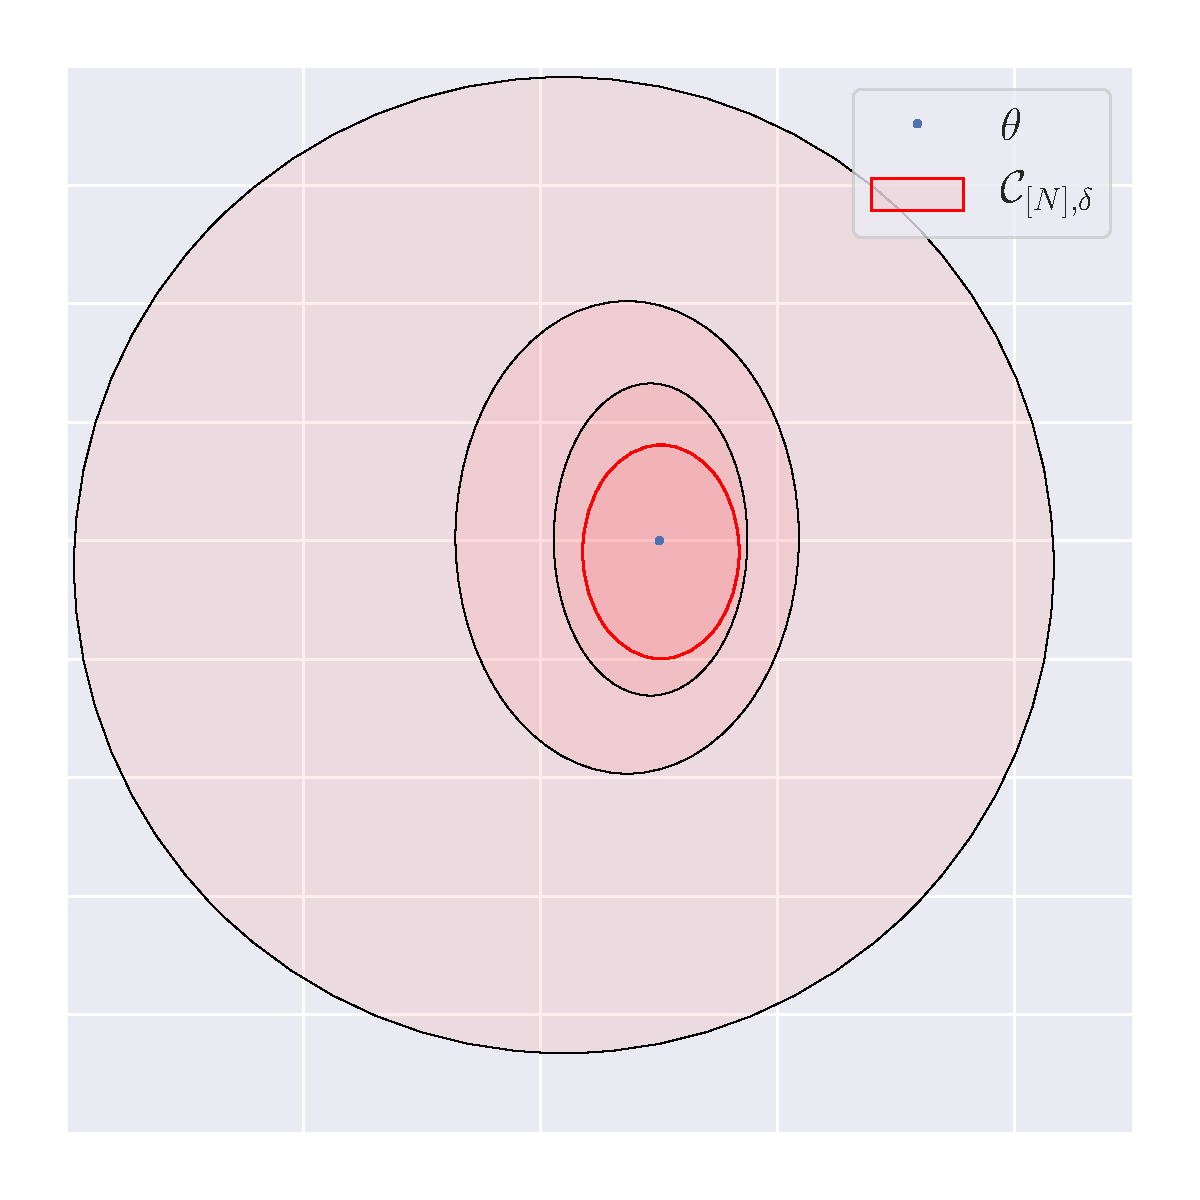
\includegraphics[trim={0 2cm 0 0}, clip, width=0.6\linewidth]{img/ellipsoid}
	\caption{The model estimation procedure, running on the obstacle avoidance problem of \autoref{sec:interval-experiments}. The confidence region $C_{[N],\delta}$ shrinks with the number of samples $N$.}
	\label{fig:estimation}
\end{figure}

\begin{figure}[t]
	\centering
	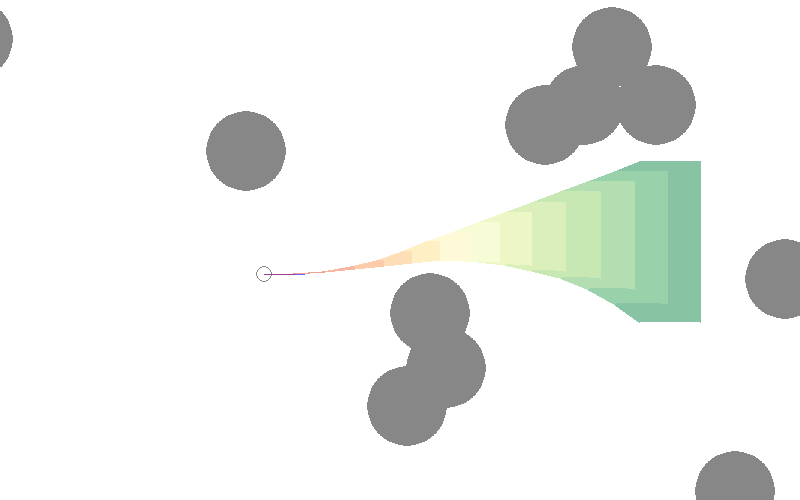
\includegraphics[width=0.8\linewidth]{img/obstacle_small}
	\caption{The state prediction procedure running on the obstacle avoidance problem of \autoref{sec:interval-experiments}. At each time step (red to green), we bound the set of reachable states under model uncertainty \eqref{eq:confidence}}
	\label{fig:prediction}
\end{figure}

In \autoref{sec:estimation}, having observed history of transitions $\cD_{[N]} = \{(x_n, y_n,u_n)\}_{n\in[N]}$, and given a confidence level $\delta\in(0, 1)$, we wish to find a confidence region $\cC_{[N],\delta} \subset \Theta$ as tight as possible and such that it holds that
\begin{align}
\probability{A(\theta)\in \cC_{[N],\delta}} \geq 1-\delta
\label{eq:confidence}
\end{align}
Such regions are illustrated in \autoref{fig:estimation}. Our first contribution extends the work of \citet{Abbasi2011} who provide a confidence ellipsoid for the regularised least-square estimator to our setting of feature matrices, rather than feature vectors.

\paragraph{Robust objective}

At the time step $n=N$, considering the confidence region $\cC_{[N],\delta}$ obtained in the model estimation phase, we formulate our robust control objective
\begin{equation}
\label{eq:robust-control}
\sup_{\bu\in{(\Real^q)}^\Natural} \underbrace{\inf_{\substack{A(\theta) \in \cC_{[N],\delta} \\ \bom\in[\underline{\bom},\overline{\bom}]^\Natural}} \left[\sum_{n=N+1}^\infty \gamma^n R(x_n(\bu,\bom))\right]}_{V^r(\bu)}
\end{equation}
where $\gamma\in(0,1)$ is a discount factor. The rest of the paper tackles the optimisation of \eqref{eq:robust-control}.

\paragraph{State prediction}

Maximin problems such as \eqref{eq:robust-control} are notoriously difficult to solve even in cases such where the reward $R$ has a simple form. With arbitrary functions $R$, we cannot hope to derive a solution in explicit form. Our second contribution is to propose to solve \eqref{eq:robust-control} numerically by adopting a \emph{predict-then-optimise} scheme. In \autoref{sec:prediction}, we aim to derive a \emph{set predictor} $X(t)$ for the system \eqref{eq:dynamics}, illustrated in \autoref{fig:prediction}. This predictor takes the information on the observed current state ${x}_N$, a confidence region $\cC_\delta$ verifying \eqref{eq:confidence}, a planned control sequence $\bu$ and some admissible bounds on the perturbation $[\underline{\omega}(t),\overline{\omega}(t)]$; and outputs a set $X(t)$ that must verify the \emph{inclusion property}
\begin{equation}
\label{eq:inclusion-generic}
x(t)\in X(t),\quad\forall t\geq t_N.
\end{equation}
We leverage recent results from the uncertain system simulation literature to efficiently compute such a predictor.

\paragraph{Robust planning}

Since $R$ is generic, potentially non-smooth and non-convex, solving the optimal -- not to mention the robust -- control objective in the original continuous control space $(\Real^q)^\Natural$ is intractable.
In this work, we choose to approximate the solution of \eqref{eq:robust-control} by optimising over a finite set of \emph{actions} $\cA$. Each action $a\in\cA$ corresponds to the selection of a low-level controller $\pi_a$, that we take affine:
\[u(t) = \pi_a(x(t)) \eqdef -K_a x(t) + u_a.\]
For instance, a tracking a subgoal $x_g$ can be achieved with $\pi_g = K(x_g - x)$. The robust objective \eqref{eq:robust-control} becomes 
\begin{equation}
\label{eq:robust-control-disc}
\sup_{\ba\in{\cA}^\Natural} \underbrace{\inf_{\substack{A(\theta) \in \cC_{[N],\delta} \\ \bom\in[\underline{\bom},\overline{\bom}]^\Natural}} \left[\sum_{n=N+1}^\infty \gamma^n R(x_n(\ba,\bom))\right]}_{V^r(\ba)},
\end{equation}
where $x_n(\ba, \bom)$ stems from \eqref{eq:dynamics} with $u_n = \pi_{a_n}(x_n)$.

In \autoref{sec:control}, facing a sequential decision problem with continuous states and discrete actions, we turn to the literature of tree-based planning algorithms. Our third contribution adapts them to the robust objective \eqref{eq:robust-control-disc} by approximating it with a tractable surrogate $\hat{V}^r$ that exploits the set predictor \eqref{eq:inclusion-generic} to define a pessimistic reward. In our main result, we show that the best surrogate performance achieved during planning is guaranteed to be attained on the true system, and provide an upper bound for the approximation gap and simple regret of our framework in \autoref{thm:control-error}.

The \autoref{alg:full} shows the full integration of the three procedures of estimation, prediction and control. 

\paragraph{Model selection} In \autoref{sec:multi-model}, our forth contribution extends the proposed framework to consider multiple modelling assumptions, while narrowing uncertainty through data-driven model rejection, and still ensuring safety via robust model-selection during planning.

\paragraph{Experiments} Finally, in \autoref{sec:interval-experiments} we demonstrate the applicability of our proposed \autoref{alg:full} in two numerical experiments. First, a simple illustrative example and then, a more challenging simulation for safe autonomous driving.

\begin{algorithm}[tb]
	\caption{Robust Estimation, Prediction and Control}
	\label{alg:full}
%	\begin{algorithmic}
%		\STATE {\bfseries Input:} confidence level $\delta$, structure $(A,\phi)$, reward $R$
%		\STATE $\cD_{[0]}\gets\emptyset,\, \ba_1\gets\emptyset$
%		\FOR{$N = 0,1,2,\dots$} 
%		\STATE $\cC_{[N],\delta} \gets$\textsc{Model Estimation}$(\cD_{[N]})$. \eqref{eq:polytope}
%		\FOR{each planning step $k\in[K]$}
%		\FOR{each action $b\in \cA$}
%		\STATE $[\underline{x}_{n+1}, \overline{x}_{n+1}]\gets$ \textsc{Interval Prediction}(
%		\STATE $\qquad\qquad\qquad\qquad\cC_{[N],\delta}, \ba_kb$). \eqref{eq:interval-predictor}
%		\ENDFOR
%		\STATE $\ba_{k+1}$ $\gets$\textsc{Pessimistic Planning}$($
%		\STATE$\qquad\qquad\underline{R_{n+1}}([\underline{x}_{n+1}, \overline{x}_{n+1}]))$.  \eqref{eq:opd}
%		\ENDFOR
%		\STATE Execute the recommended control $u_{N+1}$, and add the observed transition $(x_{N+1}, y_{N+1}, u_{N+1})$ to $\cD_{[N+1]}$.
%		\ENDFOR
%	\end{algorithmic}
\end{algorithm}

\subsection{Related Work}

\paragraph{Linear-quadratic problems} There is a rich body of literature dedicated to the study of linear systems with quadratic costs, and we focus on those providing non-asymptotic results when the system parameters $A, B$ are unknown. In their seminal work \citet{abbasi-yadkori11a}, consider the problem of cumulative regret minimisation. They follow the \emph{Optimism in the Face of Uncertainty} paradigm from the multi-armed bandit literature, that consists in selecting the best possible dynamics within a high-confidence region while enforcing a controllability constraint, and computing the corresponding optimal control in closed-form by solving a Riccati equation. They show that this procedures achieves a $\tilde{\cO}\left(N^{1/2}\right)$ cumulative regret. \citep{Ibrahimi2013,Faradonbeh2017} adapt these results to the case of sparse dynamics. \citet{Ouyang2017,abeille18a} provide the same result by applying Thomson Sampling rather of optimism to select a dynamical model, and rejection sampling to enforce the controllability constraint. These methods aim at regret minimisation to quickly reduce uncertainty, through information-seeking behaviours. Other works use noise injection for exploration such as \citep{Dean2017,Dean2018}. However, neither optimism and cumulative regret minimisation nor random exploration fit a critical setting, where ensuring safety as a top priority requires instead to consider the pessimistic outcomes.
The work of \citet{Dean2017} is closest to our setting: after an offline estimation phase, where the controls do not aim at regret minimisation, they estimate a simple regret between a robust controller and the optimal performance. Our work mainly differs in that it addresses generic costs and forbids random exploration.

\paragraph{Robust planning}
Robust optimisation with generic costs has also been studied in the context of finite Markov Decision Processes with uncertain parameters by \citet{Iyengar2005}, \citet{Nilim2005} and \citet{Wiesemann2013}. They showed that the main results of Dynamic Programming can be extended to their robust counterparts only when the dynamics ambiguity set verifies a certain rectangularity property, that amounts to an independence assumption between the uncertainty sets of each transition and is related to time-varying uncertainty. Since our setting requires dealing with continuous states and time-invariant uncertainty, these methods do not apply.


\section{Confident model estimation}


\label{sec:estimation}

To derive a confidence region \eqref{eq:confidence} for the dynamical parameters $\theta$, the functional relationship $A(\theta)$ must be specified.
\begin{assumption}[Structure]
	\label{assumpt:structure}
	\begin{leftbar}[assumptionbar]
	There exists a known feature tensor $\phi\in \Real^{d \times p \times p}$ such that for all $\theta\in\Theta$,
	\begin{equation}
	A(\theta) = A + %\theta^\transp \phi \eqdef A + 
	\sum_{i=1}^d \theta_i\phi_i,
	\end{equation}
	where $A,\phi_1,\dots,\phi_d\in\Real^{p\times p}$ are known. For all $n$, we denote $\Phi_n = [\phi_1 x_n \dots \phi_d x_n]\in\Real^{p\times d}$.
	
	We also assume to know a bound $S$ such that $\theta\in[-S,S]^d$.
	\end{leftbar}
\end{assumption}

We abuse notations and define a virtual measurement signal, still denoted $y(t)$, that includes additional known terms
\begin{equation*}
%\label{eq:measurement}
y(t) = \dot{x}(t) + C\nu(t) - A x(t) - Bu(t),
\end{equation*}
to obtain a linear regression system
$
y_n = \Phi_n\theta + \eta_n.
$

\paragraph{Regularised least square} To derive an estimate on $\theta$, we consider the weighted $L_2$-regularised regression problem with weights  $\Sigma_p\in\Real^{p\times p}$ and parameter $\lambda\in\Real^+_*$:
\begin{equation}
\label{eq:regression_min}
\min_{\theta\in\Real^d} \sum_{n=1}^N \|y_n -\Phi_n\theta\|_{\Sigma_p^{-1}}^2 + \lambda\|\theta\|_{}^2.
\end{equation}


The solution can be obtained as

\begin{proposition}[Regularised solution]
	\label{prop:regularized_solution}
	\begin{leftbar}[propositionbar]
	The solution to \eqref{eq:regression_min} is
	\begin{align}
	\label{eq:vector_rls}
	\theta_{N,\lambda} &= G_{N, \lambda}^{-1} \sum_{n=1}^N \Phi_n^\transp \Sigma_p^{-1} y_n,\\
	\label{eq:g_n_lambda}
	\text{where }\quad G_{N, \lambda} &= \sum_{n=1}^N \Phi_{n}^\transp\Sigma_p^{-1}\Phi_{n}  + \lambda I_d \in \Real^{d\times d}.
	\end{align}
	\end{leftbar}
\end{proposition}

Substituting $y_n$ into \eqref{eq:vector_rls} yields the regression error
\begin{align}
\theta_{N,\lambda} - \theta = G_{N, \lambda}^{-1}\sum_{n=1}^N \Phi_n^\transp \Sigma_p^{-1}\eta_n - \lambda G_{N, \lambda}^{-1}\theta.
\end{align}


Depending on the assumption we have over the noise $\eta_n$, we can bound this error in different ways.


\subsection{Bounded noise}

\begin{assumption}[Bounded noise]
	\label{assumpt:bounded-noise}
	\begin{leftbar}[assumptionbar]
	The noise $\eta(t)$ is bounded in $\|\cdot\|_\infty$.
	\end{leftbar}
\end{assumption}

In particular, we denote the coefficient-wise bounds over perturbations as $\underline{\omega}(t) \leq \omega(t) \leq \overline{\omega}(t)$. This is a deterministic assumption, then by Hölder inequality a confidence region $\cC_{[N],0}$ can be derived based on a $L_1$-ball estimate of $\theta$ at time $N$, i.e. a polytope with $2d$ vertices
\begin{equation}
\label{eq:bounded-noise-polytope}
\|\theta_{N,\lambda}\! -\! \theta\|_1\! \leq \! \|G_{N, \lambda}^{-1}\!\sum_{n=1}^N \!\Phi_n^\transp\! \Sigma_p^{-1}\!\|_1\|\eta\|_\infty\! +\!\lambda\|G_{N, \lambda}^{-1}\!\|_1S
\end{equation}

There may be cases where \autoref{assumpt:bounded-noise} does not hold. For instance, when the noise $\eta$ is Gaussian, then $\|\eta\|_\infty=+\infty$ which makes \eqref{eq:bounded-noise-polytope} uninformative. Then, another probabilistic assumption can be made.

\subsection{Sub-Gaussian noise}

\begin{assumption}[Sub-Gaussian Noise]
	\label{assumpt:gaussian-noise}
	\begin{leftbar}[assumptionbar]
	At each time $t\geq0$ the noise $\eta(t)$ is an independent sub-Gaussian noise with covariance proxy $\Sigma_p \in \Real^{p\times p}$:
	\begin{equation*}
	\forall u\in\Real^p,\, \expectedvalue \left[ \exp{\left( u^\transp \eta(t)\right)}\right] \leq \exp{\left( \frac{1}{2} u^\transp \Sigma_p u\right)}.
	\end{equation*}
	\end{leftbar}
\end{assumption}
For instance, it is the case when $\nu$ and $\omega$ are Gaussian noises with covariance matrices $\Sigma_r$ and $\Sigma_s$, with $\Sigma_p \eqdef C\Sigma_r C^\transp + D\Sigma_s D^\transp$. Note that \autoref{assumpt:bounded-noise} implies that $\eta$ is sub-Gaussian with covariance proxy $\Sigma_p=\|\eta\|_\infty I_p$.

\begin{theorem}[Confidence ellipsoid, a matricial version of \citealt{Abbasi2011}]
	\label{thm:confidence_ellipsoid}
	\begin{leftbar}[theorembar]
	Under \autoref{assumpt:gaussian-noise}, it holds with probability at least $1-\delta$ that
	\begin{align}
	\label{eq:confidence-ellipsoid}
	\| \theta_{N,\lambda}  - \theta\|_{G_{N,\lambda}} \leq \beta_N(\delta),
	\end{align}
	with
	\begin{equation}
	\label{eq:beta_n}
	\beta_N(\delta)\eqdef \sqrt{2\ln \left(\frac{\det(G_{N,\lambda})^{1/2}}{\delta\det(\lambda I_d)^{1/2}}\right)}
	+ (\lambda d)^{1/2}S.
	\end{equation}
	\end{leftbar}
\end{theorem}

We can enclose this confidence ellipsoid $\eqref{eq:confidence-ellipsoid}$ into a polytope $C_{[N],\delta}$. For simplicity, we present here a simple but coarse strategy: bound the ellipsoid by its enclosing sphere, and then the sphere by its enclosing hypercube. We obtain
\begin{align}
\label{eq:polytope}
&\cC_{[N],\delta} = \left\{ A_{0}+\sum_{i=1}^{2^d}\alpha_{i}\Delta A_{i}: \alpha\geq 0,  \sum_{i=1}^{2^d}\alpha_{i}=1\right\}
\end{align}
where $A_{0,N} = A + \theta_{N,\lambda}^\transp\phi, \Delta A_{i} = {h_i} \sqrt{\frac{\beta_N(\delta)}{\lambda_{\max}(G_{N,\lambda})}}, h_i\in\{-1,1\}^d$. Another strategy presented in the Supplementary Material produces a much tighter polytope, at the price of an increased computational cost required by the diagonalisation of $G_{N,\lambda}$.

\begin{remark}
	\begin{leftbar}[remarkbar]
	The robust objective \eqref{eq:robust-control} involves bounds $\underline{\omega}(t)\leq \omega(t) \leq \overline{\omega}(t)$ over the possible perturbations we want to protect against. In the unbounded sub-Gaussian noise setting of \autoref{assumpt:gaussian-noise}, we can use the same formulation by deriving local high-confidence bounds that each holds with confidence $\delta_n$. By choosing $\delta_n = \frac{\delta}{n(n+1)}$, the event $\{\forall n, \underline{\omega}(t_n) \leq \omega(t_n) \leq \overline{\omega}(t_n)\}$ holds with probability $1-\delta$.
	\end{leftbar}
\end{remark}

\section{State interval prediction}


\label{sec:prediction}

%To study the inclusion property \eqref{eq:inclusion-generic}, we must start by choosing a set representation $X(t)$. We consider interval prediction, rather than zonotope prediction for instance \citep[e.g.][]{le2012}, for the sake of simplicity of implementation and computational efficiency. We represent an interval as $X(t) = [\underline{x}(t), \overline{x}(t)]\in \Real^p\times \Real^p$, and \eqref{eq:inclusion-generic} becomes
%\begin{equation}
%\label{eq:inclusion-property}
%\underline{x}(t)\leq x(t)\leq\overline{x}(t),\quad\forall t\geq t_N.
%\end{equation} 
%
%A simple solution to \eqref{eq:inclusion-property} is proposed in \citep{Efimov2012}, where, given bounds $\underline{A}\leq A(\theta)\leq\overline{A}$ from $\cC_{[N],\delta}$ they use matrix interval arithmetic to derive the predictor
%\begin{proposition}[Simple predictor of \citealt{Efimov2012}]
%	Assuming that \eqref{eq:confidence} is satisfied for the system \eqref{eq:dynamics}, then the interval predictor
%	\begin{eqnarray}
%	\dot{\underline{x}}(t) & = & \underline{A}^{+}\underline{x}^{+}(t)-\overline{A}^{+}\underline{x}^{-}(t)-\underline{A}^{-}\overline{x}^{+}(t) +\overline{A}^{-}\overline{x}^{-}(t)\nonumber \\
%	&  &+Bu(t) + D^{+}\underline{\omega}(t)-D^{-}\overline{\omega}(t),\label{eq:predictor-naive}\\
%	\dot{\overline{x}}(t) & = & \overline{A}^{+}\overline{x}^{+}(t)-\underline{A}^{+}\overline{x}^{-}(t)-\overline{A}^{-}\underline{x}^{+}(t)+\underline{A}^{-}\underline{x}^{-}(t)\nonumber \\
%	&  &+Bu(t) + D^{+}\overline{\omega}(t)-D^{-}\underline{\omega}(t),\nonumber \\
%	&  & \underline{x}(t_N)=\overline{x}(t_N)={x}(t_N),\nonumber 
%	\end{eqnarray}
%	ensures the inclusion property \eqref{eq:inclusion-property} with confidence level $\delta$.
%\end{proposition}
%
%However, \citet{leurent2019interval} showed that this predictor can have unstable dynamics, even for stable systems, which causes a fast build-up of uncertainty. They proposed an enhanced predictor which exploits the polytopic structure \eqref{eq:polytope} to produce tighter and more stable predictions, at the price of an additional requirement:
%
%\begin{assumption}
%	\label{assumpt:metzler}
%	There exists an orthogonal matrix $Z\in\Real^{p\times p}$ such that $Z^\transp A_0 Z$ is Metzler\footnote{We say that a matrix is Metlzer when all its non-diagonal coefficients are non-negative.}.
%\end{assumption}
%In practice, this assumption is often verified. It is for instance the case whenever $A_0$ is diagonalisable. The similarity transformation of \citep{Efimov2013} provides a method to compute such $Z$ when the system is observable. To simplify the notation, we will further assume that $Z = I_p$. Denote $
%\Delta A_{+}=\sum_{i=1}^{2^d}\Delta A_{i}^{+},\;\Delta A_{-}=\sum_{i=1}^{2^d}\Delta A_{i}^{-}$.
%% The similarity transformation of \citep{Efimov_a2013} provides a method to compute such $P$ whenever there exist $C_1,C_2$ which make $(A(\theta), C_1)$ and $(A_0, C_2)$ observable.
%% Under this assumption, without loss of generality up to a change of basis $x\rightarrow P^{-1}x$ that we do not write for the sake of readability, this assumption is equivalent to considering that $A_0$ itself is Metzler.
%
%\begin{proposition}[Enhanced predictor of \citealt{leurent2019interval}]
%	\label{prop:predictor}
%	Assuming that \eqref{eq:polytope} and \autoref{assumpt:metzler} are satisfied for the system \eqref{eq:dynamics}, then the interval predictor
%	\begin{eqnarray}
%	\dot{\underline{x}}(t) & = & A_{0}\underline{x}(t)-\Delta A_{+}\underline{x}^{-}(t)-\Delta A_{-}\overline{x}^{+}(t)\nonumber \\
%	&  & +Bu(t)+D^{+}\underline{\omega}(t)-D^{-}\overline{\omega}(t),\nonumber\\
%	\dot{\overline{x}}(t) & = & A_{0}\overline{x}(t)+\Delta A_{+}\overline{x}^{+}(t)+\Delta A_{-}\underline{x}^{-}(t) \label{eq:interval-predictor} \\
%	&  & +Bu(t)+D^{+}\overline{\omega}(t)-D^{-}\underline{\omega}(t),\nonumber \\
%	&  & \underline{x}(t_N)=\overline{x}(t_N)={x}(t_N)\nonumber 
%	\end{eqnarray}
%	ensures the inclusion property \eqref{eq:inclusion-property} with confidence level $\delta$..
%\end{proposition}
%
%\begin{figure}[tp]
%	\centering
%	{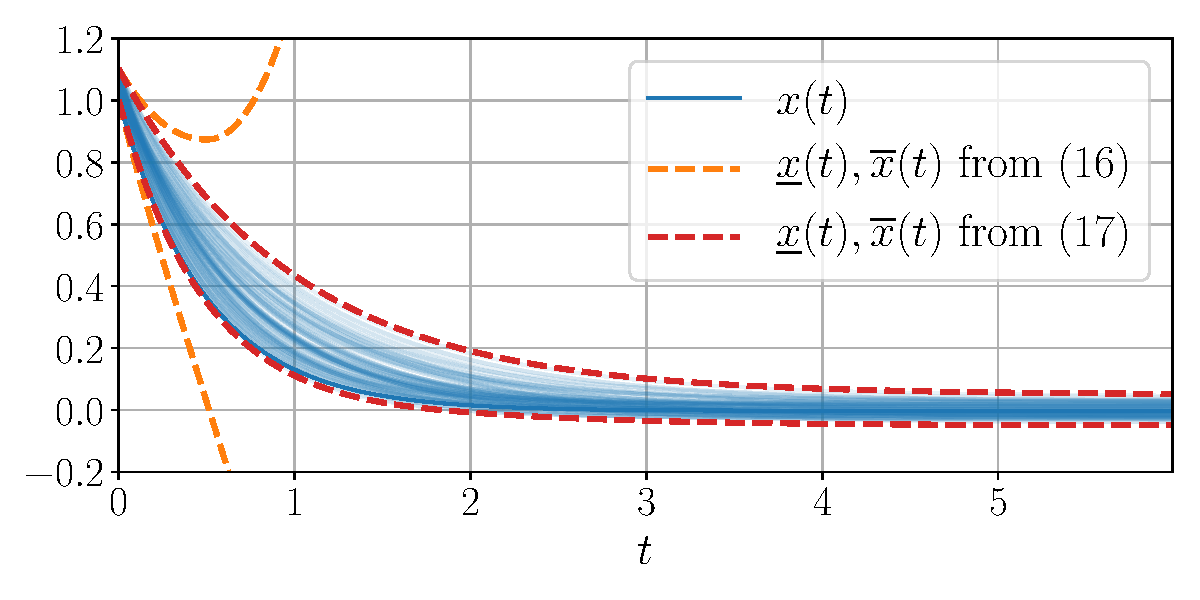
\includegraphics[trim={0 0.6cm 0 0.4cm}, clip, width=\linewidth]{img/interval-predictor}}
%	\vspace{-0.7cm}
%	\caption{Comparison of \eqref{eq:predictor-naive} and \eqref{eq:interval-predictor} for a simple system \\$\dot{x}(t)=-\theta x(t)+\omega(t)$, with $\theta\in[1, 2]$ and $\omega(t) \in [-0.05, 0.05]$.}
%	\label{fig:predictor_example}
%\end{figure}
%
%\autoref{fig:predictor_example} illustrates the difference of stability of the two predictors \eqref{eq:predictor-naive} and \eqref{eq:interval-predictor} with a simple example. It suggests to always prefer \eqref{eq:interval-predictor} whenever \autoref{assumpt:metzler} is verified, and only fallback to \eqref{eq:predictor-naive} as a last resort.



There are plenty of emerging application domains nowadays, where the decision algorithms have to operate in the conditions of a severe uncertainty. To mention a few: the systems biology and control of bioreactors (where it is hard to establish detailed models and it is impossible to isolate and evaluate most of the external to the plant perturbations) and the path planning for self-driving cars (where despite of a large parametric variation of the models, the presence of humans in the loop introduces a lot of imprecision due to their spontaneous reactions). Therefore, the decision procedures need more information, then the estimation, identification and prediction algorithms come to the attention. In most of these applications, even the nominal simplified models are nonlinear, and in order to solve the problem of estimation and control in nonlinear and uncertain systems, a popular approach is based on the Linear Parameter-Varying (LPV) representation of their dynamics \cite{Shamma2012,Marcos_Balas04,Shamma_Cloutier93,Tan97}, since it allows to reduce the problem to the linear context at the price of augmented parametric variation.

In the presence of uncertainty (unknown parameters or/and external disturbances) the design of a conventional estimator or predictor, approaching the ideal value of the state, can be realized under restrictive assumptions only. However, an interval estimation/prediction remains frequently feasible: using input-output information an algorithm evaluates the set of admissible values (interval) for the state at each instant of time \cite{Efimov2016,Raiessi2018}. The interval length must be minimized via a parametric tuning of the system, and it is typically proportional to the size of the model uncertainty \cite{Chebotarev2015}. It is worth stressing that the interval estimation or prediction is not a relaxation of the original problem, in fact it is an improvement since the interval mean value can be used as the state pointwise estimate, while the interval bounds provide a simultaneous accuracy evaluation for given uncertainty.

There are many approaches to design interval/set-membership estimators and predictors \cite{Jaulin02,Kieffer_Walter04,Bernard_Gouze04,Moisan_Bernard_Gouze09}, and this paper focuses on the design based on the monotone systems theory \cite{Bernard_Gouze04,Moisan_Bernard_Gouze09,RVZ10,REZ11,Efimov_a2012}.
In such a way the main difficulty for synthesis consists in ensuring cooperativity of the interval error dynamics by a proper design of the algorithm. As it has been shown in \cite{MazencBernard11,REZ11,Combastel2012}, such a complexity of the design can be handled by applying an additional transformation of coordinates, which maps a stable system into a stable and monotone one. An approach for selection of a constant similarity transformation matrix representing a given interval of matrices to an interval of Metzler matrices (providing monotonicity) has been developed in \cite{Efimov_a2013,Chebotarev2015}. 

The objective of this paper is to propose an interval predictor for linear time-invariant (LTI) and LPV systems. The main difficulty to overcome is the predictor stability, which contrarily to an observer cannot be imposed by a proper design of the gains. An interval inclusion of the uncertain components can be restrictive and transform an initially stable system to an unstable one. In other words, an important problem is to keep the interval predictor stability in the presence of uncertainties and saving the interval inclusion property of the estimates, then an unstable system can definitely enclose the trajectories of a stable one, but at the price of the precision. To solve this problem, first, a generic predictor is proposed for an LPV system, whose estimates can be combined with the interval frequency based estimator presented earlier. To analyze stability of the predictor, which is modeled by a nonlinear Lipschitz dynamics, a novel non-conservative Lyapunov function is developed, whose features can be verified through solution of linear matrix inequalities (LMIs). Second, we revisit the case of LTI models and demonstrate an asymptotic accuracy improvement that can be achieved if an additional information about external signals are given: the admissible interval of frequency spectrum. Finally, the utility of the developed theory is demonstrated on the problem of path planning for a self-driving car by making comparison with earlier results from \cite{Leurent2018}.

The paper is organized as follows. An introduction to the theory of interval estimation for LTI systems is given in Section \ref{sec:Preliminaries}. The problem statement and a motivating example are introduced in Section \ref{sec:Problem-statement}. An improved interval predictor is presented in Section \ref{sec:Main-results}. The asymptotic accuracy is enhanced using frequency based estimation in Section \ref{sec:Frequency}. Application of the developed theory to the problem of path planning for an autonomous vehicle is shown in Section \ref{sec:Examples}.

\subsubsection{Preliminaries}
\label{sec:Preliminaries}

We denote the real numbers  by $\mathbb{R}$, the integers by $\Natural$, $\Real_{+}=\{\tau\in\Real:\tau\ge0\}$ and $\Natural_{+}=\Natural\cap\Real_{+}$. Euclidean norm for a vector $x\in\mathbb{R}^{n}$ will be denoted as $|x|$, and for a measurable and locally essentially bounded input $u:\mathbb{R}_{+}\to\mathbb{R}$ the symbol $||u||_{[t_{0},t_{1}]}$ denotes its $L_{\infty}$ norm
\[
||u||_{[t_{0},t_{1}]}=\text{ess}\sup_{t\in[t_{0},t_{1})}|u(t)|,
\]
if $t_{1}=+\infty$ then we will simply write $||u||$. We will denote as $\mathcal{L}_{\infty}$ the set of all inputs $u$ with the property $||u||<\infty$. 

Denote the sequence of integers $1,...,k$ as $\overline{1,k}$. 

The symbols $I_{n}$, $E_{n\times m}$ and $E_{p}$ denote the identity matrix with dimension $n\times n$, and the matrices with all elements equal 1 with dimensions $n\times m$ and $p\times1$, respectively. The normal basis vectors in $\Real^{n}$ are denoted as $e_{i}=[0\dots0\;1\;\dots0]\tr$ for $i=\overline{1,n}$, where $1$ appears in the $i^{\text{th}}$ position.

For a matrix $A\in\Real^{n\times n}$ the vector of its eigenvalues is denoted as $\lambda(A)$, $||A||_{max}=\max_{i=\overline{1,n},j=\overline{1,n}}|A_{i,j}|$ (the elementwise maximum norm, it is not sub-multiplicative) and $||A||_{2}=\sqrt{\max_{i=\overline{1,n}}\lambda_{i}(A\tr A)}$ (the induced $L_{2}$ matrix norm), the relation $||A||_{max}\le||A||_{2}\le n||A||_{max}$ is satisfied between these norms.

\subsubsection{Interval arithmetic}

For two vectors $x_{1},x_{2}\in\mathbb{R}^{n}$ or matrices $A_{1},A_{2}\in\Real^{n\times n}$, the relations $x_{1}\le x_{2}$ and $A_{1}\le A_{2}$ are understood elementwise. The relation $P\prec0$ ($P\succ0$) means that a symmetric matrix $P\in\Real^{n\times n}$ is negative (positive) definite. Given a matrix $A\in\Real^{m\times n}$, define $A^{+}=\max\{0,A\}$, $A^{-}=A^{+}-A$ (similarly for vectors) and denote the matrix of absolute values of all elements by $|A|=A^{+}+A^{-}$. 
\begin{lemma}
	\textup{\cite{EFRZS12}} \label{lem:interval} Let $x\in\mathbb{R}^{n}$ be a vector variable, $\underline{x}\le x\le\overline{x}$ for some $\underline{x},\overline{x}\in\mathbb{R}^{n}$. 
	
	\textup{(1)} If $A\in\Real^{m\times n}$ is a constant matrix, then
	\begin{equation}
	A^{+}\underline{x}-A^{-}\overline{x}\le Ax\le A^{+}\overline{x}-A^{-}\underline{x}.\label{eq:Interval1}
	\end{equation}
	
	\textup{(2)} If $A\in\Real^{m\times n}$ is a matrix variable and \textup{$\underline{A}\le A\le\overline{A}$} for some $\underline{A},\overline{A}\in\Real^{m\times n}$, then
	\begin{gather}
	\underline{A}^{+}\underline{x}^{+}-\overline{A}^{+}\underline{x}^{-}-\underline{A}^{-}\overline{x}^{+}+\overline{A}^{-}\overline{x}^{-}\leq Ax\label{eq:Interval2}\\
	\leq\overline{A}^{+}\overline{x}^{+}-\underline{A}^{+}\overline{x}^{-}-\overline{A}^{-}\underline{x}^{+}+\underline{A}^{-}\underline{x}^{-}.\nonumber 
	\end{gather}
\end{lemma}
Furthermore, if $-\overline{A}=\underline{A}\le0\le\overline{A}$, then the inequality (\ref{eq:Interval2}) can be simplified: $-\overline{A}(\overline{x}^{+}+\underline{x}^{-})\leq Ax\leq\overline{A}(\overline{x}^{+}+\underline{x}^{-})$.

\subsubsection{Nonnegative systems}

A matrix $A\in\Real^{n\times n}$ is called Hurwitz if all its eigenvalues have negative real parts, it is called Metzler if all its elements outside the main diagonal are nonnegative. Any solution of the linear system
\begin{gather}
\dot{x}(t)=Ax(t)+B\omega(t),\:t\geq0,\label{eq:LTI_syst}\\
y(t)=Cx(t)+D\omega(t),\nonumber 
\end{gather}
with $x(t)\in\Real^{n}$, $y(t)\in\Real^{p}$ and a Metzler matrix $A\in\Real^{n\times n}$, is elementwise nonnegative for all $t\ge0$ provided that $x(0)\ge0$, $\omega:\Real_{+}\to\Real_{+}^{q}$ and $B\in\Real_{+}^{n\times q}$ \cite{FarinaRinaldi2000,Smith95}. The output solution $y(t)$ is nonnegative if $C\in\Real_{+}^{p\times n}$ and $D\in\Real_{+}^{p\times q}$. Such dynamical systems are called cooperative (monotone) or nonnegative if only initial conditions in $\Real_{+}^{n}$ are considered \cite{FarinaRinaldi2000,Smith95}.
\begin{lemma}[\citealt{REZ11}]
	\label{lem:l2}
	\begin{leftbar}[lemmabar]
	Given the matrices $A\in\Real^{n\times n}$, $Y\in\Real^{n\times n}$ and \textup{$C\in\Real^{p\times n}$. }If there is a matrix \textup{$L\in\Real^{n\times p}$} such that the matrices $A-LC$ and $Y$ have the same eigenvalues, then there is a matrix $S\in\Real^{n\times n}$ such that $Y=S(A-LC)S^{-1}$ provided that the pairs $(A-LC,\chi_{1})$ and $(Y,\chi_{2})$ are observable for some $\chi_{1}\in\Real^{1\times n}$, $\chi_{2}\in\Real^{1\times n}$.
	\end{leftbar}
\end{lemma}
This result allows to represent the system \eqref{eq:LTI_syst} in its nonnegative form via a similarity transformation of coordinates.
\begin{lemma}[\citealt{Efimov_a2013}]
	\label{lem:l3}
	\begin{leftbar}[lemmabar]
	Let $D\in\Xi\subset\Real^{n\times n}$ be a matrix variable satisfying the interval constraints $\Xi=\{D\in\Real^{n\times n}:\,D_{a}-\Delta\le D\le D_{a}+\Delta\}$ for some $D_{a}^{\text{T}}=D_{a}\in\Real^{n\times n}$ and $\Delta\in\Real_{+}^{n\times n}$. If for some constant $\mu\in\Real_{+}$ and a diagonal matrix $\Upsilon\in\Real^{n\times n}$ the Metzler matrix $Y=\mu E_{n\times n}-\Upsilon$ has the same eigenvalues as the matrix $D_{a}$, then there is an orthogonal matrix $S\in\Real^{n\times n}$ such that the matrices $S^{\text{T}}DS$ are Metzler for all $D\in\Xi$ provided that $\mu>n||\Delta||_{max}$.\textup{ }
	\end{leftbar}
\end{lemma}
In the last lemma, the existence of similarity transformation is proven for an interval of matrices, \emph{e.g}. in the case of LPV dynamics.

\subsubsection{Problem statement}
\label{sec:Problem-statement}

Consider an LPV system
\begin{equation}
\dot{x}(t)=A(\theta(t))x(t)+Bd(t),\;t\geq0,\label{eq:LPV_syst}
\end{equation}
where $x(t)\in\Real^{n}$ is the state, $\theta(t)\in\Pi\subset\Real^{r}$ is the vector of scheduling parameters with a known set of admissible values $\Pi$, $\theta\in\cL_{\infty}^{r}$; the signal $d:\Real_{+}\to\Real^{m}$ is the external input. The values of the scheduling vector $\theta(t)$ are not available for measurements, and only the set of admissible values $\Pi$ is known. The matrix $B\in\Real^{n\times m}$ is known, the matrix function $A:\Pi\to\Real^{n\times n}$ is locally bounded (continuous) and also known.

The following assumptions will be used in this work.
\begin{assumption}
	\label{ass:a1}
	\begin{leftbar}[assumptionbar]
		In the system \eqref{eq:LPV_syst}, $x\in\cL_{\infty}^{n}$. In addition, $x(0)\in[\underline{x}_{0},\overline{x}_{0}]$ for some known $\underline{x}_{0},\overline{x}_{0}\in\Real^{n}$.
	\end{leftbar}
\end{assumption}

\begin{assumption}
	\label{ass:a2}
	\begin{leftbar}[assumptionbar]
		There exists known signals $\underline{d},\overline{d}\in\cL_{\infty}^{n}$ such that $\underline{d}(t)\leq d(t)\leq\overline{d}(t)$ for all $t\geq0$.
	\end{leftbar}
\end{assumption}
Assumption \ref{ass:a1} means that the system \eqref{eq:LPV_syst} generates stable trajectories with a bounded state $x$ for the applied class of inputs $d$, and the initial conditions $x(0)$ are constrained to belong to a given interval $[\underline{x}_{0},\overline{x}_{0}]$. In Assumption \ref{ass:a2}, it is supposed that the input $d(t)$ belongs to a known bounded interval $[\underline{d}(t),\overline{d}(t)]$ for all $t\in\Real_{+}$, which is the standard hypothesis for the interval estimation \cite{Efimov2016,Raiessi2018}.

Note that since the function $A$ and the set $\Pi$ are known, and $\theta\in\Pi$, then there exist matrices $\underline{A},\overline{A}\in\Real^{n\times n}$, which can be easily computed, such that 
\[
\underline{A}\leq A(\theta)\leq\overline{A},\quad\forall\theta\in\Pi.
\]

\subsubsection{The goal}

The objective of this work is to design an \emph{interval predictor} for the system \eqref{eq:LPV_syst}, which takes the information on the initial conditions $[\underline{x}_{0},\overline{x}_{0}]$, the admissible bounds on the values of the exogenous input $[\underline{d}(t),\overline{d}(t)]$, the information about $A$ and $\Pi$ (\emph{e.g}. the matrices $\underline{A},\overline{A}$, but not the instant value of $\theta(t)$) and generates bounded interval estimates $\underline{x}(t),\overline{x}(t)\in\Real^{n}$ such that
\begin{equation}
\underline{x}(t)\leq x(t)\leq\overline{x}(t),\quad\forall t\geq0.\label{eq:inclusion-property}
\end{equation}

\subsubsection{A motivation example}

Following the result of Lemma \ref{lem:interval}, there is a straightforward solution to the problem used in \cite{Leurent2018}:
\begin{eqnarray}
\dot{\underline{x}}(t) & = & \underline{A}^{+}\underline{x}^{+}(t)-\overline{A}^{+}\underline{x}^{-}(t)-\underline{A}^{-}\overline{x}^{+}(t)  +\overline{A}^{-}\overline{x}^{-}(t)+B^{+}\underline{d}(t)-B^{-}\overline{d}(t),\label{eq:predictor-naive}\\
\dot{\overline{x}}(t) & = & \overline{A}^{+}\overline{x}^{+}(t)-\underline{A}^{+}\overline{x}^{-}(t)-\overline{A}^{-}\underline{x}^{+}(t) +\underline{A}^{-}\underline{x}^{-}(t)+B^{+}\overline{d}(t)-B^{-}\underline{d}(t),\nonumber \\
&  & \underline{x}(0)=\underline{x}_{0},\;\overline{x}(0)=\overline{x}_{0},\nonumber 
\end{eqnarray}
then it is obvious to verify that the relations \eqref{eq:inclusion-property} are satisfied, but the stability analysis of the system \eqref{eq:predictor-naive} is more tricky. Indeed, \eqref{eq:predictor-naive} is a purely nonlinear system (since $\underline{x}^{+}$, $\underline{x}^{-}$, $\overline{x}^{+}$ and $\overline{x}^{-}$ are globally Lipschitz functions of the state $\underline{x}$ and $\overline{x}$), whose robust stability with respect to the bounded external inputs $\underline{d}$ and $\overline{d}$ can be assessed if a suitable Lyapunov function is found. And it is easy to find an example, where the matrices $\underline{A}$ and $\overline{A}$ are stable, but the system \eqref{eq:predictor-naive} is not:
\begin{example*}
	[motivating] Consider a scalar system
	\[
	\dot{x}(t)=-\theta(t)x(t)+d(t),\;t\geq0,
	\]
	where $x(t)\in\Real$ with $x(0)\in[\underline{x}_{0},\overline{x}_{0}]=[1.0, 1.1]$, $\theta(t)\in\Pi=[\underline{\theta},\overline{\theta}]=[0.5,1.5]$ and $d(t)\in[\underline{d},\overline{d}]=[-0.1,0.1]$ for all $t\geq0$. Obviously, assumptions \ref{ass:a1} and \ref{ass:a2} are satisfied, and this uncertain dynamics produces bounded trajectories (to prove this consider a Lyapunov function $V(x)=x^{2}$). Then the interval predictor \eqref{eq:predictor-naive} takes the form
	\begin{eqnarray*}
		\dot{\underline{x}}(t) & = & -\overline{\theta}\overline{x}^{+}(t)+\underline{\theta}\overline{x}^{-}(t)+\underline{d},\\
		\dot{\overline{x}}(t) & = & -\underline{\theta}\underline{x}^{+}(t)+\overline{\theta}\underline{x}^{-}(t)+\overline{d}.
	\end{eqnarray*}
	The results of simulation are shown in Fig. \ref{fig:IP_Direct}. As we can conclude, additional consideration and design are needed to properly solve the posed problem.
	\begin{figure}
		\begin{centering}
			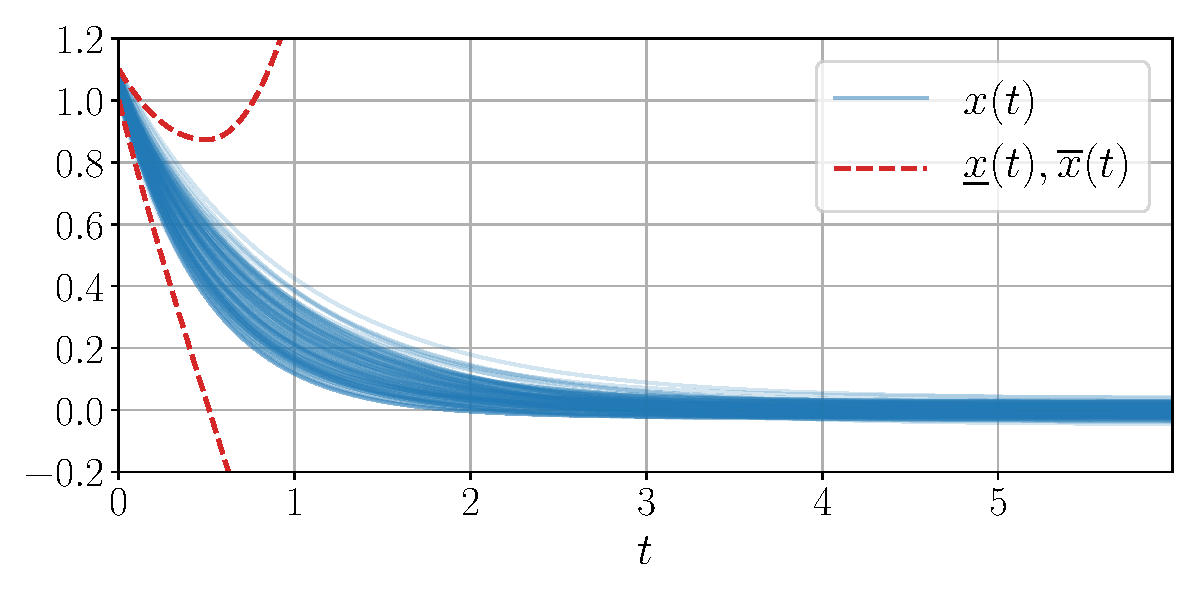
\includegraphics[width=\linewidth]{img/observer}
			\par\end{centering}
		\caption{\label{fig:IP_Direct} The results of prediction by \eqref{eq:predictor-naive}: even in such a simplistic setting, the predictor is unstable and diverges quickly.}
	\end{figure}
\end{example*}

\subsection{Interval predictor design}
\label{sec:Main-results}

Note that, in related papers \cite{AitRami2008,RVZ10,Bolajraf2011,Efimov_a2013,Efimov_tac2013,Chebotarev2015}, various interval observers for LPV systems have been proposed, but in those works the cooperativity and stability of the estimation error dynamics are ensured by a proper selection of observer gains and/or by design of control algorithms, which can be dependent on $\underline{x}$, $\overline{x}$ and guarantee the observer robust stability. For interval predictor there is no such a freedom, then a careful selection of hypotheses has to be made in order to provide a desired solution.
We will additionally assume the following:
\begin{assumption}
	\label{ass:a3}
	\begin{leftbar}[assumptionbar]
	There exist a Metzler matrix $A_{0}\in\Real^{n\times n}$ and matrices $\Delta A_{i}\in\Real^{n\times n}$, $i=\overline{1,N}$ for some $N\in\Natural_{+}$ such that the following relations are satisfied for all $\theta\in\Pi$:
	\begin{gather*}
	A(\theta)=A_{0}+\sum_{i=1}^{N}\lambda_{i}(\theta)\Delta A_{i},\\
	\sum_{i=1}^{N}\lambda_{i}(\theta)=1;\;\lambda_{i}(\theta)\in[0,1],\;i=\overline{1,N}.
	\end{gather*}
	\end{leftbar}
\end{assumption}
Therefore, it is assumed that the matrix $A(\theta)$ for any $\theta\in\Pi$ can be embedded in a polytope defined by $N$ known vertices $\Delta A_{i}$ with the given center $A_{0}$, which admits already useful properties. According to the results of lemmas \ref{lem:l2} and \ref{lem:l3}, the fulfillment of Assumption \ref{ass:a3} can be imposed by applying a properly designed similarity transformation, which maps a matrix (interval of matrices) to a Metzler one. Design of such a transformation is not considered in this work, and we will just suppose in Assumption \ref{ass:a3} that the system \eqref{eq:LPV_syst} has been already put in the right form:
\[
\dot{x}(t)=[A_{0}+\sum_{i=1}^{N}\lambda_{i}(\theta(t))\Delta A_{i}]x(t)+Bd(t).
\]
Denote
\[
\Delta A_{+}=\sum_{i=1}^{N}\Delta A_{i}^{+},\;\Delta A_{-}=\sum_{i=1}^{N}\Delta A_{i}^{-},
\]
then the following interval predictor can be designed:
\begin{theorem}
	\label{thm:main}
	\begin{leftbar}[theorembar]
	Let assumptions \ref{ass:a1}\textendash \ref{ass:a3} be satisfied for the system \eqref{eq:LPV_syst}, then an interval predictor
	\begin{eqnarray}
	\dot{\underline{x}}(t) & = & A_{0}\underline{x}(t)-\Delta A_{+}\underline{x}^{-}(t)-\Delta A_{-}\overline{x}^{+}(t)  +B^{+}\underline{d}(t)-B^{-}\overline{d}(t),\label{eq:interval-predictor}\\
	\dot{\overline{x}}(t) & = & A_{0}\overline{x}(t)+\Delta A_{+}\overline{x}^{+}(t)+\Delta A_{-}\underline{x}^{-}(t)  +B^{+}\overline{d}(t)-B^{-}\underline{d}(t),\nonumber \\
	&  & \underline{x}(0)=\underline{x}_{0},\;\overline{x}(0)=\overline{x}_{0}\nonumber 
	\end{eqnarray}
	ensures the property \eqref{eq:inclusion-property}. If there exist diagonal matrices $P$, $Q$, $Q_{+}$, $Q_{-}$, $Z_{+}$, $Z_{-}$, $\Psi_{+}$, $\Psi_{-}$, $\Psi$, $\Gamma\in\Real^{2n\times2n}$ such that the following LMIs are satisfied:
	\begin{gather*}
	P+\min\{Z_{+},Z_{-}\}>0,\;\Upsilon\preceq0,\;\Gamma>0,\\
	Q+\min\{Q_{+},Q_{-}\}+2\min\{\Psi_{+},\Psi_{-}\}>0,
	\end{gather*}
	where{\footnotesize{}
		\begin{gather*}
		\Upsilon=\left[\begin{array}{cccc}
		\Upsilon_{11} & \Upsilon_{12} & \Upsilon_{13} & P\\
		\Upsilon_{12}^{\top} & \Upsilon_{22} & \Upsilon_{23} & Z_{+}\\
		\Upsilon_{13}^{\top} & \Upsilon_{23}^{\top} & \Upsilon_{33} & Z_{-}\\
		P & Z_{+} & Z_{-} & -\Gamma
		\end{array}\right],\\
		\Upsilon_{11}=\mathcal{A}^{\top}P+P\mathcal{A}+Q,\;\Upsilon_{12}=\mathcal{A}^{\top}Z_{+}+PR_{+}+\Psi_{+},\\
		\Upsilon_{13}=\mathcal{A}^{\top}Z_{-}+PR_{-}+\Psi_{-},\;\Upsilon_{22}=Z_{+}R_{+}+R_{+}^{\top}Z_{+}+Q_{+},\\
		\Upsilon_{23}=Z_{+}R_{-}+R_{+}^{\top}Z_{-}+\Psi,\;\Upsilon_{33}=Z_{-}R_{-}+R_{-}^{\top}Z_{-}+Q_{-},\\
		\mathcal{A}=\left[\begin{array}{cc}
		A_{0} & 0\\
		0 & A_{0}
		\end{array}\right],\;R_{+}=\left[\begin{array}{cc}
		0 & -\Delta A_{-}\\
		0 & \Delta A_{+}
		\end{array}\right],\;R_{-}=\left[\begin{array}{cc}
		\Delta A_{+} & 0\\
		-\Delta A_{-} & 0
		\end{array}\right],
		\end{gather*}
	}then the predictor \eqref{eq:interval-predictor} is input-to-state stable with respect to the inputs $\underline{d}$, $\overline{d}$.
\end{leftbar}
\end{theorem}
Note the requirement that the matrix $P$ has to be diagonal is not restrictive, since for a Metzler matrix $\mathcal{A}$, its stability is equivalent to existence of a diagonal solution $P$ of the Lyapunov equation $\mathcal{A}^{\top}P+P\mathcal{A}\prec0$ \cite{FarinaRinaldi2000}.
\begin{proof}
	First, let us demonstrate \eqref{eq:inclusion-property}, to this end note that
	\[
	-\Delta A_{i}^{-}\leq\lambda_{i}\Delta A_{i}=\lambda_{i}\Delta A_{i}^{+}-\lambda_{i}\Delta A_{i}^{-}\leq\Delta A_{i}^{+}
	\]
	for any $\lambda_{i}\in[0,1],$ then using Lemma \ref{lem:interval} we obtain
	\[
	-\Delta A_{i}^{+}\underline{x}^{-}-\Delta A_{i}^{-}\overline{x}^{+}\leq\lambda_{i}\Delta A_{i}x\leq\Delta A_{i}^{+}\overline{x}^{+}+\Delta A_{i}^{-}\underline{x}^{-}
	\]
	provided that $\underline{x}\leq x\leq\overline{x}$. Hence,
	\[
	-\Delta A_{+}\underline{x}^{-}-\Delta A_{-}\overline{x}^{+}\leq\sum_{i=1}^{N}\lambda_{i}\Delta A_{i}x\leq\Delta A_{+}\overline{x}^{+}+\Delta A_{-}\underline{x}^{-}
	\]
	and introducing usual interval estimation errors $\underline{e}=x-\underline{x}$ and $\overline{e}=\overline{x}-x$ and calculating their dynamics we get:
	\begin{eqnarray*}
		\dot{\underline{e}}(t) & = & A_{0}\underline{e}(t)+\underline{r}_{1}(t)+\underline{r}_{2}(t),\\
		\dot{\overline{e}}(t) & = & A_{0}\overline{e}(t)+\overline{r}_{1}(t)+\overline{r}_{2}(t),
	\end{eqnarray*}
	where
	\begin{gather*}
	\underline{r}_{1}=\sum_{i=1}^{N}\lambda_{i}\Delta A_{i}x+\Delta A_{+}\underline{x}^{-}+\Delta A_{-}\overline{x}^{+},\\
	\underline{r}_{2}=Bd-B^{+}\underline{d}+B^{-}\overline{d},\\
	\overline{r}_{1}=\Delta A_{+}\overline{x}^{+}+\Delta A_{-}\underline{x}^{-}-\sum_{i=1}^{N}\lambda_{i}\Delta A_{i}x,\\
	\overline{r}_{2}=B^{+}\overline{d}-B^{-}\underline{d}-Bd.
	\end{gather*}
	Non-negativity or $\underline{r}_{2}$ and $\overline{r}_{2}$ follows from Assumption \ref{ass:a2} and Lemma \ref{lem:interval}. The signals $\underline{r}_{1}$ and $\overline{r}_{1}$ are also nonnegative provided that \eqref{eq:inclusion-property} holds and due to the calculations above. Note that the relations \eqref{eq:inclusion-property} are satisfied for $t=0$ by construction and Assumption \ref{ass:a1}, then since the matrix $A_{0}$ is Metzler by Assumption \ref{ass:a3}, we have that $\dot{\underline{e}}_{i}(0)\in\Real_{+}^{n}$ or $\dot{\overline{e}}_{i}(0)\in\Real_{+}^{n}$ provided that $e_{i}(0)=0$ or $e_{i}(0)=0$, respectively, for any $i=\overline{1,n}$ (the error cannot become negative). Next, repeating these arguments it is possible to show that $\underline{e}(t)\geq0$ and $\overline{e}(t)\geq0$ for all $t\geq0$ \cite{Smith95}, which confirms the relations \eqref{eq:inclusion-property}.
	
	Second, let us consider the stability of \eqref{eq:interval-predictor}, and for this purpose define the extended state vector as $X=[\underline{x}^{\top}\;\;\overline{x}^{\top}]^{\top}$, whose dynamics admit the differential equation
	\[
	\dot{X}(t)=\mathcal{A}X(t)+R_{+}X^{+}(t)-R_{-}X^{-}(t)+\delta(t),
	\]
	where
	\begin{gather*}
	\delta(t)=\left[\begin{array}{cc}
	-B^{-} & B^{+}\\
	B^{+} & -B^{-}
	\end{array}\right]\left[\begin{array}{c}
	\overline{d}(t)\\
	\underline{d}(t)
	\end{array}\right]
	\end{gather*}
	is a bounded input vector, whose norm is proportional to $\underline{d}$,
	$\overline{d}$. Consider a candidate Lyapunov function
	\begin{gather*}
	V(X)=X^{\top}PX+X{}^{\top}Z_{+}X^{+}-X^{\top}Z_{-}X^{-}\\
	=\sum_{k=1}^{2n}P_{k,k}X_{k}^{2}+(Z_{+})_{k,k}X_{k}X_{k}^{+}-(Z_{-})_{k,k}X_{k}X_{k}^{-}\\
	=\sum_{k=1}^{2n}P_{k,k}X_{k}^{2}+(Z_{+})_{k,k}|X_{k}|X_{k}^{+}+(Z_{-})_{k,k}|X_{k}|X_{k}^{-},
	\end{gather*}
	which is positive definite provided that
	\[
	P+\min\{Z_{+},Z_{-}\}>0,
	\]
	and whose derivative for the system dynamics takes the form
	\begin{gather*}
	\dot{V}=2\dot{X}^{\top}PX+2\dot{X}^{\top}Z_{+}X^{+}-2\dot{X}^{\top}Z_{-}X^{-}\\
	=\left[\begin{array}{c}
	X\\
	X^{+}\\
	-X^{-}\\
	\delta
	\end{array}\right]^{\top}\Upsilon\left[\begin{array}{c}
	X\\
	X^{+}\\
	-X^{-}\\
	\delta
	\end{array}\right]-X^{\top}QX-(X^{+})^{\top}Q_{+}X^{+}\\
	-(X^{-})^{\top}Q_{-}X^{-}-2(X^{+})^{\top}\Psi X^{-}-2(X^{+})^{\top}\Psi_{+}X\\
	-2(-X^{-})^{\top}\Psi_{-}X+\delta^{\top}\Gamma\delta.
	\end{gather*}
	Note that
	\begin{gather*}
	(X^{+})^{\top}\Psi X^{-}=0,\\
	(X^{+})^{\top}\Psi_{+}X\geq0,\;(-X^{-})^{\top}\Psi_{-}X\geq0
	\end{gather*}
	for any diagonal matrix $\Psi$ and
	\[
	\Psi_{+}\geq0,\;\Psi_{-}\geq0.
	\]
	Hence, if $\Upsilon\preceq0$, as it is assumed in the theorem, we obtain that
	\begin{eqnarray*}
		\dot{V} & \leq & -X^{\top}QX-(X^{+})^{\top}Q_{+}X^{+}-(X^{-})^{\top}Q_{-}X^{-}\\
		&  & -2(X^{+})^{\top}\Psi_{+}X-2(-X^{-})^{\top}\Psi_{-}X+\delta^{\top}\Gamma\delta\\
		& \leq & -X^{\top}\Omega X+\delta^{\top}\Gamma\delta,
	\end{eqnarray*}
	where
	\[
	\Omega=Q+\min\{Q_{+},Q_{-}\}+2\min\{\Psi_{+},\Psi_{-}\}>0
	\]
	is a diagonal matrix. The substantiated properties of $V$ and its derivative imply that \eqref{eq:interval-predictor} is input-to-state stable \cite{Khalil2002} with respect to the input $\delta$ (or, by its definition, with respect to $(\underline{d},\overline{d})$).
\end{proof}
\begin{remark}
	\begin{leftbar}[remarkbar]
	The LMIs of the above theorem are not conservative, since the restriction on positive definiteness of involved matrix variables is not imposed on all of them separately, but on their combinations:
	\begin{gather*}
	P+\min\{Z_{+},Z_{-}\}>0,\;\Gamma>0,\\
	Q+\min\{Q_{+},Q_{-}\}+2\min\{\Psi_{+},\Psi_{-}\}>0,
	\end{gather*}
	then some of them can be sign-indefinite or negative-definite ensuring the fulfillment of the last inequality
	$
	\Upsilon\preceq0.
	$
	\end{leftbar}
\end{remark}

\begin{remark}
	\begin{leftbar}[remarkbar]
	Assume that $-\underline{d}=\overline{d}=const\ne0$ and the conditions of Theorem \ref{thm:main} are satisfied, then asymptotically $\underline{x}$ and $\overline{x}$ are negative and positive, respectively. Therefore, the dynamics of \eqref{eq:interval-predictor} takes the form for sufficiently high values of $t\geq0$:
	\begin{eqnarray*}
		\dot{\underline{x}}(t) & = & (A_{0}-\Delta A_{+})\underline{x}(t)-\Delta A_{-}\overline{x}(t)\\
		&  & +B^{+}\underline{d}-B^{-}\overline{d},\\
		\dot{\overline{x}}(t) & = & (A_{0}+\Delta A_{+})\overline{x}(t)+\Delta A_{-}\underline{x}(t)\\
		&  & +B^{+}\overline{d}-B^{-}\underline{d},
	\end{eqnarray*}
	which is a linear system
	\begin{eqnarray}
	\label{eq:linear-asympt}
	\dot{X}(t) & = & \left[\begin{array}{cc}
	A_{0}-\Delta A_{+} & -\Delta A_{-}\\
	\Delta A_{-} & A_{0}+\Delta A_{+}
	\end{array}\right]X(t)\\
	&  & +\left[\begin{array}{cc}
	-B^{-} & B^{+}\\
	B^{+} & -B^{-}
	\end{array}\right]\left[\begin{array}{c}
	\overline{d}\\
	\underline{d}
	\end{array}\right],
	\end{eqnarray}
	where as before $X=[\underline{x}^{\top}\;\;\overline{x}^{\top}]^{\top}$.
	\end{leftbar}
\end{remark}
\begin{example*}
	[motivating, continue] Let us apply the predictor \eqref{eq:interval-predictor}
	to the motivation example:
	\begin{eqnarray*}
		\dot{\underline{x}}(t) & = & -\overline{\theta}\underline{x}(t)-(\overline{\theta}-\underline{\theta})\underline{x}^{-}(t)+\underline{d},\\
		\dot{\overline{x}}(t) & = & -\overline{\theta}\overline{x}(t)+(\overline{\theta}-\underline{\theta})\overline{x}^{+}(t)+\overline{d},
	\end{eqnarray*}
	where $A_{0}=-\overline{\theta}$ is chosen, then $\Delta A_{+}=\overline{\theta}-\underline{\theta}$, $\Delta A_{-}=0$ and all conditions of Theorem \ref{thm:main} are verified. The results of simulation are shown in Fig.~\ref{fig:IP_New}. As we can see the new predictor generates very reasonable and bounded estimates. 
	\begin{figure}
		\begin{centering}
			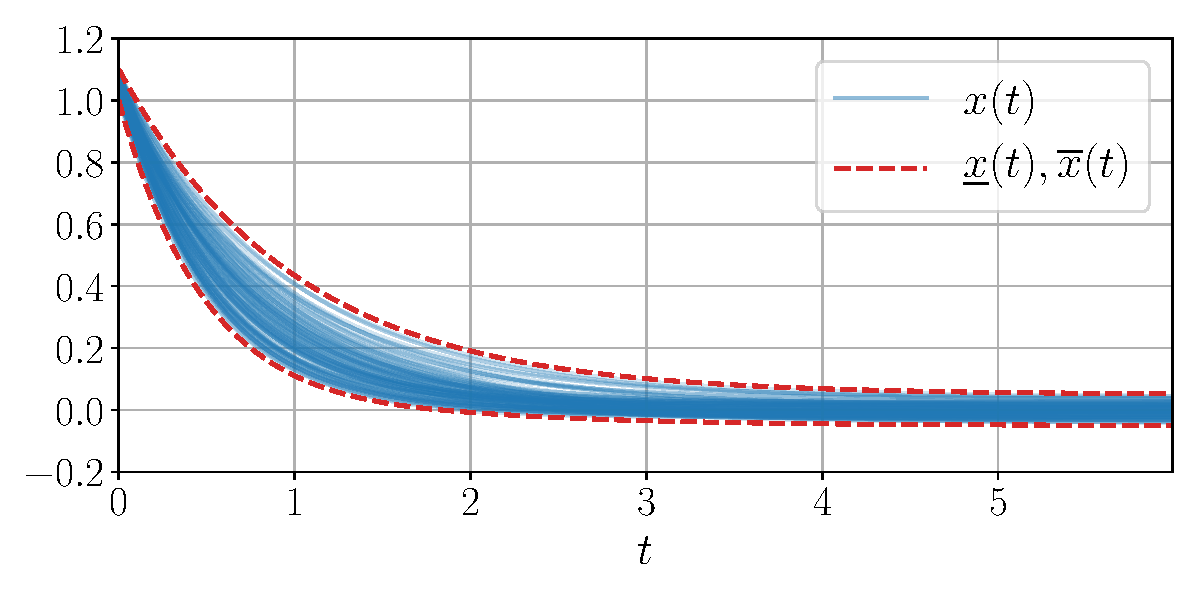
\includegraphics[width=\linewidth]{img/predictor}
			\par\end{centering}
		\caption{\label{fig:IP_New} The results of prediction by \eqref{eq:interval-predictor}: the new predictor is stable and produces tight bounds.}
	\end{figure}
\end{example*}


\subsection{Frequency based interval estimation}
\label{sec:Frequency}
The domain of convergence of the linear system \eqref{eq:linear-asympt}, and hence of \eqref{eq:interval-predictor}, can be tightened under an additional hypothesis that $d(t)$ has a known and bounded frequency spectrum.
Assume that there exist two signals $\underline{\omega},\overline{\omega}:\Real_{+}\to\Real^{q}$ and two vectors $\underline{x}_{0},\overline{x}_{0}\in\Real^{n}$ such that
\begin{gather*}
\underline{\omega}(t)\leq\omega(t)\leq\overline{\omega}(t),\quad\forall t\geq0,\\
\underline{x}_{0}\leq x(0)\leq\overline{x}_{0},
\end{gather*} and there is a matrix $L\in\Real^{n\times p}$ such that $A-LC$ is Hurwitz and Metzler, then an interval observer for the system \eqref{eq:LTI_syst} can be written as follows \cite{REZ11}:
\begin{eqnarray}
\dot{\underline{x}}(t) & = & (A-LC)\underline{x}(t)+Ly(t)\nonumber \\
&  & +(B-LD)^{+}\underline{\omega}(t)-(B-LD)^{-}\overline{\omega}(t),\nonumber \\
\dot{\overline{x}}(t) & = & (A-LC)\overline{x}(t)+Ly(t)\label{eq:IO_LTI}\\
&  & +(B-LD)^{+}\overline{\omega}(t)-(B-LD)^{-}\underline{\omega}(t),\nonumber \\
&  & \underline{x}(0)=\underline{x}_{0},\;\overline{x}(0)=\overline{x}_{0},\nonumber 
\end{eqnarray}
guaranteeing the desired interval relations
\[
\underline{x}(t)\leq x(t)\leq\overline{x}(t),\quad\forall t\geq0.
\]
This solution uses only information about amplitude of the external input $\omega$, and its precision can be largely improved if we assume that there is also information about admissible frequency spectrum in $\omega$:
\begin{lemma}
	\label{lem:IntFreq}
	\begin{leftbar}[lemmabar]
	Let there exist $s_{1},s_{2}\in\Natural_{+}$ and $T,W>0$
	such that
	\[
	\omega(t)=a_{0}+\sum_{s=s_{1}}^{s_{2}}a_{s}\sin\left(\frac{2\pi s}{T}t+\phi_{s}\right),
	\]
	for some $a_{0},a_{s},\phi_{s}\in\Real$ with $s=\overline{s_{1},s_{2}}$ and $||\omega||\leq W$. Then for any $x(0)\in\Real^{n}$ in \eqref{eq:LTI_syst} and any $\epsilon>0$ there exists $\tau>0$ such that
	\[
	|x_{i}(t)|\leq\sup_{w\in[\frac{2\pi}{T}s_{1},\frac{2\pi}{T}s_{2}]}|e_{i}(jwI_{n}-A)^{-1}BE_{q}|W+\epsilon\quad\forall t\geq\tau,
	\]
	where $j$ corresponds to the imaginary unit, provided that the matrix $A$ is Hurwitz.
	\end{leftbar}
\end{lemma}
\begin{proof}
	The solution of the system \eqref{eq:LTI_syst} can be written as follows:
	\[
	x(t)=e^{At}x(0)+\int_{0}^{t}e^{A(t-\sigma)}B\omega(\sigma)d\sigma,
	\]
	where the first term ($e^{At}x(0)$) is converging asymptotically to zero since the matrix $A$ is Hurwitz by hypothesis. And in order to estimate the second term, the Bode magnitude plot can be used, which provides the asymptotic amplitude of the state for the given frequency input. Under the introduced hypotheses, the frequency of the input lies in the interval $[\frac{2\pi}{T}s_{1},\frac{2\pi}{T}s_{2}]$ and the amplitude is upper-bounded by $W$, then there exist constants $\tau>0$ and $\epsilon>0$, related with $x(0)$, such that the claim of the lemma is true.
\end{proof}
The interval observer \eqref{eq:IO_LTI}, if we assume that $\overline{\omega}(t)=-\underline{\omega}(t)=WE_{q}$ and $L=0$, asymptotically will converge to the interval $[-|e_{i}A{}^{-1}BE_{q}|W,|e_{i}A{}^{-1}BE_{q}|W]$ (that corresponds to the result of Lemma \ref{lem:IntFreq} with $s_{1}=s_{2}=0$), which is the estimate from Bode plot given for the frequency $0$, and it is a well-known fact that for many stable systems the Bode magnitude plot is a decreasing function of the frequency. Therefore, if the information about frequency spectrum is known and it is separated from zero, then the asymptotic interval accuracy can be significantly improved. Of course, Lemma \ref{lem:IntFreq} can be applied iteratively for a decreasing sequence of $\epsilon>0$ and an increasing one in $\tau>0$.
\begin{example*}
	Let us illustrate these conclusions on a simple example:
	\begin{gather*}
	A=\left[\begin{array}{cc}
	-1 & 1\\
	0.1 & -1
	\end{array}\right],\;B=\left[\begin{array}{c}
	-2\\
	1
	\end{array}\right],\;L=0,\\
	\overline{\omega}(t)=-\underline{\omega}(t)=1,\\
	\overline{x}_{0}=[2\;1]\tr,\;\underline{x}_{0}=[-1\;-2]\tr.
	\end{gather*}
	And assume that
	$
	\omega(t)=\omega_0\sin(st+\phi_0),\;s=7,
	$
	then the system trajectories and intervals are shown in Fig. \ref{fig:IntFreq}. 
	\begin{figure}
		\begin{centering}
			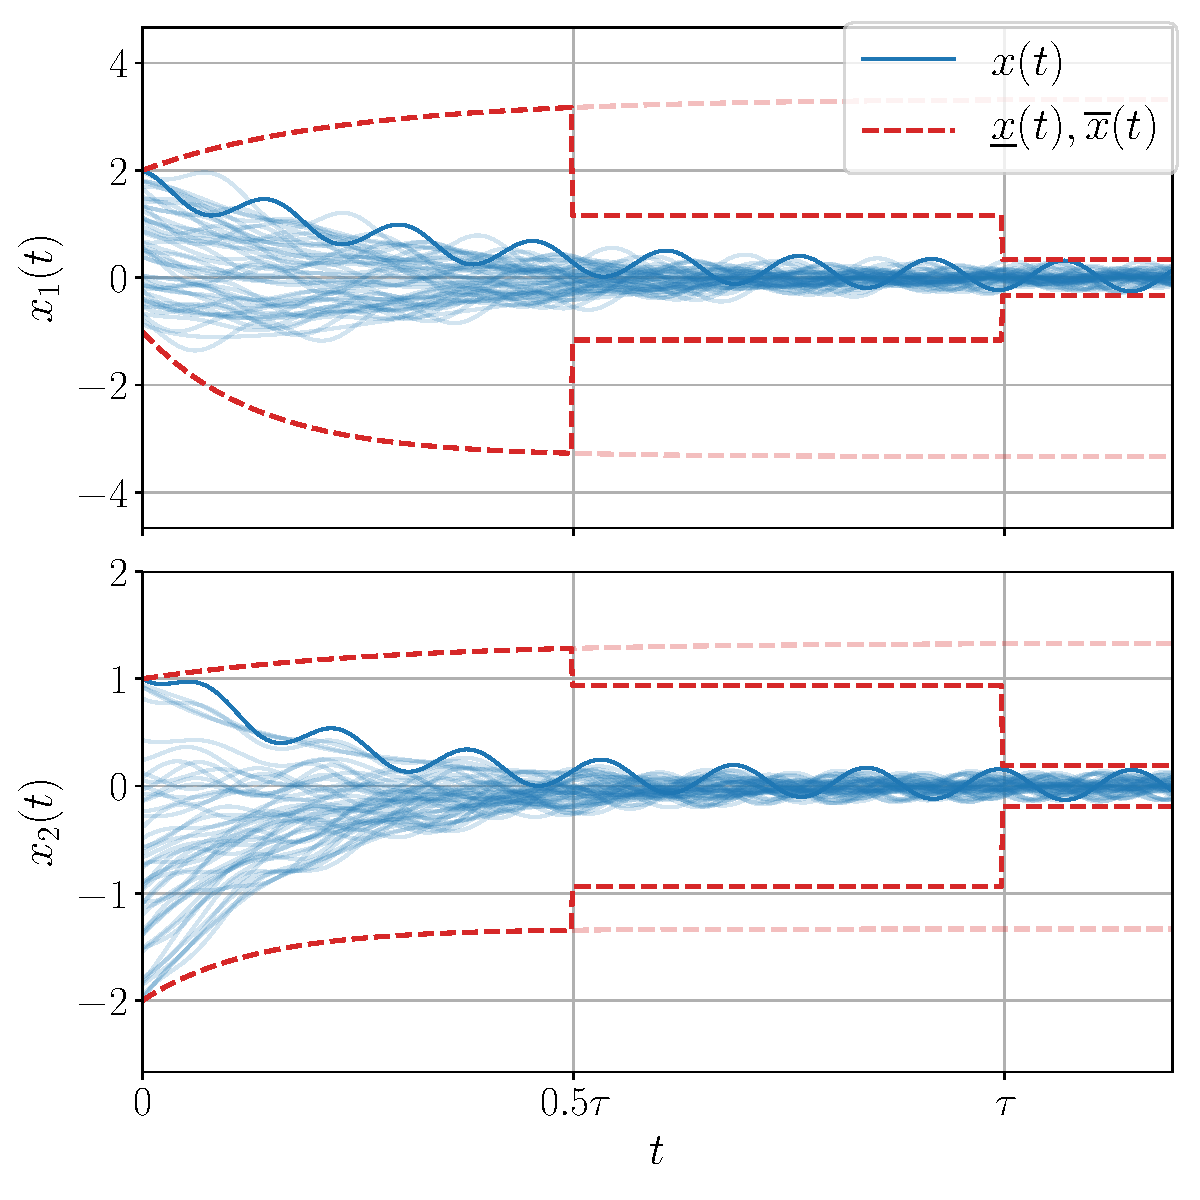
\includegraphics[width=\linewidth]{img/asymptotic}
			\par\end{centering}
		\caption{\label{fig:IntFreq} The results of prediction for different values
			of the frequency. Taking $\tau=\frac{4}{\min_{i=\overline{1,n}}|\lambda_{i}(A)|}=5.85$ and $\epsilon=0.05,$ the trajectories of the interval observer \eqref{eq:IO_LTI} are presented for $t\leq0.5\tau$, and as we can conclude, these estimates are rather conservative. Next, for $t\in[0.5\tau,\tau]$ the estimates given in Lemma \ref{lem:IntFreq} for the case $s_{1}=s_{2}=0$ are shown, which are already more accurate. Finally, for $t\geq\tau$ the estimates of Lemma \ref{lem:IntFreq} are presented for $s_{1}=s_{2}=s$, which demonstrate a definite improvement. }
	\end{figure}
\end{example*}

\subsection{Prediction for a self-driving vehicle}
\label{sec:Examples}
We consider the problem of safe decision-making for autonomous highway driving \cite{highway-env}. The videos and source code of all experiments are available\footnote{\href{https://eleurent.github.io/interval-prediction/}{https://eleurent.github.io/interval-prediction/}}.

An autonomous vehicle is driving on a highway populated with $N$ other agents, and uses Model Predictive Control to plan a sequence of decisions. To that end, it relies on parametrized dynamical model for each agent to predict the future trajectory of each traffic participant: $$\dot{z}_i=f_i(Z,\theta_i),\;i=\overline{1,N},$$ where $f_i$ are described below, $z_i\in\Real^4$ is the state of an agent, $Z = [z_1,\dots,z_N]^\top\in\Real^{4N}$ and $\theta_i\in\Real^5$ is the corresponding vector of unknown parameters. Crucially, this system describes the couplings and interactions between vehicles, so that the autonomous agent can properly anticipate their reactions. 
However, we assume that we do not have access to the true values of the behavioural parameters $\theta=[\theta_1,\dots,\theta_N]^\top$; instead, we merely know that these parameters lie in a set of admissible values $\Pi\subset\Real^{5N}$. In order to act safely in the face of uncertainty, we follow the framework of robust decision-making: the agent must consider all the possible trajectories in the space of $Z$ that each vehicle can follow in order to take its decisions. In this work, we focus on how to compute these trajectory enclosures through interval prediction.

\subsubsection{LPV formulation}

The system presented in \Cref{chapter:3} is non-linear and must be cast into the LPV form. We approximate the non-linearities induced by the trigonometric operators through equilibrium linearisation around $y_i=y_{L_i}$ and $\psi_i=\psi_{L_i}$.

This yields the following longitudinal dynamics:
\begin{align*}
\dot{x}_i &= v_i,\\
\dot v_i &= \theta_{i,1} (v_0 - v_i) + \theta_{i,2} (v_{f_i} - v_i) + \theta_{i,3}(x_{f_i} - x_i - d_0 - v_i T),
\end{align*}
where $\theta_{i,2}$ and $\theta_{i,3}$ are set to $0$ whenever the corresponding features are not active.

It can be rewritten in the form $$\dot{Z} = A(\theta)(Z-Z_c) + d.$$ For example, in the case of two vehicles only,
\begin{equation*}
Z = \begin{bmatrix}
x_i \\
x_{f_i} \\
v_i \\
v_{f_i} \\
\end{bmatrix}
,\quad
Z_c = \begin{bmatrix}
-d_0-v_0 T \\
0 \\
v_0\\
v_0 \\
\end{bmatrix}
,\quad
d = \begin{bmatrix}
v_0 \\
v_0 \\
0\\
0\\
\end{bmatrix}
\end{equation*}

\begin{equation*}
A(\theta)
=
\begin{blockarray}{ccccc}
& i & f_i & i & f_i \\
\begin{block}{c[cccc]}
i & 0 & 0 & 1 & 0 \\
f_i & 0 & 0 & 0 & 1 \\
i & -\theta_{i,3} & \theta_{i,3} & -\theta_{i,1}-\theta_{i,2}-\theta_{i,3} & \theta_{i,2} \\
f_i & 0 & 0 & 0 & -\theta_{f_i,1} \\
\end{block}
\end{blockarray}
\end{equation*}

The lateral dynamics are in a similar form:
\begin{equation*}
\begin{bmatrix}
\dot{y}_i \\
\dot{\psi}_i \\
\end{bmatrix}
=
\begin{bmatrix}
0 & v_i \\
-\frac{\theta_{i,4} \theta_{i,5}}{v_i} & -\theta_{i,5}
\end{bmatrix}
\begin{bmatrix}
y_i - y_{L_i} \\
\psi_i - \psi_{L_i}
\end{bmatrix}
+
\begin{bmatrix}
v_i\psi_{L_i} \\
0
\end{bmatrix}
\end{equation*}
Here, the dependency in $v_i$ is seen as an uncertain parametric dependency, \emph{i.e.} $\theta_{i,6}=v_i$, with constant bounds assumed for $v_i$ using an overset of the longitudinal interval predictor.

\subsubsection{Change of coordinates}
In both cases, the obtained polytope centre $A_0$ is non-Metzler.
We use lemmas \ref{lem:l2} and \ref{lem:l3} to compute a similarity transformation of coordinates. Precisely, we ensure that the polytope is chosen so that its centre $A_0$ is diagonalisable having real eigenvalues, and perform an eigendecomposition to compute its change of basis matrix $S$. The transformed system $Z'=S^{-1}(Z-Z_c)$ verifies Assumption~\ref{ass:a3} as required to apply the interval predictor of Theorem~\ref{thm:main}. Finally, the obtained predictor is transformed back to the original coordinates $Z$ by using the interval arithmetic of Lemma~\ref{lem:interval}.

\subsubsection{Results}

\begin{figure}
	\begin{center}
	\begin{subfigure}[b]{0.8\linewidth}
		\centering
		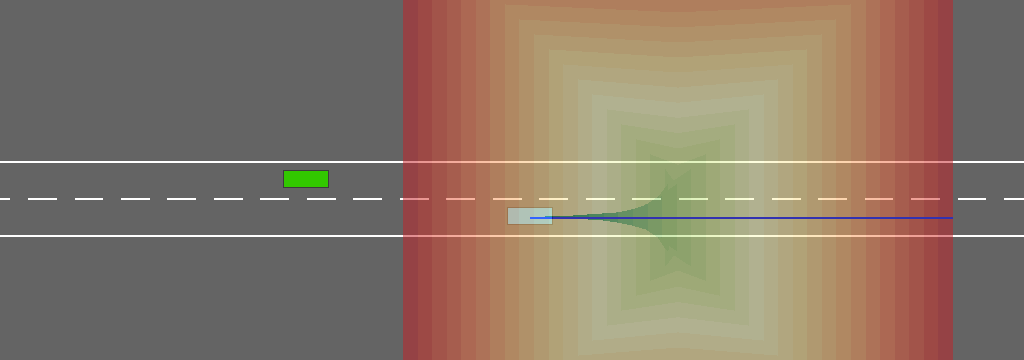
\includegraphics[width=0.7\textwidth]{img/driving_observer.png}
		\caption{The naive predictor \eqref{eq:predictor-naive} quickly diverges}
		\label{sub:hw-a}
	\end{subfigure}
	\begin{subfigure}[b]{0.8\linewidth}
		\centering
		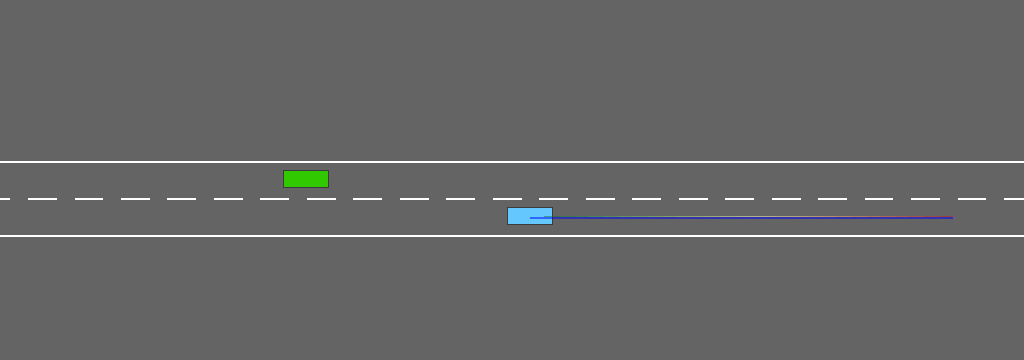
\includegraphics[width=0.7\textwidth]{img/driving_predictor.png}
		\caption{The proposed predictor \eqref{eq:interval-predictor} remains stable}
		\label{sub:hw-b}
	\end{subfigure}
	\begin{subfigure}[b]{0.8\linewidth}
		\centering
		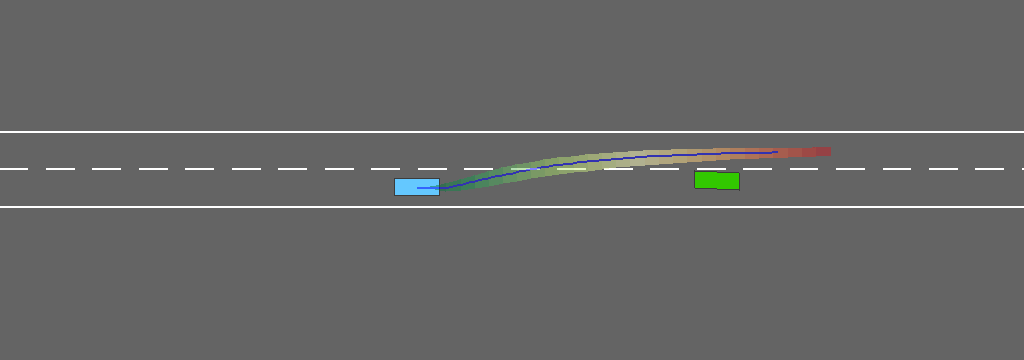
\includegraphics[width=0.7\textwidth]{img/lane_change_predictor.png}
		\caption{Prediction during a lane change maneuver}
		\label{sub:hw-c}
	\end{subfigure}
	\begin{subfigure}[b]{0.8\linewidth}
		\centering
		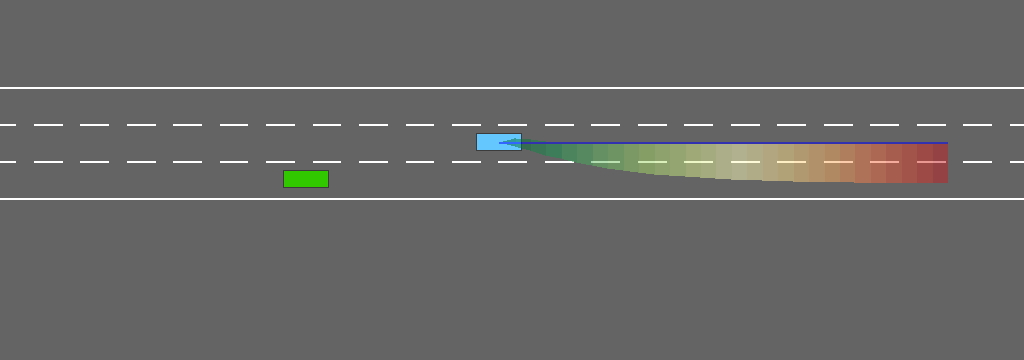
\includegraphics[width=0.7\textwidth]{img/overtake.png}
		\caption{Prediction with uncertainty in the followed lane $L_i$}
		\label{sub:hw-d}
	\end{subfigure}
	\end{center}
	\caption{State intervals obtained by the two methods in different conditions.}
	\label{fig:highway}
\end{figure}


We show the resulting intervals in Fig.~\ref{fig:highway}. The target vehicle with uncertain behaviour is in blue, while the ego-vehicle is in green. Its trajectory interval is computed over a duration of two seconds and represented by an area filled with a colour gradient representing time. The ground-truth trajectory is shown in blue. In Fig.~\ref{sub:hw-a}, we observe that the direct predictor \eqref{eq:predictor-naive} is unstable and quickly diverges to cover the whole road, thus hindering any sensible decision-making. In \cite{Leurent2018}, they had to circumvent this issue by subdividing $\Pi$ and $[\underline{Z}, \overline{Z}]$ to reduce the initial overestimations and merely delay the divergence \cite{Adrot2003}, at the price of a heavy computational load. In stark contrast, we see in Fig.~\ref{sub:hw-b} that the novel predictor \eqref{eq:interval-predictor} is very stable even over long horizons, which allows the ego-vehicle to plan an overtaking maneuver. Until then, there was little uncertainty in the predicted trajectory for the target vehicle was isolated, but as the ego-vehicle cuts into its lane in Fig.~\ref{sub:hw-c}, we start seeing the  effects of uncertain interactions between the two vehicles, in both longitudinal and lateral directions. Our framework is quite flexible in representing different assumptions on the admissible behaviours. For instance, we show in Fig.~\ref{sub:hw-d} a simulation in which we model a right-hand traffic where drivers are expected to keep to the rightmost lane. In such a situation, it is reasonable to assume that in the absence of any obstacle in front, a vehicle driving on the middle lane will either stay there or return to the right lane, but has no incentive to change to the left-lane. This simple assumption on $L_i$ can easily be incorporated in the interval predictor, and enables the emergence of a realistic behaviour when running the robust decision-making procedure: the ego-vehicle cannot pass another vehicle by its right side, and can only overtake it by its left side. These behaviours displaying safe reasoning under uncertainty are showcased in the attached videos.

\subsection*{Conclusion}

The prediction problem for uncertain LPV systems is solved by designing an interval predictor, which is described by nonlinear differential equations, and whose stability is evaluated using a new Lyapunov function. The corresponding robust stability conditions are expressed in terms of LMIs. An approach is presented to improve the asymptotic accuracy of interval estimation or prediction in LTI systems provided that the exogenous inputs have a known spectrum of frequencies. The proficiency of the methods is demonstrated in application to a problem of safe motion planning for a self-driving car.



\section{Robust stabilization and constraint satisfaction}


Our goal is to design a robust control that stabilizes \eqref{eq:dynamics},
\eqref{eq:outputs} at a vicinity of the origin under Assumption \ref{assu:main}
such that
\begin{equation}
x(t)\in\X,\;u(t)\in\U\quad\forall t\geq0,\label{eq:constraints}
\end{equation}
where $[\underline{x}_{0},\overline{x}_{0}]\subset\X\subset\Real^{p}$
and $\U\subset\Real^{q}$ are given bounded constraint sets for the
state and the control, respectively.


\subsection{Stabilizing control for \eqref{eq:predictor-naive} and \eqref{eq:interval-predictor}}

Note that both interval predictors, \eqref{eq:predictor-naive} and
\eqref{eq:interval-predictor}, admit a representation in the form (we use the
time argument $t=s$ in this subsection)
\begin{equation}
\dot{\xi}(t)=\cA_{0}\xi(t)+\cA_{1}\xi^{+}(t)+\cA_{2}\xi^{-}(t)+\cB u(t)+\delta(t),\label{eq:predictor}
\end{equation}
where $\xi(t)=[\underline{x}^{\top}(t)\;\overline{x}^{\top}(t)]^{\top}\in\Real^{2p}$
is the extended state vector of the predictors,
\[
\delta(t)=\left[\begin{array}{cc}
D^{+} & -D^{-}\\
-D^{-} & D^{+}
\end{array}\right]\left[\begin{array}{c}
\underline{\omega}(t)\\
\overline{\omega}(t)
\end{array}\right]\in\Real^{2p}
\]
is the external known input, $\cB=[B^{\top}\;B^{\top}]^{\top}$, 
\[
\cA_{0}=0,\;\cA_{1}=\left[\begin{array}{cc}
\underline{A}^{+} & -\underline{A}^{-}\\
-\overline{A}^{-} & \overline{A}^{+}
\end{array}\right],\;\cA_{2}=\left[\begin{array}{cc}
-\overline{A}^{+} & \overline{A}^{-}\\
\underline{A}^{-} & -\underline{A}^{+}
\end{array}\right]
\]
for \eqref{eq:predictor-naive} and
\[
\cA_{0}=\left[\begin{array}{cc}
A_{0} & 0\\
0 & A_{0}
\end{array}\right],\;\cA_{1}=\left[\begin{array}{cc}
0 & -\Delta A_{-}\\
0 & \Delta A_{+}
\end{array}\right],\;\cA_{2}=\left[\begin{array}{cc}
-\Delta A_{+} & 0\\
\Delta A_{-} & 0
\end{array}\right]
\]
for \eqref{eq:interval-predictor}. Note that \eqref{eq:predictor}
is a nonlinear system due to the presence of globally Lipschitz nonlinearities
$\xi^{+}(t)$ and $\xi^{-}(t)$. 

Due to \eqref{eq:inclusion-generic}, the boundedness of $\xi(t)$
implies the same property of $x(t)$. Therefore, in order to regulate
\eqref{eq:dynamics} it is required to design a state feedback $u(t)$
minimizing the asymptotic amplitude of the state $\xi(t)$ for given
input $\delta(t)$ \cite{Efimov2013a}. In other words, it is necessary
to design a control $u(t)$ that input-to-state stabilizes \eqref{eq:predictor}.
It is proposed to look for such a control in the form
\begin{equation}
u(t)=K_{0}\xi(t)+K_{1}\xi^{+}(t)+K_{2}\xi^{-}(t)+S\delta(t),\label{eq:control_pr}
\end{equation}
where $K_{0},K_{1},K_{2}\in\Real^{q\times2p}$ and $S\in\Real^{q\times2p}$
are the gains to be designed (\eqref{eq:control_pr} contains a nonlinear
feedback). The selection of $S$ is simple, it has to minimize the
norm of $\cB S+I_{2p}$, and it can be made independently of $K_{0},K_{1},K_{2}$.
Therefore, denoting $\tilde{\delta}(t)=(\cB S+I_{2p})\delta(t)$ the
closed-loop system \eqref{eq:predictor}, \eqref{eq:control_pr} takes
the form:
\begin{equation}
\dot{\xi}(t)=\cD_{0}\xi(t)+\cD_{1}\xi^{+}(t)+\cD_{2}\xi^{-}(t)+\tilde{\delta}(t),\label{eq:closed-loop_pr}
\end{equation}
where $\cD_{i}=\cA_{i}+\cB K_{i}$ for $i\in[3]$, and the restrictions,
which the gains $K_{0},K_{1},K_{2}$ have to respect, are given below:
\begin{theorem}
	\begin{leftbar}[theorembar]
	\label{thm:ISS_pr} If there exist diagonal matrices $P$, $Q$, $Q_{+}$,
	$Q_{-}$, $Z_{+}$, $Z_{-}$, $\Psi_{+}$, $\Psi_{-}$, $\Psi$, $\Gamma\in\Real^{2p\times2p}$
	such that the following linear matrix inequalities are satisfied:
	\begin{gather*}
	P+\min\{Z_{+},Z_{-}\}>0,\;\Upsilon\preceq0,\;\Gamma>0,\\
	Q+\min\{Q_{+},Q_{-}\}+2\min\{\Psi_{+},\Psi_{-}\}>0,
	\end{gather*}
	where
	\begin{gather*}
	\Upsilon=\left[\begin{array}{cccc}
	\Upsilon_{11} & \Upsilon_{12} & \Upsilon_{13} & P\\
	\Upsilon_{12}^{\top} & \Upsilon_{22} & \Upsilon_{23} & Z_{+}\\
	\Upsilon_{13}^{\top} & \Upsilon_{23}^{\top} & \Upsilon_{33} & -Z_{-}\\
	P & Z_{+} & -Z_{-} & -\Gamma
	\end{array}\right],\\
	\Upsilon_{11}=\cD_{0}^{\top}P+P\cD_{0}+Q,\;\Upsilon_{12}=\cD_{0}^{\top}Z_{+}+P\cD_{1}+\Psi_{+},\\
	\Upsilon_{13}=P\cD_{2}-\cD_{0}^{\top}Z_{-}-\Psi_{-},\;\Upsilon_{22}=Z_{+}\cD_{1}+\cD_{1}^{\top}Z_{+}+Q_{+},\\
	\Upsilon_{23}=Z_{+}\cD_{2}-\cD_{1}^{\top}Z_{-}+\Psi,\;\Upsilon_{33}=-Z_{-}\cD_{2}-\cD_{2}^{\top}Z_{-}+Q_{-},
	\end{gather*}
	then \eqref{eq:closed-loop_pr} is input-to-state stable with respect
	to $\underline{\omega},\overline{\omega}$.
	\end{leftbar}
\end{theorem}
Note that the requirement that the matrix $P$ has to be diagonal is not
restrictive, since for a Metzler matrix $\cD_{0}$ (the case of \eqref{eq:predictor-naive}
and \eqref{eq:interval-predictor}), its stability is equivalent to
existence of a diagonal solution $P$ of the Lyapunov equation $\cD_{0}^{\top}P+P\cD_{0}\prec0$
\cite{Positive}.
\begin{proof}
	Consider a candidate Lyapunov function
	\begin{gather*}
	V(\xi)=\xi^{\top}P\xi+\xi{}^{\top}Z_{+}\xi^{+}-\xi^{\top}Z_{-}\xi^{-}\\
	=\sum_{k=1}^{2p}P_{k,k}\xi_{k}^{2}+(Z_{+})_{k,k}\xi_{k}\xi_{k}^{+}-(Z_{-})_{k,k}\xi_{k}\xi_{k}^{-}\\
	=\sum_{k=1}^{2p}P_{k,k}\xi_{k}^{2}+(Z_{+})_{k,k}|\xi_{k}|\xi_{k}^{+}+(Z_{-})_{k,k}|\xi_{k}|\xi_{k}^{-},
	\end{gather*}
	which is positive definite provided that
	\[
	P+\min\{Z_{+},Z_{-}\}>0
	\]
	since all terms in $V$ are quadratic-like, and whose derivative for
	the system \eqref{eq:closed-loop_pr} dynamics takes the form
	\begin{gather*}
	\dot{V}=2\dot{\xi}^{\top}P\xi+2\dot{\xi}^{\top}Z_{+}\xi^{+}-2\dot{\xi}^{\top}Z_{-}\xi^{-}\\
	=\left[\begin{array}{c}
	\xi\\
	\xi^{+}\\
	\xi^{-}\\
	\tilde{\delta}
	\end{array}\right]^{\top}\Upsilon\left[\begin{array}{c}
	\xi\\
	\xi^{+}\\
	\xi^{-}\\
	\tilde{\delta}
	\end{array}\right]-\xi^{\top}Q\xi-(\xi^{+})^{\top}Q_{+}\xi^{+}\\
	-(\xi^{-})^{\top}Q_{-}\xi^{-}-2(\xi^{+})^{\top}\Psi\xi^{-}-2(\xi^{+})^{\top}\Psi_{+}\xi\\
	-2(-\xi^{-})^{\top}\Psi_{-}\xi+\tilde{\delta}^{\top}\Gamma\tilde{\delta}.
	\end{gather*}
	Note that
	\begin{gather*}
	(\xi^{+})^{\top}\Psi\xi^{-}=0,\\
	(\xi^{+})^{\top}\Psi_{+}\xi\geq0,\;(-\xi^{-})^{\top}\Psi_{-}\xi\geq0
	\end{gather*}
	for any diagonal matrix $\Psi$ and $\Psi_{+}\geq0$, $\Psi_{-}\geq0$.
	Hence, if $\Upsilon\preceq0$, as it is assumed in the theorem, we
	obtain that
	\begin{eqnarray*}
		\dot{V} & \leq & -\xi^{\top}Q\xi-(\xi^{+})^{\top}Q_{+}\xi^{+}-(\xi^{-})^{\top}Q_{-}\xi^{-}\\
		&  & -2(\xi^{+})^{\top}\Psi_{+}\xi-2(-\xi^{-})^{\top}\Psi_{-}\xi+\tilde{\delta}^{\top}\Gamma\tilde{\delta}\\
		& \leq & -\xi^{\top}\Omega\xi+\tilde{\delta}^{\top}\Gamma\tilde{\delta},
	\end{eqnarray*}
	\[
	\text{where }\Omega=Q+\min\{Q_{+},Q_{-}\}+2\min\{\Psi_{+},\Psi_{-}\}>0
	\]
	is a diagonal matrix. The substantiated properties of $V$ and its
	derivative imply that \eqref{eq:closed-loop_pr} is input-to-state
	stable \cite{Sontag:01:Springer,Dashkovskiy:11:AiT} with respect
	to the input $\tilde{\delta}$ (or, by its definition, with respect
	to $(\underline{\omega},\overline{\omega})$).
\end{proof}
Following the proof of Theorem \ref{thm:ISS_pr}, for all $\xi\in\Real^{2p}$,
\[
\xi^{\top}(P+\min\{Z_{+},Z_{-}\})\xi\leq V(\xi)\leq\xi^{\top}(P+Z_{+}^{+}+Z_{-}^{+})\xi,
\]
then
\[
\dot{V}\leq-\alpha V+\tilde{\delta}^{\top}\Gamma\tilde{\delta}
\]
for all $\xi,\tilde{\delta}\in\Real^{2p}$, where
\[
\alpha=\min_{i\in[2p]}\lambda_{i}\left(\Omega(P+Z_{+}^{+}+Z_{-}^{+})^{-1}\right),
\]
and we can define the set (recall that the signal $\tilde{\delta}(t)$
is known for all $t\geq0$)
\begin{equation}
\X_{f}=\{\xi\in\Real^{2p}:V(\xi)\leq\alpha^{-1}\sup_{t\geq0}|\tilde{\delta}^{\top}(t)\Gamma\tilde{\delta}(t)|\},\label{eq:X_f}
\end{equation}
as the set that asymptotically attracts all trajectories in \eqref{eq:closed-loop_pr}.

The conditions of Theorem \ref{thm:ISS_pr} assume that the control
gains $K_{0},K_{1},K_{2}$ are given, let us find these gains as solutions
of linear matrix inequalities:
\begin{corollary}
	\begin{leftbar}[corollarybar]
	If there exist diagonal matrices $P$, $\tilde{Q}$, $\tilde{Q}_{+}$,
	$\tilde{Q}_{-}$, $Z_{+}$, $Z_{-}$, $\tilde{\Psi}_{+}$, $\tilde{\Psi}_{-}$,
	$\tilde{\Psi}$, $\Gamma\in\Real^{2p\times2p}$ and matrices $U_{0},U_{1},U_{2}\in\Real^{q\times2p}$
	such that the following linear matrix inequalities are satisfied:
	\begin{gather*}
	P>0,\;Z_{+}>0,\;Z_{-}>0,\;\Pi\preceq0,\;\Gamma>0,\\
	\tilde{Q}+\min\{\tilde{Q}_{+},\tilde{Q}_{-}\}+2\min\{\tilde{\Psi}_{+},\tilde{\Psi}_{-}\}>0,
	\end{gather*}
	where
	\begin{gather*}
	\Pi=\left[\begin{array}{cccc}
	\Pi_{11} & \Pi_{12} & \Pi_{13} & I\\
	\Pi_{12}^{\top} & \Pi_{22} & \Pi_{23} & I\\
	\Pi_{13}^{\top} & \Pi_{23}^{\top} & \Pi_{33} & -I\\
	I & I & -I & -\Gamma
	\end{array}\right],\\
	\Pi_{11}=P^{-1}\cA_{0}^{\top}+\cA_{0}P^{-1}+U_{0}^{\top}\cB^{\top}+\cB U_{0}+\tilde{Q},\\
	\Pi_{12}=\cA_{1}Z_{+}^{-1}+\cB U_{1}+P^{-1}\cA_{0}^{\top}+U_{0}^{\top}\cB^{\top}+\tilde{\Psi}_{+},\\
	\Pi_{13}=\cA_{2}Z_{-}^{-1}+\cB U_{2}-P^{-1}\cA_{0}^{\top}-U_{0}^{\top}\cB^{\top}-\tilde{\Psi}_{-},\\
	\Pi_{22}=Z_{+}^{-1}\cA_{1}^{\top}+\cA_{1}Z_{+}^{-1}+U_{1}^{\top}\cB^{\top}+\cB U_{1}+\tilde{Q}_{+},\\
	\Pi_{23}=\cA_{2}Z_{-}^{-1}+\cB U_{2}-Z_{+}^{-1}\cA_{1}^{\top}-U_{1}^{\top}\cB^{\top}+\tilde{\Psi},\\
	\Pi_{33}=\tilde{Q}_{-}-Z_{-}^{-1}\cA_{2}^{\top}-\cA_{2}Z_{-}^{-1}-U_{2}^{\top}\cB^{\top}-\cB U_{2},
	\end{gather*}
	then \eqref{eq:closed-loop_pr} for $K_{0}=U_{0}P$, $K_{1}=U_{1}Z_{+}$
	and $K_{2}=U_{2}Z_{-}$ is input-to-state stable with respect to the
	inputs $\underline{\omega},\overline{\omega}$.
	\end{leftbar}
\end{corollary}
\begin{proof}
	Note that the conditions $P>0$, $Z_{+}>0$, $Z_{-}>0$ imply $P+\min\{Z_{+},Z_{-}\}>0$,
	and 
	\[
	\Upsilon=\left[\begin{array}{cccc}
	P & 0 & 0 & 0\\
	0 & Z_{+} & 0 & 0\\
	0 & 0 & Z_{-} & 0\\
	0 & 0 & 0 & I_{2p}
	\end{array}\right]\Pi\left[\begin{array}{cccc}
	P & 0 & 0 & 0\\
	0 & Z_{+} & 0 & 0\\
	0 & 0 & Z_{-} & 0\\
	0 & 0 & 0 & I_{2p}
	\end{array}\right]
	\]
	under substitution $U_{0}=K_{0}P^{-1}$, $U_{1}=K_{1}Z_{+}^{-1}$,
	$U_{2}=K_{2}Z_{-}^{-1}$, $\tilde{Q}=P^{-1}QP^{-1}$, $\tilde{Q}_{+}=Z_{+}^{-1}Q_{+}Z_{+}^{-1}$,
	$\tilde{Q}_{-}=Z_{-}^{-1}Q_{-}Z_{-}^{-1}$, $\tilde{\Psi}=Z_{-}^{-1}\Psi Z_{+}^{-1}$,
	$\tilde{\Psi}_{+}=P^{-1}\Psi_{+}Z_{+}^{-1}$ and $\tilde{\Psi}_{-}=P^{-1}\Psi_{-}Z_{-}^{-1}$.
	Hence, $\Upsilon\preceq0$ provided that $\Pi\preceq0$. The inequalities
	$\tilde{Q}+\min\{\tilde{Q}_{+},\tilde{Q}_{-}\}+2\min\{\tilde{\Psi}_{+},\tilde{\Psi}_{-}\}>0$
	and $Q+\min\{Q_{+},Q_{-}\}+2\min\{\Psi_{+},\Psi_{-}\}>0$ are equivalent
	due to the diagonal structure of all matrices. Therefore, under introduced
	restrictions all conditions of Theorem \ref{thm:ISS_pr} are verified
	for $K_{0}=U_{0}P$, $K_{1}=U_{1}Z_{+}$ and $K_{2}=U_{2}Z_{-}$.
\end{proof}
The requirements imposed on $P,Z_{+},Z_{-}$ in this corollary are
more restrictive than the conditions of Theorem \ref{thm:ISS_pr},
but it allows the gains $K_{0},K_{1},K_{2}$ to be efficiently calculated.

Under conditions of Theorem \ref{thm:ISS_pr}, the control \eqref{eq:control_pr}
ensures stabilization of the predictor \eqref{eq:predictor} (\emph{i.e}.,
\eqref{eq:predictor-naive} or \eqref{eq:interval-predictor}) in
a vicinity $\X_{f}$ of the origin. The size of the vicinity is proportional
to the system \eqref{eq:dynamics} uncertainty (it can be optimized
by the choice of $K_{0},K_{1},K_{2}$), and due to \eqref{eq:inclusion-generic},
it implies that the system \eqref{eq:dynamics} also will reach a
neighborhood of the origin under the control \eqref{eq:control_pr}.
Hence, the posed control problem would be solved provided that \eqref{eq:constraints}
holds. In order to ensure the robust constraint satisfaction we
consider an MPC design in the next section.

\subsection{\label{sec:control} Robust Control}

For brevity, the results of this section are given for the predictor
\eqref{eq:interval-predictor} only (and the case of \eqref{eq:predictor-naive}
can be considered by skipping Assumption \ref{assu:metzler} in the
formulation). We need the following hypothesis in this section:
\begin{assumption}
	\begin{leftbar}[assumptionbar]
	\label{assu:ctrl} There exist $K_{0},K_{1},K_{2}\in\Real^{q\times2p}$
	satisfying the conditions of Theorem \ref{thm:ISS_pr} for the matrices
	$A_{0}$ and $\Delta A_{i}$ with $i\in[2d]$ calculated in \eqref{eq:polytope}
	for $\hat{\Theta}(t)=\Theta$, and
	\[
	\X_{f}\subset\X^{2},
	\]
	where the corresponding set $\X_{f}$ is given in \eqref{eq:X_f},
	and
	\[
	K_{0}\xi+K_{1}\xi^{+}+K_{2}\xi^{-}+S\delta(t)\in\U
	\]
	for any $\xi\in\X_{f}$ and $t\geq0$.
	\end{leftbar}
\end{assumption}
These properties guarantee that there exists a control \eqref{eq:control_pr}
that can be always applied to stabilize the predictor \eqref{eq:interval-predictor}
(the worst-case estimate set $\Theta$ is used to calculate the system
matrices) and into the set $\X_{f}$ the restrictions \eqref{eq:constraints}
also hold for such a control. Define $T>0$ and $\tau\in(0,T)$ as the interval of prediction and
the application time for MPC, \emph{i.e}., at each $t\geq0$ to design
input $u(t)$, an optimal control problem is solved on the interval
$[t,t+T]$, and this optimal control problem is resolved again
after $\tau$ units of time (on the interval $[t,t+\tau)$ the obtained
optimal control is applied). Denote $t_{i}=i\tau$ for $i\in\Natural_{+}$,
then the developed MPC algorithm can be formalized as follows for
any $t_{i}\geq0$:
\begin{enumerate}
	\item Take $\hat{\Theta}(t_{i})$ from \eqref{eq:set_LS} and calculate
	the matrices $A_{0}$ and $\Delta A_{i}$ with $i\in[2d]$ for \eqref{eq:polytope}.
	\item Find
	\begin{gather}
	\cU=\text{argmin}_{u:[t_{i},t_{i}+T]\to\Real^{q}}\xi^{\top}(t_{i}+T)W_{1}\xi(t_{i}+T)\label{eq:OCP}\\
	+\int_{t_{i}}^{t_{i}+T}\xi^{\top}(s)W_{2}\xi(s)+u^{\top}(s)W_{3}u(s)ds,\nonumber 
	\end{gather}
	where $W_{i}\in\Real^{2p\times2p}$ are given positive definite symmetric
	matrices, such that the following constraints are satisfied: 
	\begin{enumerate}
		\item $\xi:[t_{i},t_{i}+T]\to\Real^{2p}$ is a solution of \eqref{eq:interval-predictor}
		with $t=t_{i}$ and additionally (to counteract the influence of big
		measurement perturbations)
		\begin{align}
		[\underline{x}&(t_{i}),\overline{x}(t_{i})]=\label{eq:update}\\
		&\begin{cases}
		[y_{1}(t_{i})-\underline{\nu}_{1}(t_{i}),y_{1}(t_{i})+\overline{\nu}_{1}(t_{i})] & i=0\\
		\quad\cap[\underline{x}_{0},\overline{x}_{0}];\\{}
		[y_{1}(t_{i})-\underline{\nu}_{1}(t_{i}),y_{1}(t_{i})+\overline{\nu}_{1}(t_{i})] & i\geq1\\
		\quad\cap[\underline{x}(t_{i-1}+\tau),\overline{x}(t_{i-1}+\tau)],
		\end{cases}\nonumber
		\end{align}
		where $(\underline{x}^{\top}(t_{i-1}+\tau),\overline{x}^{\top}(t_{i-1}+\tau))^{\top}=\xi(t_{i-1}+\tau)$
		is obtained during the prediction on the previous iteration.
		\item $\xi(s)\in\X^{2}$ and $u(s)\in\U$ for $s\in[t_{i},t_{i}+T]$; 
		\item $\xi(t_{i}+T)\in\X_{f}$.
	\end{enumerate}
	\item For $t\in[t_{i},t_{i}+\tau)$ select
	\begin{equation}
	u(t)=\begin{cases}
	\cU(t) & \xi(t_{i})\notin\X_{f}\\
	\eqref{eq:control_pr} & \xi(t_{i})\in\X_{f}
	\end{cases},\label{eq:control}
	\end{equation}
	where $K_{0},K_{1},K_{2}$ are taken from Assumption \ref{assu:ctrl}.
\end{enumerate}
As we can conclude, the idea of the proposed dual MPC scheme (see
also \cite{Michalska1993,MPC1,MPC:Tube2}) is to use an open-loop
optimal control to reach a neighborhood of the origin $\X_{f}$ ensuring
a robust constraint satisfaction \eqref{eq:constraints}, where a
closed-loop control \eqref{eq:control_pr} can be applied, which provides
asymptotic performances (stability and robustness, also with constraint
satisfaction due to Assumption \ref{assu:ctrl} and the definition
of the terminal set \eqref{eq:X_f}). 

%The proposed rule of the initial condition setup for prediction \eqref{eq:update}
%is chosen in a way to use all available information about the state:
%at $t_{0}=0$ it is intersection of the measured interval $[y_{1}(t_{i})-\underline{\nu}_{1}(t_{i}),y_{1}(t_{i})+\overline{\nu}_{1}(t_{i})]$
%and the set $[\underline{x}_{0},\overline{x}_{0}]$ (since we assume
%that initially the state is in this set by Assumption \ref{assu:main}),
%and at $t_{i}$ with $i\geq1$, we again take the measured information
%and project it into the interval $[\underline{x}(t_{i-1}+\tau),\overline{x}(t_{i-1}+\tau)]$,
%which is the predicted set of admissible values of $x(t_{i})$ at
%$t_{i-1}$ with the selected optimal control \eqref{eq:control}.
%Due to the inclusion property \eqref{eq:inclusion-generic}, which
%is always satisfied for the predictor \eqref{eq:interval-predictor}
%(or \eqref{eq:predictor-naive}) by its construction, the intersection
%of $[y_{1}(t_{i})-\underline{\nu}_{1}(t_{i}),y_{1}(t_{i})+\overline{\nu}_{1}(t_{i})]$
%(measured currently) with $[\underline{x}(t_{i-1}+\tau),\overline{x}(t_{i-1}+\tau)]$
%(predicted $\tau$ units of time ago) may help in reducing the influence
%of the measurement noise $\nu_{1}(t)$.

The main result of the paper is as follows:
\begin{theorem}
	\begin{leftbar}[theorembar]
	\label{th:MPC} Let $\underline{x}_{0},\overline{x}_{0}\in\X$, and
	assumptions \ref{assu:main}--\ref{assu:ctrl} hold with $\overline{\omega},\overline{\omega}-\underline{\omega}$
	being non-increasing functions of $t\geq0$. Then the closed-loop
	system given by \eqref{eq:dynamics}, \eqref{eq:outputs}, \eqref{eq:interval-predictor}
	and \eqref{eq:control} has the following properties:
	\begin{enumerate}
		\item Input-to-state stability for $\underline{x},\;\overline{x}$ and practical
		input-to-state stability for $x$ with respect to $\underline{\omega},\overline{\omega}$
		in the terminal set $\X_{f}$; 
		\item Recursive feasibility with reaching $\X_{f}$ in a finite time; 
		\item Constraint satisfaction.
	\end{enumerate}
\end{leftbar}
\end{theorem}
\begin{proof}
	Recall that $\theta\in\hat{\Theta}(t)$ for all $t\geq0$ due to the
	result of Proposition \ref{prop:LS}, and the size of the set $\hat{\Theta}(t)$
	is not growing with time by definition of \eqref{eq:set_LS}.
	
	Note that if for some $t_{k}\geq0$ the initial conditions $(\underline{x}^{\top}(t_{k}),\overline{x}^{\top}(t_{k}))^{\top}\in\X_{f}\subset\X^{2}$,
	then the control \eqref{eq:control} equals to \eqref{eq:control_pr}.
	According to the definition \eqref{eq:X_f} of $\X_{f}$ and Assumption
	\ref{assu:ctrl}, $\xi(t)\in\X_{f}$ and $u(t)\in\U$ for all $t\geq t_{k}$,
	and the system is input-to-state stable with respect to $\xi(t)=[\underline{x}^{\top}(t)\;\overline{x}^{\top}(t)]^{\top}$
	due to the result of Theorem \ref{thm:ISS_pr}. Since $|x(t)|\leq|\xi(t)|$
	under \eqref{eq:inclusion-generic} for $t\geq t_{k}$ and $|\xi(t_{k})|\leq|x(t_{k})|+\zeta$
	with $\zeta>0$ (that is well defined for all initial conditions in
	$\X_{f}$), the practical input-to-state stability for the variable
	$x(t)$ follows. The point \emph{1)} is proven.
	
	Now, let $(\underline{x}^{\top}(0),\overline{x}^{\top}(0))^{\top}\in\X^{2}\setminus\X_{f}$
	and assume that there is a solution of the optimal control problem
	\eqref{eq:OCP}. Applying such a control through \eqref{eq:control}
	for $t\in[0,\tau)$, we have that $\xi(t)\in\X$ and $u(t)\in\U$
	on this time interval. At $t=t_{1}=\tau$, if again $(\underline{x}^{\top}(t_{1}),\overline{x}^{\top}(t_{1}))^{\top}\in\X^{2}\setminus\X_{f}$
	(where $\underline{x}(t_{1}),\overline{x}(t_{1})$ are calculated
	as in \eqref{eq:update}), then it recursively exists a solution to
	\eqref{eq:OCP} since the set $\hat{\Theta}(t)$ is shrinking by its
	design and the signals $\overline{\omega}(t),\overline{\omega}(t)-\underline{\omega}(t)$
	are non-increasing by hypotheses of the theorem (\emph{i.e}., the
	solution obtained at $t_{i}$ is a sub-optimal branch of the solution
	calculated at $t_{i-1}$ for all $i\geq1$). Thus, recursive feasibility
	follows. Note that $\X_{f}$ is a neighborhood of the origin, and
	the given in \eqref{eq:OCP} cost with positive definite matrices
	$W_{1}$, $W_{2}$ and $W_{3}$ is minimized inside $\X_{f}$. Using
	this and sub-optimality arguments, since $\xi(t_{i}+T)\in\X_{f}$
	in \eqref{eq:OCP} (provided that the optimal control $\cU$ is applied)
	and $[\underline{x}(t_{i}),\overline{x}(t_{i})]\subset[\underline{x}(t_{i-1}+\tau),\overline{x}(t_{i-1}+\tau)]$
	for all $i\geq1$, there is a finite time instant $t_{k}\geq T$ such
	that $(\underline{x}^{\top}(t_{k}),\overline{x}^{\top}(t_{k}))^{\top}\in\X_{f}$,
	and the system further stays there. The point \emph{2)} is substantiated.
	
	The point \emph{3)} is a consequence of the previous analysis: under
	the control \eqref{eq:control} the constrains \eqref{eq:constraints}
	are always satisfied.
\end{proof}
\begin{remark}
	\begin{leftbar}[remarkbar]
	At each $t_{i}$, $i\in\Natural_{+}$, the gains $K_{0},K_{1},K_{2}$
	can be recalculated for the currently estimated set $\hat{\Theta}(t_{i})$.
	If next, the obtained in \eqref{eq:X_f} set $\X_{f}$ satisfies 
	$
	\X_{f}\subset\X^{2},
	$
	and
	$
	K_{0}\xi+K_{1}\xi^{+}+K_{2}\xi^{-}+S\delta(t)\in\U
	$
	for any $\xi\in\X_{f}$ and $t\geq0$, as in Assumption \ref{assu:ctrl},
	then the new set $\X_{f}$ and these updated gains $K_{0},K_{1},K_{2}$
	can be used in \eqref{eq:control}.
	\end{leftbar}
\end{remark}

We illustrate the efficiency of the proposed MPC approach by numerical
experiments.

\subsection{\label{sec:experiments} Numerical experiment}

We tackle the problem of the robust adaptive lateral control of an autonomous vehicle with unknown tire friction, for a lane-keeping application. We represent the state of a rigid vehicle by its position $(p_x, p_y)$, its yaw angle $\psi$, its velocity $(v_x, v_y)$ in the body frame and yaw rate $r$. We denote its mass as $m$, its moment of inertia as $I_z$, and its front and rear axle positions as $a,b$. We consider the Dynamical Bicycle Model described in Chapter 3.2 of \cite{awan2014compensation}: the vehicle is moving at constant longitudinal speed $u$, and the lateral force $F_y$ of a tire with slip angle $\alpha$ is assumed to be linear with an unknown friction coefficient $C_\alpha$: $F_y = C_\alpha \alpha$. The slip angle of the front and rear tires are respectively denoted as $\alpha_f, \alpha_r$, along with the corresponding friction coefficients.
Under a small angle approximation for $\psi, \alpha_f, \alpha_r$, Newton's second law of motion yields the linear dynamics \eqref{eq:dynamics} with
% \begin{align*}
% \dot{v_y} &= \frac{-2(C_{\alpha_f} + C_{\alpha_r})}{m v_x} v_y + \frac{2(C_{\alpha_r}b - C_{\alpha_f}a)}{m v_x} r - v_x r + \frac{2}{m}u, \\
% \dot{r} &= \frac{2(C_{\alpha_r}b - C_{\alpha_f}a)}{I_z v_x} v_y + \frac{-2(C_{\alpha_f}a^2 + C_{\alpha_r}b^2)}{I_z v_x} r + \frac{a}{I_z} u.
% \end{align*}
% We can rewrite them as
\begin{align*}
x = \begin{bmatrix} {p_y} & {\psi} & {v_y} & {r} \end{bmatrix}^\transp,\quad
\theta = \begin{bmatrix} C_{\alpha_f} & C_{\alpha_r}\end{bmatrix}^\transp,
\end{align*}
\[
A = \begin{bmatrix}
0 & v_x & 1 & 0 \\
0 & 0 & 0 & 1 \\
0 & 0 & 0 & - v_x \\
0 & 0 & 0 & 0
\end{bmatrix},\quad
B =
\begin{bmatrix}
0 \\
0 \\
\frac{2}{m} \\
\frac{a}{I_z}
\end{bmatrix},
\]

\[
\phi_1 = \frac{-2}{m v_x I_z}\begin{bmatrix}
0 & 0 & 0 & 0 \\
0 & 0 & 0 & 0 \\
0 & 0 & I_z & a I_z \\
0 & 0 & a m & a^2 m \\
\end{bmatrix},
\]

\[
\phi_2 = \frac{-2}{m v_x I_z}\begin{bmatrix}
0 & 0 & 0 & 0 \\
0 & 0 & 0 & 0 \\
0 & 0 & I_z & -b I_z \\
0 & 0 & - bm & b^2 m \\
\end{bmatrix}.
\]

Instead of simply stabilizing the vehicle state $x$, we track the lateral position $y_r(t)$ of the lane center. However, we do not have access to a full state reference $x_r(t) = [y_r(t), \psi_r(t), v_{y,r}(t), r_r(t)]^\transp$ consistent with the dynamics \eqref{eq:dynamics}. Thus, we define the state $\tilde{x} = x - [y_r(t), 0, 0, 0]^\transp$ and consider the remaining unknown terms $[0, \psi_r(t), v_{y,r}(t), r_r(t)]$ and $u_r(t)$ as perturbations $\omega(t)$, bounded since $x_r,\,u_r$ are assumed to belong to $\X = \pm[3, 2, 6, 6]^\transp$ and $\U=\pm[10]$.

\begin{figure}[th]
	\centering
	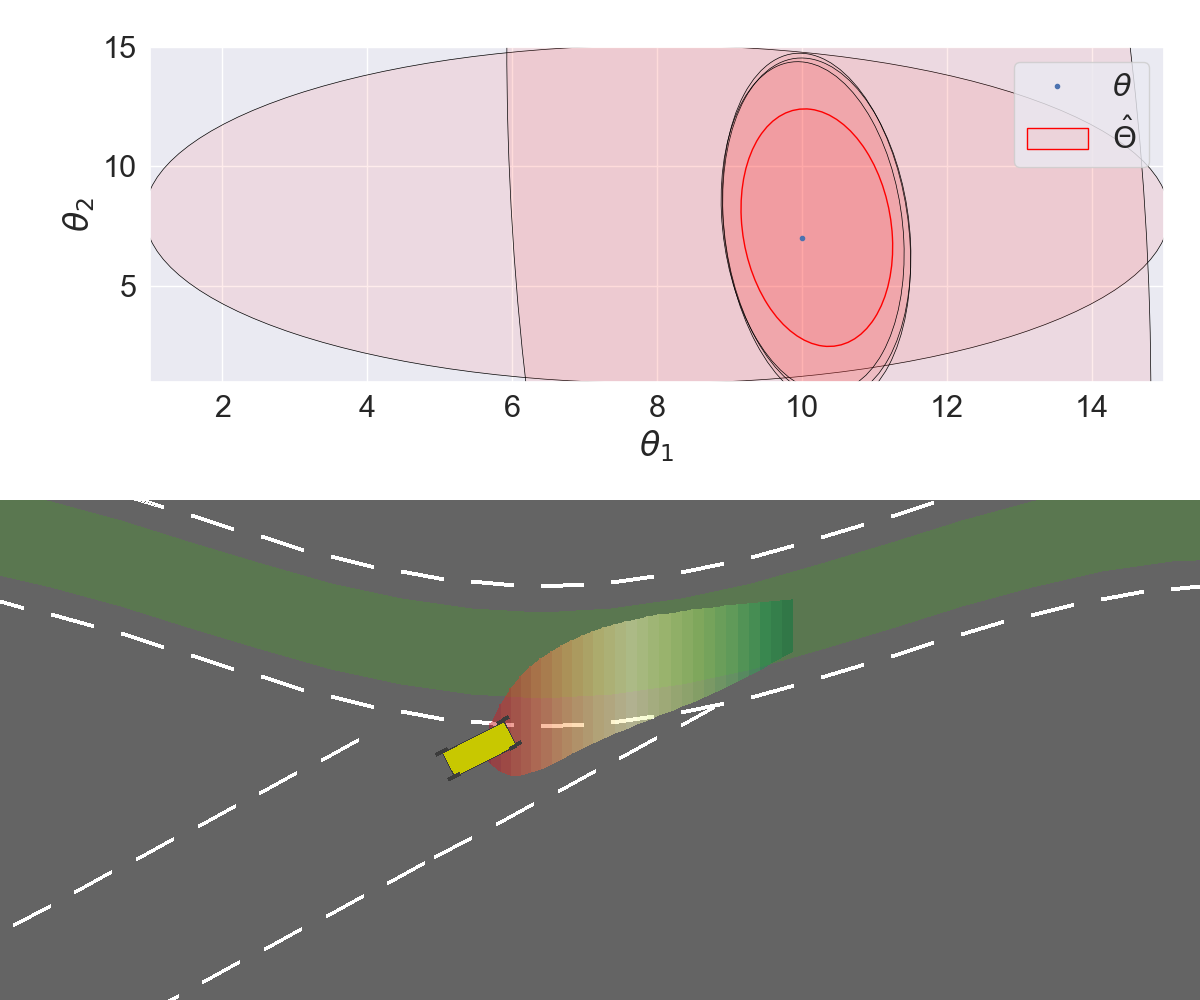
\includegraphics[width=0.9\linewidth]{img/lane-keeping.png}
	\caption{\textbf{Top}: the model estimation showing the confidence region $\hat{\Theta}(t)$ from \eqref{eq:predictor} at different times $t$. \textbf{Bottom}: a lane keeping application, where a car must follow a lane-center curve under unknown friction and perturbations. $X_f$ is shown in green, and $\xi(t)$ as an area with a color gradient.}
	\label{fig:lane-keeping}
\end{figure}

The \Cref{fig:lane-keeping} depicts our approach. The confidence region $\hat{\Theta}(t)$ from \eqref{eq:set_LS} is shown in the top graph, and shrinks with time. To simplify verification of \Cref{assu:metzler} for this example, an auxiliary preliminary feedback has been applied shifting the eigenvalues of the closed-loop system. The robust stability of this feedback is assessed with the LMI of \Cref{thm:ISS_pr}, and we compute the corresponding basin of attraction $X_f$ from \eqref{eq:X_f}, represented in green in the bottom subfigure. Then, we use a sampling-based MPC scheme \cite{HomemDeMello2014} to solve \eqref{eq:LS} and bring $\xi(t)$ into $X_f$ in $T=3s$.  The associated interval prediction $\xi(t)$ from \eqref{eq:predictor} is represented with a color gradient from $t=t_i$ (red) to $t=t_i+T$ (green). Once the vehicles enters $X_f$, we finally switch to the closed-loop feedback \eqref{eq:control_pr} following \eqref{eq:control} for the rest of the simulation. A video is available at this url: \url{https://drive.google.com/file/d/18I6lPgAjS8buMB09OCF6WcHtHzUr_ql_/}.


\section{Minimax control with generic costs}


\label{sec:control}
In order to evaluate the robust objective $V^r$ \eqref{eq:robust-control}, we approximate it thanks to the interval prediction $[\underline{x}(t), \overline{x}(t)]$ of \autoref{sec:prediction}.

\begin{definition}[Surrogate objective]
	\begin{leftbar}[defnbar]
	Let
	\begin{align}
	\label{eq:surrogate_objective} 
	\hat{V}^r(\bu) &\eqdef \sum_{n=N+1}^\infty \gamma^n \underline{R}_n(\bu)\\ 
	\text{where}\quad\underline{R}_n(\bu) &\eqdef \min_{x\in[\underline{x}_n(\bu), \overline{x}_n(\bu)]}  R(x) \label{eq:pessimistic-rewards}
	\end{align}
	and $\underline{x}_n(\bu), \overline{x}_n(\bu)$ follow the dynamics defined in \eqref{eq:interval-predictor}.
	\end{leftbar}
\end{definition}

This amounts to changing the reward function, except that the worst case is assessed over the whole past trajectory, which makes this pessimistic reward $\underline{R_n}$ \emph{not markovian}.

\begin{proposition}[Lower bound]
	\label{prop:lower-bound}
	\begin{leftbar}[propositionbar]
	The surrogate objective  \eqref{eq:surrogate_objective} is a lower bound of the true objective  \eqref{eq:robust-control-disc}: 
	\begin{equation*}
	\hat{V}^r(\bu) \leq V^r(\bu)
	\end{equation*}
	\end{leftbar}
\end{proposition}
A direct consequence is that since all our approximations are conservative, if we manage to find a control sequence such that no \textit{``bad event''} (e.g. a collision) happens according to the surrogate objective $\hat{V}^r$, then we are guaranteed that they will not happen either when the controls are executed on the true system. 

\paragraph{Planning}
To optimise $\hat{V}^r$ \eqref{eq:surrogate_objective}, we cannot use Dynamic Programming algorithms since the state space is continuous and the pessimistic rewards are non-markovian. Instead, we turn to tree-based planning algorithms, which optimise a sequence of actions based on the corresponding sequence of rewards, without requiring markovity nor state enumeration. In particular, we consider the \emph{Optimistic Planning of Deterministic Systems} (\texttt{OPD}) algorithm \citep{Hren2008} tailored for the case when the relationship between actions and rewards is deterministic. Indeed, the stochasticity of the perturbations and measurements is encased in $\hat{V}^r$: given the observations up to time $N$ both the predictor dynamics \eqref{eq:interval-predictor} and the pessimistic rewards \eqref{eq:pessimistic-rewards} are deterministic.

At each planning iteration $k\in[K]$, \texttt{OPD} progressively builds a tree $\cT_{k+1}$ by forming upper-bounds $B_a(k)$ over the value of sequences of actions $a$, and expanding\footnote{The expansion of a leaf node $a$ refers to the simulation of its children transitions $aA = \{ab, b\in A\}$} the leaf $a_k$ with highest upper-bound:
\begin{equation}
\label{eq:opd}
a_k = \argmax_{a\in\cL_k} B_a(k), \quad B_a(k) = \sum_{n=0}^{h(a)-1} \underline{R}_n(a) + \frac{\gamma^{h(a)}}{1-\gamma}
\end{equation}
where $\cL_k$ is the set of leaves of $\cT_k$, $h(a)$ is the length of the sequence $a$, and $\underline{R}_n(a)$ the pessimistic reward \eqref{eq:pessimistic-rewards} obtained at time $n$ by following the controls $u_n = \pi_{a_n}(x_n)$.

\begin{theorem}[Planning performance of \citealt{Hren2008}]
	\label{theorem:opd-regret}
	\begin{leftbar}[theorembar]
	The simple regret of the \texttt{OPD} algorithm \eqref{eq:opd} applied to the surrogate objective \eqref{eq:surrogate_objective} after $K$ planning iterations is
	\begin{align*}
	\text{if } \kappa>1,\quad& 
	\hat{V}^r(a^{\star}) - \hat{V}^r({a_K}) = \cO\left(K^{-\frac{\log 1/\gamma}{\log \kappa}}\right);\\
	\text{if }\kappa=1,\quad&
	\hat{V}^r(a^{\star}) - \hat{V}^r({a_K}) = \cO\left(\gamma^{{(1-\gamma)^{\log_\gamma (\kappa/|\cA|)}}K/{c}}\right)
	\end{align*}
	where $\kappa$ is a problem-dependent measure of the proportion of near-optimal paths:
	\[
	\kappa = \limsup_{h\rightarrow\infty} \left|\left\{a\in A^h: \hat{V}^r(a)\geq \hat{V}^r(a^{\star}) - \frac{\gamma^{h+1}}{1-\gamma}\right\}\right|^{1/h}.
	\]
	\end{leftbar}
\end{theorem}

Hence, by using enough computational budget $K$ for planning we can get as close as we want to the optimal surrogate value $\hat{V}^r(a^{\star})$, at a polynomial rate. Unfortunately, there exists a gap between $\hat{V}^r$ and the true robust objective $V^r$, which stems from three approximations: (i) the true reachable set was approximated by an enclosing interval in \eqref{eq:inclusion-property}; (ii) the time-invariance of the dynamics uncertainty $A(\theta)\in\cC_{[N],\delta}$ was handled by the interval predictor \eqref{eq:interval-predictor} as if it were a time-varying uncertainty $A(\theta(t))\in\cC_{[N],\delta},\forall t$ ; and (iii) the lower-bound $\sum\min\leq \min\sum$ used to define the surrogate objective \eqref{eq:surrogate_objective} is not tight. However, this gap can be bounded with additional assumptions.

\begin{theorem}[Regret bound]
	\label{thm:control-error}
	\begin{leftbar}[theorembar]
	Under three conditions:
	\begin{enumerate}
		\item a Lipschitz regularity assumption for the reward $R$;
		\item a persistent excitation (PE) assumption:
		\begin{align*}
		\exists \underline{\phi},\overline{\phi}>0: \forall n\geq n_0,\quad \underline{\phi}^2 \leq \lambda_{\min}(\Phi_{n}^\transp\Sigma_{p}^{-1}\Phi_{n}) \leq \overline{\phi}^2;
		\end{align*}
		\item a stability condition: there exist $P>0,Q_0\in\Real^{p\times p}$, $\rho>0$ such that
		$\begin{bmatrix}
		A_0^\transp P + P A_0^\transp + Q_0 & P|D|  \\
		|D|^\transp P & -\rho I_r \\
		\end{bmatrix}< 0;$
	\end{enumerate}
	we can bound the approximation error of \autoref{alg:full}:
	\begin{equation*}
	\hat{V}^r(\bu) \leq {V}^r(\bu) \leq V(\bu) \leq \hat{V}^r(\bu) + \Delta_\omega + \cO\left({\log N / N}\right)
	\end{equation*}
	with probability at least $1-\delta$, where $\Delta_\omega$ is a constant which corresponds to an irreducible suboptimality suffered from being robust to instantaneous perturbations $\omega(t)$.
	\end{leftbar}
\end{theorem}


\section{Multi-model selection}
\label{sec:multi-model}

The procedure we developed in sections \ref{sec:estimation}, \ref{sec:prediction} and \ref{sec:control} relies on strong modelling assumptions, such as the linear dynamics \eqref{eq:dynamics} and \autoref{assumpt:structure}. But what if they are wrong?

\paragraph{Model adequacy}

One of the major benefits of using the family of linear models, compared to richer model classes, is that they provide strict conditions allowing to quantify the adequacy of the modelling assumptions to the observations.

Given $N-1$ observations, \autoref{sec:estimation} provides a polytopic confidence region \eqref{eq:polytope} that contains $A(\theta)$ with probability at least $1-\delta$. Since the dynamics are linear, we can propagate this confidence region to the next observation: $y_{N}$ must belong to the Minkowski sum of a polytope representing model uncertainty $\cP(A_{0} x_N + Bu_N, \Delta A_{1}x_N,\dots, \Delta A_{2^d}x_N)$ and a polytope $\cP(0_p, \underline{\eta}, \overline{\eta})$ bounding the perturbation and measurement noises. \citet{delos2015} provide a way to test this membership in polynomial time using linear programming. Whenever it is not verified, we can confidently reject the $(A,\phi)$-modelling \autoref{assumpt:structure}. This enables us to consider a rich set of potential features $\left((A^1, \phi^1), \dots, (A^M, \phi^M)\right)$ rather than relying on a single assumption, and only retain those that are consistent with the observations so far. Then, every remaining hypothesis must be considered during planning.

\paragraph{Robust selection}

We temporarily ignore the parametric uncertainty on $\theta$ to simply consider several candidate dynamics models, which all correspond to different modelling assumptions. We also restrict to deterministic dynamics, which is the case of \eqref{eq:interval-predictor}.

\begin{assumption}[Multi-model ambiguity]
	\label{assumpt:multi-model-ambiguity}
	\begin{leftbar}[assumptionbar]
	The true dynamics $f$ lies within a finite set of candidate models $f^1, \dots, f^M$.
	\begin{equation*}
	\exists m\in[M]: \dot{x}(t) = f^m(x(t), u(t)), \forall t\geq 0
	\end{equation*}
	\end{leftbar}
\end{assumption}
We want to adapt our planning algorithm in order to balance these concurrent hypotheses in a robust fashion, i.e. maximise a robust objective with discrete ambiguity
\begin{equation}
\label{eq:robust-objective-discrete}
V^r = \sup_{a\in\cA^\Natural}\min_{m\in[M]} \sum_{n=N+1}^\infty \gamma^n R_n^m
\end{equation}
where $R_n^m$ is the reward obtain by following the action sequence $a$ up to step $n$ under the dynamics $f^m$.
This objective could be optimised in the same way as in \autoref{sec:control}, but this would result in a coarse and lossy approximation. Instead, we exploit the finite uncertainty structure of \autoref{assumpt:multi-model-ambiguity} to asymptotically recover the true $V^r$ by modifying the \texttt{OPD} algorithm in the following way:

\begin{definition}[Robust sequence upper bounds]
	\begin{leftbar}[defnbar]
	We replace the upper-bound \eqref{eq:opd} on sequence values in \texttt{OPD} by
	\begin{equation}
	\label{eq:robust-b-values}
	B_a^r(k)  \eqdef \min_{m\in[M]} \sum_{n=0}^{h-1} \gamma^n R_n^m  + \frac{\gamma^h}{1-\gamma}
	\end{equation}
	\end{leftbar}
\end{definition}
An illustration of the computation of the robust upper-bounds is presented in Figure \ref{fig:drop}. 
Note that it is not equivalent to solving each control problem independently and following the action with highest worst-case value:
\begin{remark}
	\label{sec:min-max-order}
	\begin{leftbar}[remarkbar]
	In the definition of $B_{a}^{r}(k)$ \eqref{eq:br} and $U_{a}^{r}(k)$ \eqref{eq:ur} it is essential that the minimum over the models is only taken at the end of trajectories, in the same way as for the robust objective \eqref{eq:robust-objective-discrete} in which the worst-case dynamics is only determined after the action sequence has been fully specified. Assume that $U_{a}^{r}(k)$ is instead naively defined as
	
	\[
	U_{a}^{r}(k)=\min_{m\in[1,M]}U_{a}^{m}(k),
	\]
	
	This would not recover the robust policy, as we show in \autoref{fig:min-max-order} with a simple counter-example.
\end{leftbar}
	\begin{figure}[htp]
	\centering
	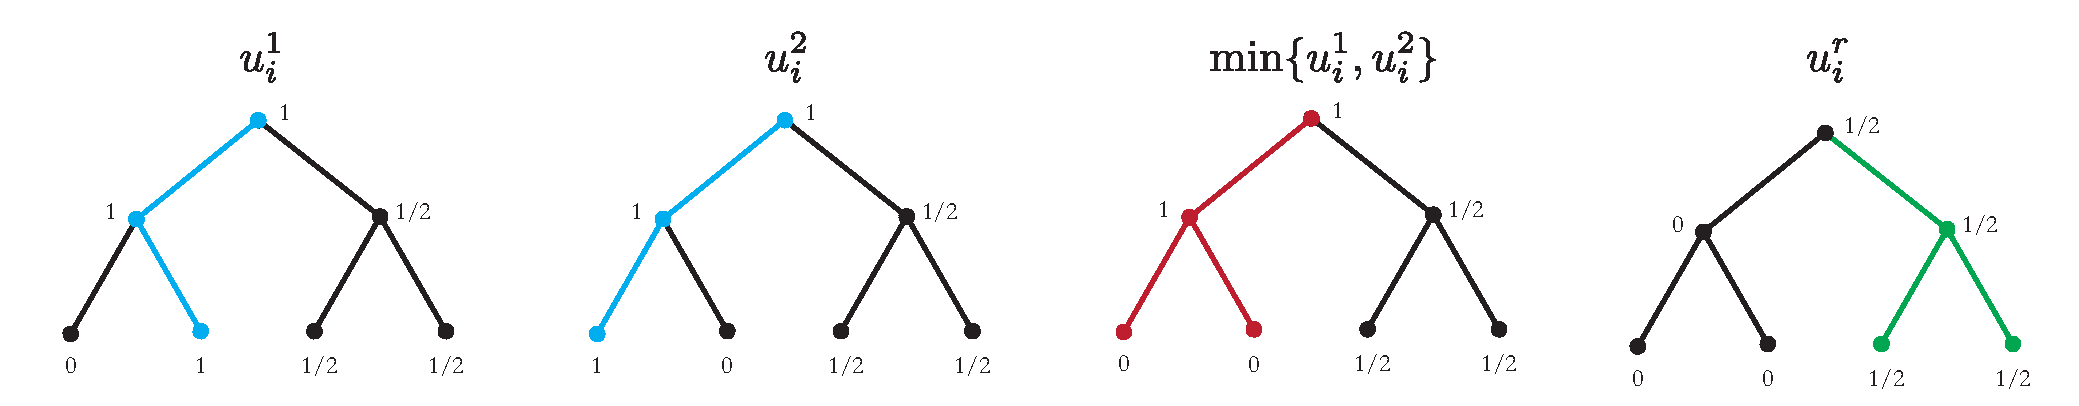
\includegraphics[width=\linewidth]{img/min-max-order}
	\caption{From left to right: two simple models and corresponding u-values with optimal sequences in blue; the naive version of the robust values returns sub-optimal paths in red; our robust U-value properly recovers the robust policy in green.}
	\label{fig:min-max-order}
	\end{figure}
\end{remark}

We analyse the sample complexity of the corresponding robust planning algorithm.

\begin{figure}
	\centering
	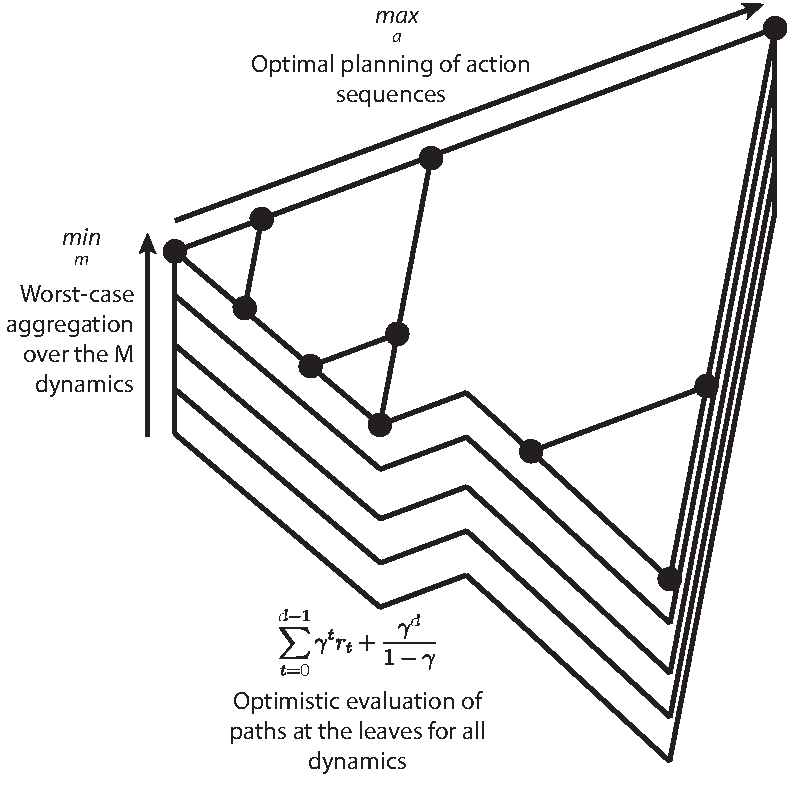
\includegraphics[width=0.45\linewidth]{img/robust-control-tree}
	\caption{The computation of robust B-values in \eqref{eq:robust-b-values}. The simulation of trajectories for every dynamics model $f^m$ is represented as stacked versions of the expanded tree $\mathcal{T}_k$.}
	\label{fig:drop}
\end{figure}

\begin{theorem}[Robust planning performance]
	\label{theorem:drop-regret}
	\begin{leftbar}[theorembar]
	The robust version of \texttt{OPD} \eqref{eq:robust-b-values} enjoys the same regret bound as \texttt{OPD} in \autoref{theorem:opd-regret}, with respect to the multi-model objective \eqref{eq:robust-objective-discrete}.
	\end{leftbar}
\end{theorem}

The regret depends on the number $K$ of node expansions, but each expansion now requires $M$ times more simulations than in the single-model setting. The solution of the robust objective \eqref{eq:robust-objective-discrete} with discrete ambiguity $f\in\{f^m\}_{m\in[M]}$ can be recovered exactly, asymptotically when the planning budget $K$ goes to infinity. This contrasts the results obtained in \autoref{sec:control} for the robust objective \eqref{eq:robust-control} with continuous ambiguity $A(\theta)\in\cC_{[N],\delta}$, for which \texttt{OPD} only recovers the surrogate approximation $\hat{V}^r$, as discussed in \autoref{thm:control-error}. Finally, the two approaches of Sections \ref{sec:control} and \ref{sec:multi-model} can be merged by using the pessimistic reward \eqref{eq:pessimistic-rewards} in \eqref{eq:robust-b-values}.

\section{Experiments}
\label{sec:interval-experiments}

\paragraph{Obstacle avoidance with unknown friction}
We first consider a simple illustrative example, shown in \autoref{fig:prediction}: the control of a 2D system with position $(p_x,p_y)$ and velocity $(v_x, v_y)$ moving by means of a force $(u_x, u_y)$ in an environment with unknown anisotropic friction.

\begin{equation*}
\begin{bmatrix}
\dot{p_x}\\
\dot{p_y}\\
\dot{v_x}\\
\dot{v_y}\\
\end{bmatrix} = 
\begin{bmatrix}
0 & 0 & 1 & 0 \\
0 & 0 & 0 & 1 \\
0 & 0 & -\theta_x & 0 \\
0 & 0 & 0 & -\theta_y
\end{bmatrix}
\begin{bmatrix}
{p_x}\\
{p_y}\\
{v_x}\\
{v_y}\\
\end{bmatrix}
+
\begin{bmatrix}
0\\
0\\
{u_x}\\
{u_y}\\
\end{bmatrix}
\end{equation*}


% TODO: \autoref{assumpt:metzler}
Note that the Metzler assumption for $A_0$ is always verified. The reward is non-smooth and encodes the task of navigating to reach a goal state $x_g$ while avoiding collisions with obstacles: $R(x) = \delta(x)/(1 + \|x - x_g\|_2)$  where $\delta(x)$ is $0$ whenever $x$ collides with an obstacle, $1$ otherwise. The actions $\cA$ are constant controls in the up, down, left and right directions.

We run \autoref{alg:full} for 100 simulations, and compare in \autoref{tab:obstacle} its performances to that of the nominal agent, i.e. the non-robust adaptive control approach that plans with the estimated dynamics $\theta_{[N],\lambda}$. We observe that though the robust agent performs worse than the nominal agent on average, it manages to ensure safety and attains a better worst-case performance, as intended. We also study the evolution of the simple regret $V(x_n) - J_n(x_n)$ with respect to the number of samples $N$, where $J_n(x_n) = \sum_{i > n} \gamma^i R_i$ is the empirical return at state $x_n$ in a trajectory $x_0, R_0, x_1, R_1, \dots$, while $V(x_n)$ is the optimal value that the agent would get by acting optimally from $x_n$ with knowledge of the dynamics. The mean regret is shown in \autoref{fig:regret}, along with its 95\% confidence interval. We see that \autoref{alg:full} has a regret $\hat{V}^r - V$ decreasing at least polynomially with $N$, as expected from \autoref{thm:control-error}. This shows that the agent gets more aggressive when it is more confident, as desired, while ensuring safety at all time. In contrast, the nominal agent has an even smaller regret but collided with obstacles in $4\%$ of simulations.

\begin{figure}[tp]
	\centering
	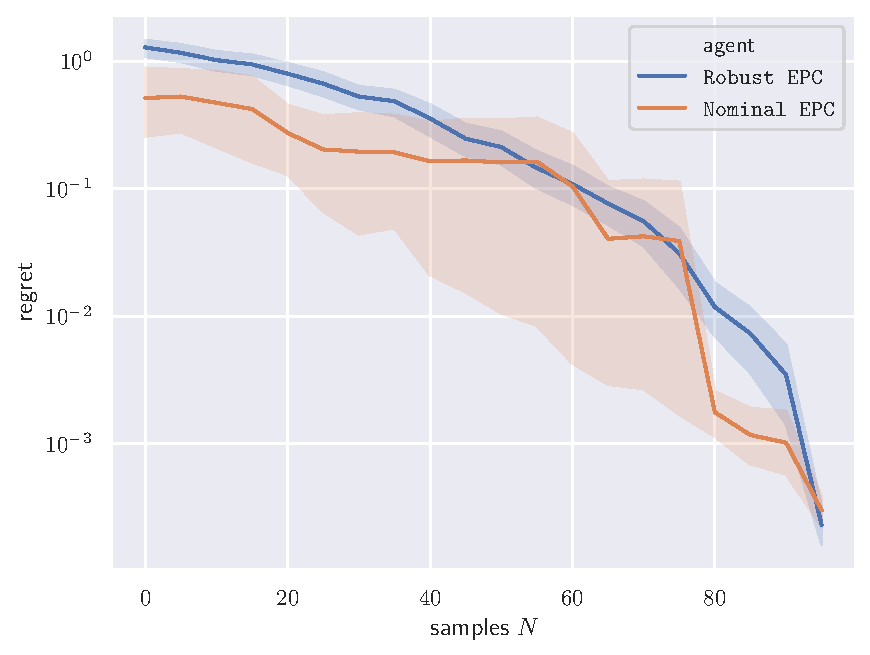
\includegraphics[width=0.8\linewidth]{img/regret.pdf}
	\caption{The mean regret along with its $95\%$ confidence interval with respect to $N$, for the robust and nominal agents.}
	\label{fig:regret}
\end{figure}

\begin{table}[tbp]
	\caption{Performances on the obstacle avoidance task}
	\label{tab:obstacle}
	\centering
	\begin{tabular}{lccc}
		\toprule
		Agent &
		failures &
		min return &
		mean return $\pm$ std  \\
		\midrule
		Oracle & 0\% & {11.6} & {$14.2 \pm 1.3$} \\
		\midrule
		{Nominal} & {4\%} & {2.8} & \textbf{$\mathbf{13.8} \pm 2.0$} \\
		\autoref{alg:full} & \textbf{0\%} & \textbf{10.4} & {$13.0 \pm 1.5$} \\
		\bottomrule
	\end{tabular}
\end{table}

\paragraph{Behavioural planning for an autonomous vehicle}
We consider the \href{https://github.com/eleurent/highway-env}{highway-env} environment \citep{highway-env} for simulated driving decision problems. An autonomous vehicle with state $\chi_0\in\Real^4$ is approaching an intersection among $V$ other vehicles with states $\chi_i\in\Real^4$, resulting in a joint traffic state $x = [\chi_0, \dots,\chi_V]^\top\in\Real^{4V+4}$. These vehicles follow parametrized behaviours $\dot{\chi}_i=f_i(x,\theta_i)$ with unknown parameters $\theta_i\in\Real^5$. We appreciate a first advantage of the structure imposed in \autoref{assumpt:structure}: the uncertainty space of $\theta$ is $\Real^{5V}$. In comparison, the traditional LQ setting where the whole state matrix $A$ is estimated would have resulted in a much larger parameter space $\theta\in\Real^{16V^2}$.
%This allows to scale to larger systems: in our experiments, we used a state space of dimension $44$ ($V=10$) where e.g. \citep{Dean2018,abeille18a} reported numerical experiments with states of dimensions 3 and 4, respectively.
The system dynamics $f$, which describes the couplings and interactions between vehicles, can only be expressed in the form of \autoref{assumpt:structure} given the knowledge of the desired route for each vehicle, with features $\phi$ expressing deviations to the centerline of the followed lane. Since these intentions are unknown to the agent, we adopt the multi-model perspective of \autoref{sec:multi-model} and consider one model per possible route for every observed vehicle before an intersection. We compare \autoref{alg:full} to a nominal agent planning with the estimated parameter $\theta_{[N],\lambda}$, with two different modelling assumptions: we assume that Nominal 1 has access to the true followed route for each vehicle, while Nominal 2 does not and picks a model with minimal prediction error. Their performances are compared in \autoref{tab:driving}. Again, the robust approach is less efficient on average than planning with a nominal model, but it does better in terms of worst-case performance and manages to avoid collisions, contrary to the nominal baselines that suffer from model bias. We provide more details about the system and videos of the experiments in the Supplementary Material.

\begin{figure}[t]
	\centering
	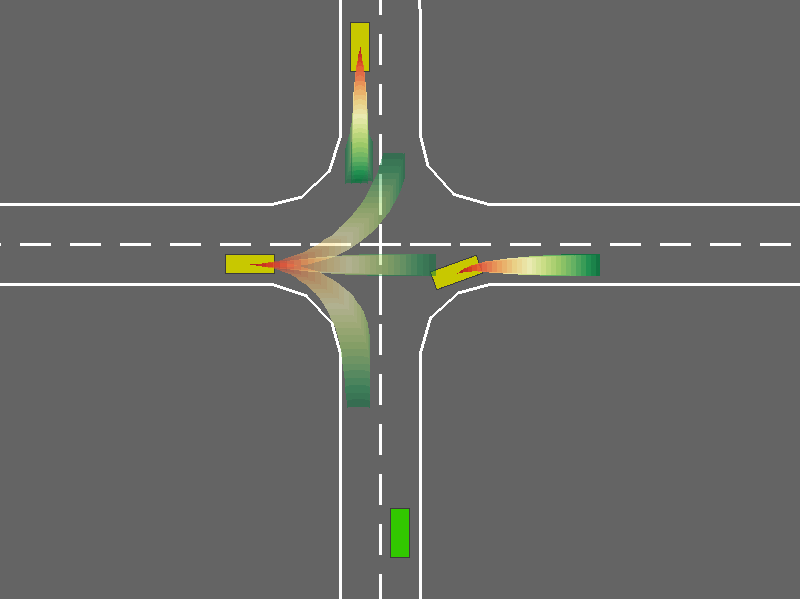
\includegraphics[width=0.7\linewidth]{img/highway-small}
	\caption{The intersection crossing task. We show the trajectory intervals corresponding to behavioural uncertainty for each observed vehicle, and the multi-model assumption over the followed route.}
\end{figure}

\begin{table}[t]
	\caption{Performances on the driving task}
	\label{tab:driving}
	\centering
	\begin{tabular}{lccc}
		\toprule
		Agent &
		failures &
		min return &
		mean return $\pm$ std  \\
		\midrule
		Oracle & 0\% & {6.9} & $7.4 \pm 0.5$ \\
		\midrule
		{Nominal 1} & 4\% & {5.2} & $\mathbf{7.3} \pm 1.5$ \\
		{Nominal 2} & 33\% & {3.5} & $6.4 \pm 0.26$ \\
		\autoref{alg:full} & \textbf{0\%} & \textbf{6.8} & $7.1 \pm 0.29$ \\
		\bottomrule
	\end{tabular}
\end{table}

\section*{Conclusion}

We present a framework for the robust estimation, prediction and control of a partially known linear system with generic costs. Leveraging tools from linear regression, interval prediction, and tree-based planning, we guarantee the predicted performance and provide a regret bound. The applicability of the method is further improved by a multi-model extension and demonstrated on two simulated applications.

\begin{subappendices}
	
	\section{Proofs}
	\label{sec:proof}
	
	\subsection{Proof of \autoref{prop:regularized_solution}}
	
	\begin{proof}
		We differentiate $J(\theta) = \sum_{n=1}^N \|y_n -\Phi_n\theta\|_{\Sigma_p^{-1}}^2 + \lambda\|\theta\|_{}^2$ as in  \eqref{eq:regression_min} with respect to $\theta$:
		
		\begin{align*}
		\nabla_{\theta} J(\theta) &= \sum_{n=1}^N\nabla_{\theta} (y_n - \Phi_n\theta)^\transp\Sigma_p^{-1}(y_n - \Phi_n\theta) + \nabla_{\theta} \lambda\|\theta\|_{}^2\\
		&= -2\sum_{n=1}^N y_n^\transp\Sigma_p^{-1}\Phi_n + 2\sum_{n=1}^N\theta^\transp(\Phi_n^\transp\Sigma^{-1}\Phi_n) +  2 \lambda \theta^\transp
		\end{align*}
		
		Hence,
		\begin{align*}
		\nabla_{\theta} J(\theta) = 0 \iff \left(\sum_{n=1}^N\Phi_n^\transp\Sigma_p^{-1}\Phi_n + I_d\right)\theta = \sum_{n=1}^N y_n^\transp\Sigma_p^{-1}\Phi_n
		\end{align*}
	\end{proof}
	
	\subsection{Proof of \autoref{thm:confidence_ellipsoid}}
	
	We start by showing a preliminary proposition:
	
	\begin{proposition}[Matrix version of Theorem 1 of \citealt{Abbasi2011}]
		\label{prop:concentration}
		\begin{leftbar}[propositionbar]
		Let $\{F_n\}_{n=0}$ be a filtration.
		Let $\{\eta_n\}_{n=1}^\infty$ be a $\Real^p$-valued stochastic process such that $\eta_n$ is $F_n$-measurable and $\expectedvalue\left[\eta_n\condbar F_{n-1}\right]$ is $\Sigma_p$-sub-Gaussian.
		
		Let $\{\Phi_n\}_{n=1}^\infty$ be an $\Real^{p\times d}$-valued stochastic process such that $\Phi_n$ is $F_n$-measurable. Assume that $G$ is a $d\times d$ positive definite matrix. For any $n\geq 0$, define
		\begin{equation*}
		\overline{G}_n = G + \sum_{s=1}^n \Phi_s^\transp \Sigma_p^{-1} \Phi_s \in \Real^{d\times d} \quad S_n = \sum_{s=1}^n \Phi_s^\transp\Sigma_p^{-1}\eta_s \in \Real^{d}.
		\end{equation*}
		Then, for any $\delta>0$, with probability at least $1-\delta$, for all $n\geq0$,
		\begin{align*}
		\| S_n \|_{\overline{G}_n^{-1}} \leq \sqrt{2\ln \left(\frac{\det\left(\overline{G}_n\right)^{1/2}}{\delta\det(G)^{1/2}}\right)}.
		\end{align*}
		\end{leftbar}
	\end{proposition}
	\begin{proof}
		Let 
		\begin{equation*}
		G_t = \sum_{s=1}^t \Phi_s^\transp \Sigma_p^{-1} \Phi_s \in \Real^{d\times d}
		\end{equation*}
		And for any $z\in\Real^d$,
		\begin{equation*}
		M_t^z = \exp{\left(\inp{z}{S_t} - \frac{1}{2}\|z\|_{G_t}\right)}
		\end{equation*}
		\begin{equation*}
		D_t^z = \exp{\left(\inp{\Phi_t z}{\eta_t}_{\Sigma_p^{-1}} - \frac{1}{2}\|\Phi_t z\|_{\Sigma_p^{-1}}\right)}
		\end{equation*}
		Then,
		\begin{align*}
		M_t^z &= \exp{\left(\sum_{s=1}^t z^\transp \Phi_s^\transp \Sigma_p^{-1} \eta_s - \frac{1}{2} (\Phi_s z)^\transp\Sigma_p^{-1}(\Phi_s z) \right)} \\
		&= \prod_{s=1}^{t} D_s^z
		\end{align*}
		and using the Sub-Gaussianity of $\eta_t$
		\begin{align*}
		\expectedvalue\left[D_t^z \condbar F_{t-1}\right] = {}& \exp{\left(- \frac{1}{2}\|\Phi_t z\|_{\Sigma_p^{-1}}\right)}\\ &\expectedvalue\left[\exp{\left(\inp{\Phi_t z}{\eta_t}_{\Sigma_p^{-1}}\right)} \condbar F_{t-1}\right]  \\
		\leq {} & \exp{\left(- \frac{1}{2}\|\Phi_t z\|_{\Sigma_p^{-1}}\right)}\\
		&\exp{\left((z^\transp \Phi_t^\transp \Sigma_p^{-1})\Sigma_p(\Sigma_p^{-1} \Phi_t z)\right)}\\
		&= 1
		\end{align*}
		\begin{align*}
		\expectedvalue\left[M_t^z \condbar F_{t-1}\right] = \left(\prod_{s=1}^{t-1} D_s^z\right) \expectedvalue\left[D_t^z \condbar F_{t-1}\right] \leq M_{t-1}^z
		\end{align*}
		Showing that $(M_t^z)_{t=1}^\infty$ is indeed a supermartingale and in fact $\expectedvalue[M_t^z]\leq 1$.
		It then follows by Doob's upcrossing lemma for supermartingale that $M_\infty^z = \lim_{t\to\infty} M_t^z$ is almost surely well-defined, and so is $M_\tau^z$ for any random stopping time $\tau$.
		
		Next, we consider the stopped martingale $M_{\min(\tau,t)}^z$. Since 
		$(M_t^z)_{t=1}^\infty$ is a non-negative supermartingale and $\tau$ is a random stopping time, we deduce by Doob's decomposition that
		\begin{align*}
		\expectedvalue[M_{\min(\tau,t)}^z] &= \expectedvalue[M_0^z] + \expectedvalue[\sum_{s=0}^{t-1} (M_{s+1}^z-M_s^z) \mathbb{I}\{\tau>s\}]\\
		&\leq 1 + \expectedvalue[\sum_{s=0}^{t-1} \expectedvalue[M_{s+1}^z-M_s^z|F_{s}] \mathbb{I}\{\tau>s\}]\\
		&\leq 1
		\end{align*}
		Finally, an application of Fatou's lemma show that 
		$\expectedvalue[M_\tau^z] = \expectedvalue[\liminf_{t\to\infty} M_{\min(\tau,t)}^z] \leq \liminf_{t\to\infty} \expectedvalue[M_{\min(\tau,t)}^z] \leq 1.$
		
		This results allows to apply a result from \citep{pena2008self}.
		\begin{lemma}[Theorem 14.7 of \citep{pena2008self}]
			\begin{leftbar}[lemmabar]
			If $Z$ is a random vector and $B$ is a symmetric positive definite matrix such that
			\[\forall \gamma\in\Real^d, \ln \expectedvalue \exp \left(\gamma^\transp Z -\frac{1}{2} \gamma^\transp B \gamma \right)\leq 0,\]
			then for any positive definite non-random matrix C, it holds
			\[\expectedvalue\left[ \sqrt{\frac{\det(C)}{\det(B+C)} } \exp\left( \frac{1}{2}\|Z\|^2_{(B+C)^{-1}}\right)\right]\leq 1. \] 
			In particular, by Markov inequality, for all $\delta\in(0,1)$, 
			\[\probability{\|Z\|_{(B+C)^{-1}} \geq \sqrt{2\ln \left(\frac{\det \left((B+C)^{1/2}\right)}{\delta\det(C)^{1/2}}\right)}}\leq \delta.\]
			\end{leftbar}
		\end{lemma}
		
		Here, by using $Z = \sum_{s=1}^t\Phi_s\Sigma_p^{-1}\eta_s$, $B=G_t$, $C=G$,
		
		\[
		\probability{\| S_t \|_{(G_t+G)^{-1}} \geq \sqrt{2\ln \left(\frac{\det(G_t+G)^{1/2}}{\delta\det(G)^{1/2}}\right)}} \leq \delta
		\]
		
	\end{proof}
	
	Having shown this preliminary result, we move on to the proof of \autoref{thm:confidence_ellipsoid}.
	
	\begin{proof}
		For all $x\in\Real^d$, \eqref{eq:vector_rls} gives
		\begin{align*}
		x^\transp\theta_{N,\lambda}  -x^\transp\theta &= x^\transp G_{N, \lambda}^{-1}\sum_{n=1}^N \Phi_n^\transp \Sigma_p^{-1}\eta_n
		- \lambda x^\transp G_{N, \lambda}^{-1}\theta\\
		&= \inp{x}{\sum_{n=1}^N \Phi_n^\transp \Sigma_p^{-1}\eta_n}_{G_{N, \lambda}^{-1}} - \lambda\inp{x}{\theta}_{G_{N, \lambda}^{-1}}
		\end{align*}
		
		Using the Cauchy-Schwartz inequality, we get
		\begin{align*}
		|x^\transp\theta_{N,\lambda}  -x^\transp\theta| \leq {} & \|x\|_{G_{N, \lambda}^{-1}}\left(\left\|\sum_{n=1}^N \Phi_n^\transp \Sigma_p^{-1}\eta_n\right\|_{G_{N, \lambda}^{-1}}\right.\\ 
		&+ \left.\lambda\|\theta\|_{G_{N, \lambda}^{-1}}\right)
		\end{align*}
		
		In particular, for $x = G_{N,\lambda}(\theta_{N,\lambda} - \theta)$, we get after simplifying with $\| \theta_{N,\lambda}  - \theta\|_{G_{N,\lambda}}$,
		\begin{align*}
		\| \theta_{N,\lambda}  - \theta\|_{G_{N,\lambda}} &\leq \left\|\sum_{n=1}^N \Phi_n^\transp \Sigma_p^{-1}\eta_n\right\|_{G_{N, \lambda}^{-1}} + \lambda\|\theta\|_{G_{N, \lambda}^{-1}}
		\end{align*}
		
		By applying \autoref{prop:concentration} with $G=\lambda I_d$, we obtain that with probability at least $1-\delta$,
		\begin{align*}
		\| \theta_{N,\lambda}  - \theta\|_{G_{N,\lambda}} &\leq \sqrt{2\ln \left(\frac{\det(G_{N,\lambda})^{1/2}}{\delta\det(\lambda I_d)^{1/2}}\right)}
		+ \lambda\|\theta\|_{G_{N, \lambda}^{-1}}
		\end{align*}
		And since $\|\theta\|_{G_{N, \lambda}^{-1}}^2 \leq 1/\lambda_{\min}(G_{N,\lambda})\|\theta\|_2^2 \leq 1/\lambda \|\theta\|_2^2$ and $\|\theta\|_2^2 \leq d\|\theta\|_\infty^2\leq d S^2$,
		\begin{align*}
		\| \theta_{N,\lambda}  - \theta\|_{G_{N,\lambda}} &\leq \sqrt{2\ln \left(\frac{\det(G_{N,\lambda})^{1/2}}{\delta\det(\lambda I_d)^{1/2}}\right)}
		+ (\lambda d)^{1/2}S
		\end{align*}
	\end{proof}
	
	
	\subsection{Proof of \autoref{prop:lower-bound}}
	
	\begin{proof}
		The predictor designed in \autoref{sec:prediction} verifies the inclusion property \eqref{eq:inclusion-property}. Thus, for sequence of controls $\bu$, any dynamics $A(\theta)\in C_{[N],\delta}$, and perturbations $\underline{\bom} \leq \bom \leq \overline{\bom}$, the corresponding state at time $t_n$ is bounded by $\underline{x}_n \leq x_n \leq \overline{x}_n$, which implies that $R(x_n) \geq \min_{x\in[\underline{x}_n(\bu), \overline{x}_n(\bu)]}  R(x) = \underline{R}_n(\bu)$.
		
		Thus, by taking the min over $C_{[N],\delta}$ and $[\underline{\bom}, \overline{\bom}]$, we also have for any sequence of controls $\bu$,
		\begin{align*}
		V^r(\bu) &= \min_{\substack{A(\theta)\in C_{[N],\delta}\\ \underline{\bom} \leq \bom \leq \overline{\bom}}} \sum_{n=N+1}^\infty \gamma^n R(x_n)\\
		&\geq \sum_{n=N+1}^\infty \gamma^n \underline{R}_n(\bu)\\
		&= \hat{V}^r(\bu)
		\end{align*}
	\end{proof}
	
	\subsection{Proof of \autoref{thm:control-error}}
	
	We first bound the model estimation error.
	\begin{lemma}
		\begin{leftbar}[lemmabar]
		If the features $\Phi_n$ are persistently exciting:
		\begin{align}
		\label{eq:excitation}
		\exists \underline{\phi},\overline{\phi}>0, n_0: \forall n\geq n_0,\nonumber\\ \underline{\phi}^2 \leq \lambda_{\min}(\Phi_{n}^\transp\Sigma_{p}^{-1}\Phi_{n}) \leq \overline{\phi}^2,
		\end{align}
		then,
		\[\|A(\theta) - A(\theta_{[N],\lambda})\|_2 = \cO\left( \sqrt{\frac{\log N}{N}} \right) \]
	\end{leftbar}
	\end{lemma}
	\begin{proof}
		By \eqref{eq:g_n_lambda} and \eqref{eq:excitation}, we have $$\lambda_{\min}(G_{[N],\lambda,i,j}) \geq (N-n_0)\underline{\phi}^2 + \sum_{n<n_0}\Phi_{n}^\transp\Sigma_{p}^{-1}\Phi_{n}$$
		
		Hence, by \eqref{eq:confidence-ellipsoid} we have 
		\begin{align*}
		\|\theta - \theta_{[N],\lambda}\|_{G_{[N],\lambda}} \geq (\sqrt{N}\underline{\phi} + \cO(1))\|\theta - \theta_{[N],\lambda}\|_{2}
		\end{align*}
		and \eqref{eq:beta_n} gives
		
		\begin{align*}
		\beta_N(\delta) &= \sqrt{2\ln \left(\frac{\det(G_{N,\lambda})^{1/2}}{\delta\det(\lambda I_d)^{1/2}}\right)}
		+ (\lambda d)^{1/2}S\\
		&\leq \sqrt{d\log (N\overline{\phi}^2) / \lambda^{d/2}} + \cO(1)
		\end{align*}
		Thus,
		\[\|\theta - \theta_{[N],\lambda}\|_{2} = \cO\left( \sqrt{\frac{\log N}{N}} \right) \]
		
		And $A(\theta)$ belongs to a linear image of this $L^2$-ball. By writing a the $j^{th}$ column of a matrix $M$ as $M_j$, and its coefficient $i,j$ as $M_{i,j}$,
		\begin{align*}
		((A(\theta)&-A(\theta_{[N],\lambda}))^\transp (A(\theta) - A(\theta_{[N],\lambda})))_{i,j}\\
		%&= (\phi_i(\theta-\theta_{[N],\lambda}))^\transp \phi_j(\theta-\theta_{[N],\lambda}) \\
		&= (\theta-\theta_{[N],\lambda})^\transp\phi_{i}^{\transp}\phi_j(\theta-\theta_{[N],\lambda}) \\
		&\leq \lambda_{\max}(\phi_{i}^{\transp}\phi_j) \|\theta - \theta_{[N],\lambda}\|_{2}^2 = \cO\left( {\frac{\log N}{N}} \right) 
		\end{align*}
		
	\end{proof}
	
	Then, we propagate this estimation error through the state prediction.
	
	\begin{lemma}
		\begin{leftbar}[lemmabar]
		If there exist $P>0,Q_0\in\Real^{p\times p}$, $\rho>0$ such that
		\begin{align*}
		\begin{bmatrix}
		A_0^\transp P + P A_0^\transp + Q_0 & P|D|  \\
		|D|^\transp P & -\rho I_r \\
		\end{bmatrix}< 0,
		\end{align*}
		then for all $t> t_N$,
		\[\|\ox(t) - \ux(t)\| \leq \left(C_0 + \cO\left({\frac{\log N}{N}} \right)\right)C_\omega(t), \]
		where $$C_0 = \sqrt{\frac{2\rho\lambda_{\max}(P)}{\lambda_{\min}(P)\lambda_{\min}(Q_0)}},$$ and $$C_\omega(t) = \sup_{\tau\in[t_N,t]} \|\overline{\omega}(\tau) - \underline{\omega}(\tau)\|_2^2.$$
		\end{leftbar}
	\end{lemma}
	\begin{proof}
		Let $e = \ox - \ux$. \eqref{eq:interval-predictor} gives the dynamics
		\begin{align*}
		\dot{e} = A_0e + |\Delta A|(\ox^+ + \ux^-) + |D|(\overline{\omega} - \underline{\omega})
		\end{align*}
		where recall that $|M| = M^+ + M^-$ for any matrix $M\in\Real^{p\times p}$.
		
		We define the Lyapunov function $V = e^\transp P e$, which is non-negative definite provided that
		$
		P>0,
		$ and compute its derivative
		\begin{align*}
		\dot{V} ={}& X^\transp
		\begin{bmatrix}
		A_0^\transp P + P A_0^\transp + Q & P|D| & P|\Delta A| \\
		|D|^\transp P & -\rho I_r & 0\\
		|\Delta A|^\transp P & 0 & -\alpha I_p
		\end{bmatrix}
		X\\
		& - e^\transp Q e + \alpha |\ux^+ + \ox^-|^2 + \rho |\overline{\omega} - \underline{\omega}|^2
		\end{align*}
		with $X=\begin{bmatrix}
		e & \overline{\omega} - \underline{\omega} &  \ux^+ + \ox^-
		\end{bmatrix}^\transp$, for any $Q\in\Real^{p\times p}$, $\rho,\alpha\in\Real$ . 
		
		Moreover, it holds that $-\ux^+ -\ox^- \leq e \leq \ox^+ + \ux^-$, which implies $|\ux^+ + \ox^-| \leq 2 |e|$. Hence,
		\begin{align*}
		\dot{V} \leq {}& X^\transp
		\underbrace{
			\left[
			\begin{array}{cc|c}
			A_0^\transp P + P A_0^\transp + Q + 4\alpha I_p & P|D| & P|\Delta A| \\
			|D|^\transp P & -\rho I_r & 0\\
			\hline
			|\Delta A|^\transp P & 0 & -\alpha I_p
			\end{array}
			\right]}_{\Upsilon}
		X\\
		& - e^\transp Q e + \rho \|\overline{\omega} - \underline{\omega}\|_2^2
		\end{align*}
		
		Thus, if we had $\Upsilon \leq 0$, $Q>0$, $\rho > 0$, then we would have
		\[
		\dot{V} \leq -\mu V + \rho \|\overline{\omega} - \underline{\omega}\|_2^2
		\]
		with $\mu = \frac{\lambda_{\min}(Q)}{\lambda_{\max}(P)}$. Since $V(t_N) = 0$, this further implies that for all $t>t_N$, 
		\begin{equation}
		\label{eq:lyap-bound}
		V(t) \leq \frac{\rho}{\mu} C_\omega(t)
		\end{equation}
		
		We now examine the condition $\Upsilon \leq 0$.
		We resort to its Schur complement: given $\alpha > 0$ , $\Upsilon \leq 0$ if and only if $R \geq S$, where $S= \alpha^{-1}\begin{bmatrix}|\Delta A|^\transp P & 0\end{bmatrix}^\transp \begin{bmatrix}|\Delta A|^\transp P & 0\end{bmatrix}$ and $R$ is the top-left block of $-\Upsilon$:
		\[R = \begin{bmatrix}
		-A_0^\transp P - P A_0^\transp - Q - 4\alpha I_p & -P|D|\\
		-|D|^\transp P & \rho I_r\\
		\end{bmatrix}\]
		
		Choose $Q = \frac{1}{2}Q_0-4\alpha I_p$.
		Assume that $P$ is fixed and satisfies the conditions of the lemma. We have $$\lambda_{\max}(S) \leq \alpha^{-1}\lambda_{\max}(|\Delta A|)^2\lambda_{\max}(P)^2.$$
		
		Thus, by taking $\alpha = \frac{\lambda_{\max}(|\Delta A|)^2\lambda_{\max}(P)^2}{2\lambda_{\min}(Q_0)} = \cO(\log N / N)$, we can obtain that $S \leq \begin{bmatrix}
		\frac{1}{2}Q_0 & 0\\0 & 0
		\end{bmatrix}$. Thus,
		\[R-S \geq \begin{bmatrix}
		-A_0^\transp P - P A_0^\transp - Q_0 & -P|D|\\
		-|D|^\transp P & \rho I_r\\
		\end{bmatrix} > 0 \]
		as it is assumed in the conditions of the lemma. Hence, under such a choice of $\alpha$ and $Q$, we recover $\Upsilon\leq 0$. \eqref{eq:lyap-bound} follows with $\mu = \frac{\lambda_{\min}(Q)}{\lambda_{\max}(P)} = \frac{\frac{1}{2}\lambda_{\min}(Q_0) - 4\alpha}{\lambda_{\max}(P)}$.
		Finally, we obtain
		\begin{align*}
		\|e(t)\|_2^2 &\leq \lambda_{\min}(P)^{-1} V(t)\\
		& \leq \frac{2\rho\lambda_{\max}(P)/\lambda_{\min}(P)}{\lambda_{\min}(Q_0) - 8\alpha} C_\omega(t)\\
		\end{align*}
		Developing at the first order in $\alpha$ gives
		\begin{align*}
		\|e(t)\|_2 &\leq C_0\left(1 + \frac{4\alpha}{\lambda_{\min}(Q_0)} + \cO(\alpha_N^2)\right)C_\omega(t)\\
		&\leq \left(C_0 + \cO(\log N/N)\right)C_\omega(t)
		\end{align*}
	\end{proof}
	
	
	Finally, we propagate the state prediction error bound to the pessimistic rewards and surrogate objective to get our final result.
	\begin{proof}
		
		For any sequence of controls $\bu$, dynamics $A(\theta)\in C_{[N],\delta}$ and perturbations $\underline{\bom} \leq \bom \leq \overline{\bom}$, we clearly have 
		\[V(\bu)^r \leq V(\bu) = \expectedvalue_{\bom}\sum_n \gamma^n R(x_n)\]
		
		Moreover, by the inclusion property \eqref{eq:inclusion-property}, we have that $\underline{x}_n \leq x_n \leq \overline{x}_n$, which implies that $R(x_n) \leq \max_{x\in[\underline{x}_n(\bu), \overline{x}_n(\bu)]}  R(x)$. Assuming $R$ is $L$-lipschitz,
		\begin{align*}
		V(\bu) - \hat{V}^r(\bu) &\leq \sum_{n=N+1}^\infty \gamma^n \underset{{x\in[\underline{x}_n(\bu), \overline{x}_n(\bu)]}}{(\max - \min)} R(x)\\
		&\leq \sum_{n=N+1}^\infty \gamma^n L \left\|\underline{x}_n(\bu) - \overline{x}_n(\bu)\right\|_2\\
		&\leq L(C_0 + \cO\left({\log N / N}\right)) \sum_{n>N} \gamma^n C_{\omega}(t_n)\\
		&= \Delta_\omega + \cO\left({\log N / N}\right)
		\end{align*}
		with $\Delta_\omega = L C_0\sum_{n>N} \gamma^n C_{\omega}(t_n)$.
		
		Note that $\Delta_\omega$ is finite, since $C_{\omega}(t_n)$ is in the order of $\underline{\omega}(t_n)$, $\overline{\omega}(t_n)$, and these are either bounded in the case of \autoref{assumpt:bounded-noise}, or in the case of \autoref{assumpt:gaussian-noise} in the order of $\sqrt{2\log n / \delta_n}$, with $\delta_n = \delta/(n(n+1))$, which is dominated by $\gamma^n$.
	\end{proof}
	
	
	\subsection{Proof of \autoref{theorem:drop-regret}}
	
	We start by showing the following lemma:
	
	
	\begin{lemma}[Robust values ordering]
		\label{lemma:uvb}
		\begin{leftbar}[lemmabar]
		In addition to the robust B-value defined in \eqref{eq:robust-b-values}, that we extend to inner nodes	
		\begin{equation}
		\label{eq:br}
		B_a^r(k)  \eqdef
		\begin{cases}
		\min_{m\in[M]} \sum_{n=0}^{h-1} \gamma^n R_n^m  + \frac{\gamma^h}{1-\gamma}&\text{if } a \text{ is a leaf;}\\
		\max_{b\in\mathcal{A}} B_{ab}^r(k) & \text{else.}
		\end{cases},
		\end{equation}
		
		we also define the robust value of a sequence of actions $a$
		\begin{equation}
		\label{eq:max_vr}
		V_a^r \eqdef \max_{\bu \in a\mathcal{A^\infty}} \min_{m\in[M]} \sum_{n=h(a)+1}^\infty \gamma^n R^m_n
		\end{equation}
		and the robust U-values of a sequence of action $a$
		\begin{equation}
		\label{eq:ur}
		U_a^r(K)  \eqdef
		\begin{cases}
		\min_{m\in[M]} \sum_{n=0}^{h-1} \gamma^n R_n^m &\text{if } a \text{ is a leaf;}\\
		\max_{b\in\mathcal{A}} U_{ab}^r(n) & \text{else.}
		\end{cases}
		\end{equation}
		
		Then, the robust values, U-values and B-values exhibit similar properties as the optimal values, U-values and B-values, that is: for all $0 < k < K$ and $a\in\mathcal{T}_T$,
		\begin{equation}
		U^r_a(k) \leq U^r_a(K) \leq V^r_a \leq B^r_a(K) \leq B^r_a(k)
		\end{equation}
		\end{leftbar}
	\end{lemma}
	\begin{proof}
		By definition, when starting with sequence $a$, the value $U_a^m(k)$ represents the minimum admissible reward, while $B_a^m(k)$ corresponds to the best admissible reward achievable with respect to the the possible continuations of $a$. Thus, for all $a\in\mathcal{A}^*$, $U_a^m(k)$ and $U_a^r(k)$ are non-decreasing functions of $k$ and $B_a^m(k)$ and $B_a^r(k)$ are a non-increasing functions of $k$, while $V_a^m$ and $V_a^r$ do not depend on $k$.
		
		Moreover, since the reward function $R$ is assumed be bounded in $[0, 1]$, the sum of discounted rewards from a node of depth $d$ is at most $\gamma^d + \gamma^{d+1}+\dots = \frac{\gamma^d}{1-\gamma}$. As a consequence, for all $k \geq 0$ , $a\in\mathcal{L}_k$ of depth $d$, and any sequence of rewards $(R_n)_{n\in\mathbb{N}}$ obtained from following a path in $a\mathcal{A}^\infty$ with any dynamics $m \in [M]$:
		\begin{equation*}
		U^m_a(k) = \sum_{n=0}^{d-1} \gamma^n R_n^m \leq \sum_{n=0}^\infty \gamma^n R_n^m \leq \sum_{n=0}^{d-1} \gamma^n R_n^m + \frac{\gamma^d}{1-\gamma} = B^m_a(k) 
		\end{equation*}
		Hence,
		\begin{equation}
		\label{eq:min_m_values}
		\min_{m \in [M]} U^m_a(k) \leq \min_{m \in [M]} \sum_{n=0}^\infty \gamma^n R_n \leq \min_{m \in [M]} B^m_a(k)
		\end{equation}
		And as the left-hand and right-hand sides of \eqref{eq:min_m_values} are independent of the particular path that was followed in $a\mathcal{A}^\infty$, it also holds for the robust path
		\begin{equation*}
		\min_{m \in [M]} U^m_i(k) \leq \max_{a'\in a\mathcal{A}^\infty} \min_{m \in [M]} \sum_{t=0}^\infty \gamma^n R_n^m \leq \min_{m \in [M]} B^m_i(k)
		\end{equation*}
		that is,
		\begin{equation}
		\label{eq:urvrbr}
		U^r_a(k) \leq V^r_a  \leq B^r_a(k)
		\end{equation}
		
		Finally, \eqref{eq:urvrbr} is extended to the rest of $\mathcal{T}_k$ by recursive application of \eqref{eq:max_vr}, \eqref{eq:ur} and \eqref{eq:br}.
	\end{proof}
	
	We now turn to the proof of the theorem.
	
	\begin{proof}
		\citet{Hren2008} first show in Theorem 2 that the simple regret $r_K$ of their optimistic planner is bounded by $\frac{\gamma^{d_K}}{1 - \gamma}$ where $d_K$ is the depth of $\mathcal{T}_K$. This properties relies on the fact that the returned action belongs to the deepest explored branch, which we can show likewise by contradiction using Lemma \ref{lemma:uvb}. This yields directly that the returned action $a = i_0$ where $i$ is some node of maximal depth $d_K$ expanded at round $k\leq K$, which by selection rule verifies $B_a^r(k) = B_i^r(k) = \max_{x\in\mathcal{A}} B_x^r(k)$ and
		\begin{align*}
		\label{eq:Rndn}
		V^r - V_a^r = V_{a^{\star}}^r - V_a^r  \leq B_{a^{\star}}^r(k) - V_a^r &\leq B_{a}^r(k) - U_a^r(k) \\
		&= B_{i}^r(k) - U_i^r(k) \\
		&= \frac{\gamma^{d_K}}{1-\gamma}.
		\end{align*}
		
		Secondly, they bound the depth $d_K$ of $\mathcal{T}_K$ with respect to $K$. To that end, they show that the expanded nodes always belong to the sub-tree $\mathcal{T}_\infty$ of all the nodes of depth $d$ that are $\frac{\gamma^d}{1-\gamma}$-optimal. Indeed, if a node $i$ of depth $d$ is expanded at round $k$, then $B_i^r(k) \geq B_j^r(k)$ for all $j\in \mathcal{L}_k$ by selection rule, thus the max-backups of \eqref{eq:robust-b-values} up to the root yield $B^r_i(k) = B_\emptyset^r(k)$. Moreover, by Lemma \ref{lemma:uvb} we have that $B_\emptyset^r(k) \geq V_\emptyset^r = V^r$ and so $V_i^r \geq U_i^r(k) = B_i^r(k) - \frac{\gamma^d}{1-\gamma} \geq V^r - \frac{\gamma^d}{1-\gamma}$, thus $i \in \mathcal{T}_\infty$.
		
		Then from the definition of $\kappa$ applied to nodes in $\mathcal{T}_\infty$, there exists $d_0$ and $c$ such that the number $n_d$ of nodes of depth $d \geq d_0$ in $\mathcal{T}_\infty$ is bounded by $c\kappa^d$. As a consequence, 
		\begin{eqnarray*}
			K &= \sum_{d=0}^{d_K} n_d = n_0 + \sum_{d=d_0+1}^{d_K} n_d \leq n_0 + c\sum_{d={d_0+1}}^{d_K} \kappa^d.
		\end{eqnarray*}
		
		\begin{itemize}
			\item If $\kappa > 1$, then $K \leq n_0 + c\kappa^{d_0+1}\frac{\kappa^{d_K-d_0}-1}{\kappa-1}$ and thus $d_K \geq d_0 + \log_\kappa \frac{(K-n_0)(\kappa - 1)}{c\kappa^{d_0+1}}$.
			
			We conclude that $r_K \leq \frac{\gamma^{d_K}}{1-\gamma} = \frac{1}{1-\gamma} \left( \frac{(K-n_0)(\kappa - 1)}{c\kappa^{d_0+1}} \right)^\frac{\log \gamma}{\log \kappa} = \cO\left(K^{-\frac{\log 1/\gamma}{\log \kappa}}\right)$.
			
			\item If $\kappa = 1$, then $K \leq n_0 + c(d_K-d_0)$, hence we have $r_K = O\left(\gamma^{Kc}\right)$.
		\end{itemize}
	\end{proof}
	
%	\section{Description of attached files}
%	\label{sec:attachments}
%	
%	\paragraph{Videos}
%	The \texttt{video} folder contains videos comparing trajectories of the oracle planner and \autoref{alg:full}. The oracle planner has access to the true dynamics and follows aggressive trajectories that nearly saturate the collision constraints. In contrast, the \autoref{alg:full} produces more conservative trajectories. In the obstacle experiment, we show the confidence ellipsoid over $\theta = (\theta_x,\theta_y)$ in the right panel. In the driving experiment, we show the multi-model rejection and robust selection procedure through the display of several trajectory hulls for all possible destinations of the observed vehicles.
%	
%	\paragraph{Source code}
%	The attached \texttt{code} directory contains an implementation of \autoref{alg:full}. We relate the algorithmic steps of this paper to their location in the source code.
%	\begin{enumerate}
%		\item The confidence ellipsoid \eqref{eq:confidence-ellipsoid} is implemented in the \texttt{ellipsoid()} method in \url{code/rl_agents/agents/tree_search/robust_epc.py}
%		\item The corresponding polytope \eqref{eq:polytope} is implemented in the \texttt{polytope()} method of \url{code/rl_agents/agents/tree_search/robust_epc.py}
%		\item The simple predictor of \eqref{eq:predictor-naive} is implemented in the \texttt{step\_simple\_predictor()} method of \url{code/rl_agents/agents/common/interval.py}
%		\item The enhanced predictor of \eqref{eq:interval-predictor} is implemented in the \texttt{step\_interval\_predictor()} method of \url{code/rl_agents/agents/common/interval.py}
%		\item The pessimistic reward of \eqref{eq:pessimistic-rewards} is implemented in the \texttt{pessimistic\_reward()} method of \url{code/obstacle_env/envs/obstacle.py} and the \texttt{check\_collision()} method of \url{code/highway_env/vehicle/uncertainty/prediction.py}
%		\item The robust upper-bound of \eqref{eq:robust-b-values} is implemented in the \texttt{RobustNode} class of \url{code/rl_agents/agents/tree_search/robust.py}
%	\end{enumerate}
%%	The experiments can be reproduced by running
%%	\lstset{language=bash}
%%	\begin{lstlisting}
%%	cd scripts
%%	python experiments.py configs/<env>/env.json configs/<env>/agents/<agent>.json
%%	\end{lstlisting}
%	
	
	\section{A tighter conversion from ellipsoid to polytope}
	\label{sec:tight-polytope}
	
	\begin{lemma}[Confidence polytope]
		\label{lem:tight_polytope}
		\begin{leftbar}[lemmabar]
		We can enclose the confidence ellipsoid obtained in $\eqref{eq:confidence-ellipsoid}$ within a polytope
		\begin{equation}
		\cC_\delta = \left\{ A_{1}+\sum_{i=1}^{2^d}\lambda_{i}\Delta A_{i}: \lambda\in[0, 1]^{2^d},  \sum_{i=1}^{2^d}\lambda_{i}=1\right\}.
		\end{equation}
		with 
		\begin{align*}
		&h_k \text{ is the }k^\text{th}\text{ element of }\{-1,1\}^d\text{ for } k\in[2^d],\\
		&G_{N,\lambda} = PDP^{-1}, \quad \Delta\theta_k = \beta_{N}(\delta)^{1/2} P^{-1}D^{-1/2} h_k, \\
		&A_0 = A + \theta_{N,\lambda}^\transp\Phi, \quad \Delta A_k = \Delta\theta_k^\transp\Phi.
		\end{align*}
		This conversion is illustrated in \autoref{fig:ellipsoid_to_polytope}.
		\end{leftbar}
	\end{lemma}
	
	\begin{proof}
		The ellipsoid in \eqref{eq:confidence-ellipsoid} is described by
		\begin{align*}
		\theta\in\cC_\delta &\implies
		(\theta-\theta_{N,\lambda})^\transp G_{N,\lambda}(\theta-\theta_{N,\lambda}) \leq \beta_{N}(\delta)\\
		&\implies (\theta'-\theta'_{N,\lambda})^\transp D (\theta'-\theta'_{N,\lambda}) \leq \beta_{N}(\delta)\\
		&\implies \sum_{i=1}^d D_{i,i}(\theta'_i-\theta'_{N,\lambda,i})^2\leq \beta_{N}(\delta)\\
		&\implies\forall i, |\theta'_i-\theta'_{N,\lambda,i}|\leq \beta_{N}(\delta)^{1/2}D_{i,i}^{-1/2}
		\end{align*}
		This describes a $\Real^d$ box containing $\theta' = P\theta$, whose $k^\text{th}$ vertex is represented by $\theta_{N,\lambda}' + \beta_{N}(\delta)^{1/2}D^{-1/2} h_k$. We obtain the corresponding box on $\theta$ by transforming each vertex of the box with $P^{-1}$.
	\end{proof}
	
	\begin{figure}
		\centering
		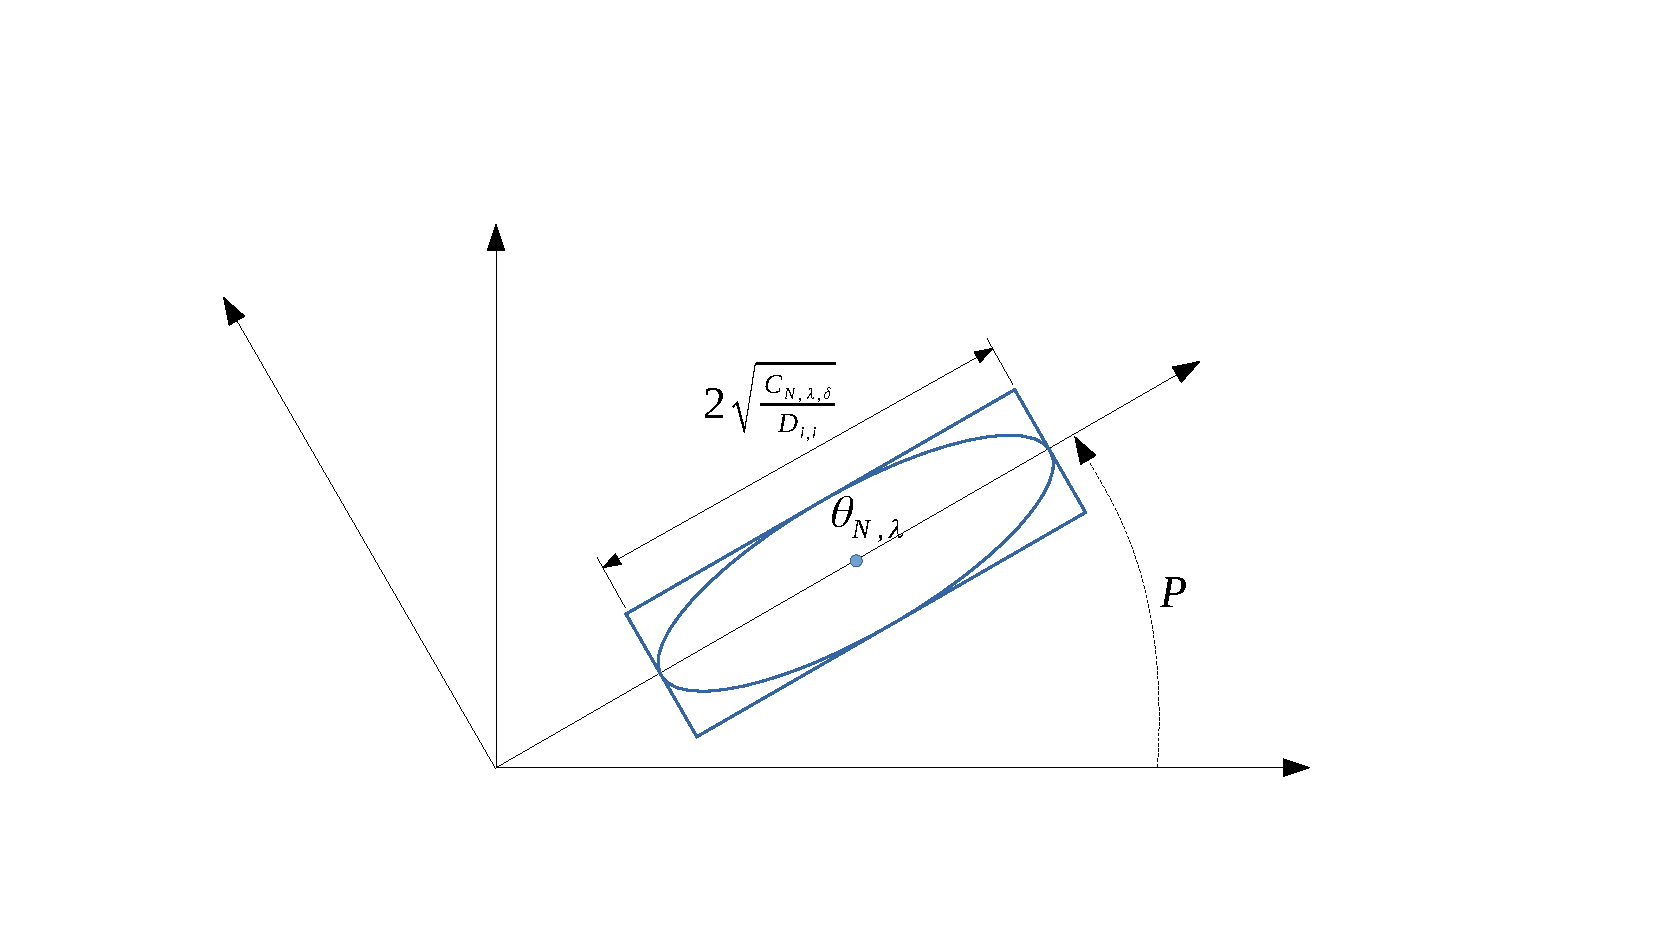
\includegraphics[trim={3.8cm, 2cm, 5cm, 3.8cm}, clip, width=0.7\linewidth]{img/ellipsoid_to_polytope}
		\caption{From the confidence ellipsoid $\cC_\delta$ to its enclosing polytope $\cP_\delta$}
		\label{fig:ellipsoid_to_polytope}
	\end{figure}
	
%		
%	\section{Experimental setting}
%	\label{sec:experimental-setting}
%	
%	In both experiments, we used $\gamma=0.9$,  $\delta=0.9$ and a planning budget $K=100$. The perturbations were sampled uniformly in $[-0.1, 0.1]^r$ while the measurements are Gaussian with covariance $\Sigma_r = 0.1 I_s$. 
%	
%	\subsection{Autonomous Driving}
%	
%	In the following, we describe the structure of the dynamical system $f$ representing the couplings and interactions between several vehicles.
%	
%	\paragraph{Kinematics}
%	
%	The kinematics of any vehicle $i\in[V]$ are represented by the Kinematic Bicycle Model:
%	\begin{align}
%	\dot{x}_i &= v_i\cos(\psi_i), \nonumber\\
%	\dot{y}_i &= v_i\sin(\psi_i), \nonumber\\
%	\dot{v}_i &= a_i, \nonumber\\
%	\dot{\psi}_i &= \frac{v_i}{l}tan(\beta_i), \nonumber
%	\end{align}
%	where $(x_i, y_i)$ is the vehicle position, $v_i$ is its forward velocity and $\psi_i$ is its heading, $l$ is the vehicle half-length, $a_i$ is the acceleration command and $\beta_i$ is the slip angle at the centre of gravity, used as a steering command.
%	
%	\paragraph{Longitudinal control}
%	Longitudinal behaviour is modelled by a linear controller using three features: a desired velocity, a braking term to drive slower than the front vehicle, and a braking term to respect a safe distance to the front vehicle.
%	
%	Denoting $f_i$ the index of the front vehicle preceding vehicle $i$, the acceleration command can be presented as follows:
%	\begin{equation*}
%	a_i = \begin{bmatrix}
%	\theta_{i,1} & \theta_{i,2} & \theta_{i,3}
%	\end{bmatrix} \begin{bmatrix}
%	v_0 - v_i \\
%	-(v_{f_i}-v_i)^- \\
%	-(x_{f_i} - x_i - (d_0 + v_iT))^- \\
%	\end{bmatrix},
%	\label{eq:theta_a}
%	\end{equation*}
%	where $v_0, d_0$ and $T$ respectively denote the speed limit, jam distance and time gap given by traffic rules.
%	
%	\paragraph{Lateral control}
%	
%	The lane $L_i$ with the lateral position $y_{L_i}$ and heading $\psi_{L_i}$ is tracked by a cascade controller of lateral position and heading $\beta_i$, which is selected in a way the closed-loop dynamics take the form
%	
%	\begin{align}
%	\label{eq:heading-command}
%	\dot{\psi}_i &= \theta_{i,5}\left(\psi_{L_i}+\sin^{-1}\left(\frac{\tilde{v}_{i,y}}{v_i}\right)-\psi_i\right),\\
%	\tilde{v}_{i,y} &= \theta_{i,4} (y_{L_i}-y_i). \nonumber
%	\end{align}
%	We assume that the drivers choose their steering command $\beta_i$ such that \eqref{eq:heading-command} is always achieved: $\beta_i = \tan^{-1}(\frac{l}{v_i}\dot{\psi}_i)$.
%	
%	\paragraph{LPV formulation}
%	
%	The system presented so far is non-linear and must be cast into the LPV form. We approximate the non-linearities induced by the trigonometric operators through equilibrium linearisation around $y_i=y_{L_i}$ and $\psi_i=\psi_{L_i}$.
%	
%	This yields the following longitudinal dynamics:
%	\begin{align*}
%	\dot{x}_i &= v_i,\\
%	\dot v_i &= \theta_{i,1} (v_0 - v_i) + \theta_{i,2} (v_{f_i} - v_i) + \theta_{i,3}(x_{f_i} - x_i - d_0 - v_i T),
%	\end{align*}
%	where $\theta_{i,2}$ and $\theta_{i,3}$ are set to $0$ whenever the corresponding features are not active.
%	
%	It can be rewritten in the form $$\dot{X} = A(\theta)(X-X_c) + \omega.$$ For example, in the case of two vehicles only:
%	\begin{equation*}
%	X = \begin{bmatrix}
%	x_i \\
%	x_{f_i} \\
%	v_i \\
%	v_{f_i} \\
%	\end{bmatrix}
%	,\quad
%	X_c = \begin{bmatrix}
%	-d_0-v_0 T \\
%	0 \\
%	v_0\\
%	v_0 \\
%	\end{bmatrix}
%	,\quad
%	\omega = \begin{bmatrix}
%	v_0 \\
%	v_0 \\
%	0\\
%	0\\
%	\end{bmatrix}
%	\end{equation*}
%	
%	\begin{equation*}
%	A(\theta)
%	=
%	\begin{blockarray}{ccccc}
%	& i & f_i & i & f_i \\
%	\begin{block}{c[cccc]}
%	i & 0 & 0 & 1 & 0 \\
%	f_i & 0 & 0 & 0 & 1 \\
%	i & -\theta_{i,3} & \theta_{i,3} & -\theta_{i,1}-\theta_{i,2}-\theta_{i,3} & \theta_{i,2} \\
%	f_i & 0 & 0 & 0 & -\theta_{f_i,1} \\
%	\end{block}
%	\end{blockarray}
%	\end{equation*}
%	
%	The lateral dynamics are in a similar form:
%	\begin{equation*}
%	\begin{bmatrix}
%	\dot{y}_i \\
%	\dot{\psi}_i \\
%	\end{bmatrix}
%	=
%	\begin{bmatrix}
%	0 & v_i \\
%	-\frac{\theta_{i,4} \theta_{i,5}}{v_i} & -\theta_{i,5}
%	\end{bmatrix}
%	\begin{bmatrix}
%	y_i - y_{L_i} \\
%	\psi_i - \psi_{L_i}
%	\end{bmatrix}
%	+
%	\begin{bmatrix}
%	v_i\psi_{L_i} \\
%	0
%	\end{bmatrix}
%	\end{equation*}
%	Here, the dependency in $v_i$ is seen as an uncertain parametric dependency, \emph{i.e.} $\theta_{i,6}=v_i$, with constant bounds assumed for $v_i$ using an overset of the longitudinal interval predictor.
%	
%	
%	\paragraph{Change of coordinates}
%	In both cases, the obtained polytope centre $A_0$ is non-Metzler.
%	We use the similarity transformation of coordinates of \citet{Efimov2013}. Precisely, we choose $\Theta$ such that for any $\theta\in\Theta$, $A(\theta)$ is always diagonalisable with real eigenvalues, and perform an eigendecomposition to compute its change of basis matrix $Z$. The transformed system $X'=Z^{-1}(X-X_c)$ verifies \eqref{eq:confidence} with $A_0$ Metlzer as required to apply the interval predictor of \autoref{prop:predictor}. Finally, the obtained predictor is transformed back to the original coordinates $Z$ by using the following lemma:
%	\begin{lemma}[Interval arithmetic of \citealt{Efimov2012}]
%		\label{lem:interval} Let $x\in\mathbb{R}^{n}$ be a vector variable, $\underline{x}\le x\le\overline{x}$ for some $\underline{x},\overline{x}\in\mathbb{R}^{n}$. 
%		
%		\begin{enumerate}
%			\item If $A\in\Real^{m\times n}$ is a constant matrix, then
%			\begin{equation}
%			A^{+}\underline{x}-A^{-}\overline{x}\le Ax\le A^{+}\overline{x}-A^{-}\underline{x}.\label{eq:Interval1}
%			\end{equation}
%			\item If $A\in\Real^{m\times n}$ is a matrix variable and \textup{$\underline{A}\le A\le\overline{A}$} for some $\underline{A},\overline{A}\in\Real^{m\times n}$, then
%			\begin{gather}
%			\underline{A}^{+}\underline{x}^{+}-\overline{A}^{+}\underline{x}^{-}-\underline{A}^{-}\overline{x}^{+}+\overline{A}^{-}\overline{x}^{-}\leq Ax\label{eq:Interval2}\\
%			\leq\overline{A}^{+}\overline{x}^{+}-\underline{A}^{+}\overline{x}^{-}-\overline{A}^{-}\underline{x}^{+}+\underline{A}^{-}\underline{x}^{-}.\nonumber 
%			\end{gather}
%		\end{enumerate}
%	\end{lemma}
	
%	\paragraph{Actions}
%	
%	The action space $\cA$ is constituted of five actions: faster, slower, lane change to the right, lane change to the left, and no-op. They are implemented by a lateral linear controller that track a reference lateral position $y_L$, affected by the lane change actions, and a lateral longitudinal linear controller that tracks the desired velocity $v_0$, affected by the faster and slower actions.
%	
%	\paragraph{Reward}
%	
%	The reward function $R$ is the following:
%	\[
%	R(x) = 
%	\begin{cases}
%	1 & \text{if the ego-vehicle is at full velocity;}\\
%	0 & \text{if the ego-vehicle has collided with another vehicle;}\\
%	0.5 & \text{else.}
%	\end{cases}\]
	
\end{subappendices}
